\chapter{Solution}


\section{Overview} 

The goal of the thesis is to develop a software application, blockchain-based, for a Fashion company. The fashion 
company wants a blockchain solution to handle the internal processes with a tracking mechanism of the clothes over 
the supply chain. There are many actors involved in the system, therefore, the software has to implement a membership 
mechanism to handle access over the network. Moreover, for the sustainability issue, the company wants to introduce an 
asset token exchanged with the clothes, which represents the CO\textsubscript{2} emission saved. Therefore the token 
must be run over a public blockchain in order to be detached by own use.   
\bigskip

Below there is the thesis work overview. I listed the technologies used for the solution, the work produced and the main
processes of the thesis. 

\subsection{Actors}

The main \textbf{actors} involved in the system are three:

\begin{outline}
    \1 \textbf{User}: It is the \textit{end-user}. It uses the web-app to \textit{send old clothes} and \textit{purchase items} from Reclothes store.
    The User is the actor that starts the entire process flow, sending the clothes. This action is mandatory for the whole process. 
    \1 \textbf{Reclothes Admin}: It is the \textit{system admin}, it performs the actions in order to handle the system.
    The Reclothes Admin handles both parts, User Side and Producer Side. About User Side, it performs a set of actions
    in order to \textit{handle} in the best way \textit{the clothes arrived and the tokens provided}. On the other hand, Producer Side, the Admin
    cares about to \textit{handling the recycling and upcycling process}, providing the old materials to the Producer
    and spend, when the platform needs, the token received to order recycled clothes.  
    \1 \textbf{Producer}: It is part of the upcycling process. It receives the materials to \textit{perform the recycling process}.
    In the test case, I consider just one Producer, that receives the entire old materials to be recycled.
    However, the system is developed in order to allow a set of Producers registered. It allows the Reclothes Admin,
    during the Send Old Clothes process, to choose the Producer toward which ship the material. 
\end{outline}

\subsection{Work Produced}

\textbf{Figure \ref{fig:schema}} shows the overview and the main flow of the overall application.
The overall system and the thesis work produced to create the application is composed of the following parts:
\begin{outline}
    \1 \textbf{Networks}: They are the networks over which the blockchains run. The project involves two kinds of networks:
    \2 \textbf{Hyperledger Fabric Network}: the main network. I choose Hyperledger Fabric because it has a highly modular 
    architecture and it implements a well-defined membership mechanism. Fabric is a solid network and provides at the 
    developers a lot of instruments that simplify the implementation process.  
    \2 \textbf{Ethereum Network}: the side network used for token exchanged for own use. The Ethereum is a strong 
    reality and widely used to develop solutions applied to the public blockchain. It provides huge tools and instruments 
    that allow the developers to develop contracts easily. In this thesis work is used the Ropsten testnet.    
    \1 \textbf{Shell Scripts}: to set up everything in the best way, it is produced a set of 
    shell scripts that run network or shut it down, install chaincode, and run part of the system mandatory 
    for the application use. 
    \1 \textbf{Smart Contracts}: The smart contracts perform project use case actions. 
    There are three smart contracts. Each contract performs one specific flow and includes just
    a set of the overall actors involved in the system.  
    \1 \textbf{Dapp}: It is the web application, it allows the actors to interact with the system. It is a 
    decentralized application that communicates with the blockchain networks. Once the user is logged in, 
    with related rights, he can perform smart contracts invocation using the web-app.
\end{outline}

\subsection{Application Flow}

Each actor accesses to the system with different permission and privileges. Once logged in, 
the user can access to several features and he can performs a set of actions over the system. 
For a better understanding, we are going to split the overview flow shown in \textbf{Figure \ref{fig:schema}} 
into 2 sub-flow starting from Reclothes actor, considered as the \textit{System Admin}, 
the \textbf{User side} on the left side and the \textbf{Producer side} on the right side. 

\bigskip

Each side has a set of main actions that are going to modify the world state of the blockchains.
Based on that principle, the smart contract invocations are going to produce transactions that modify the 
ledgers in an immutable way, adding a new block to the chains. The main processes are the following: 

\begin{outline}[enumerate]
	\1 \textbf{User Side}
    \2 User sends Box with old clothes and receive Fabric points and ERC20 Token.
    \2 User purchases items inside dapp store using Fabric points and ERC20 Token.
    \1 \textbf{Producer Side}
    \2 Reclothes send clothes box with old materials and receive Regeneration Credits.
    \2 Reclothes spend the Regeneration Credits to purchase upcycled clothes by Producer.
\end{outline}

these processes are described in detail in the \ref{use-cases} section, which analyzes 
deeper the transactions process. 

\begin{figure}[h!]
	\centering
	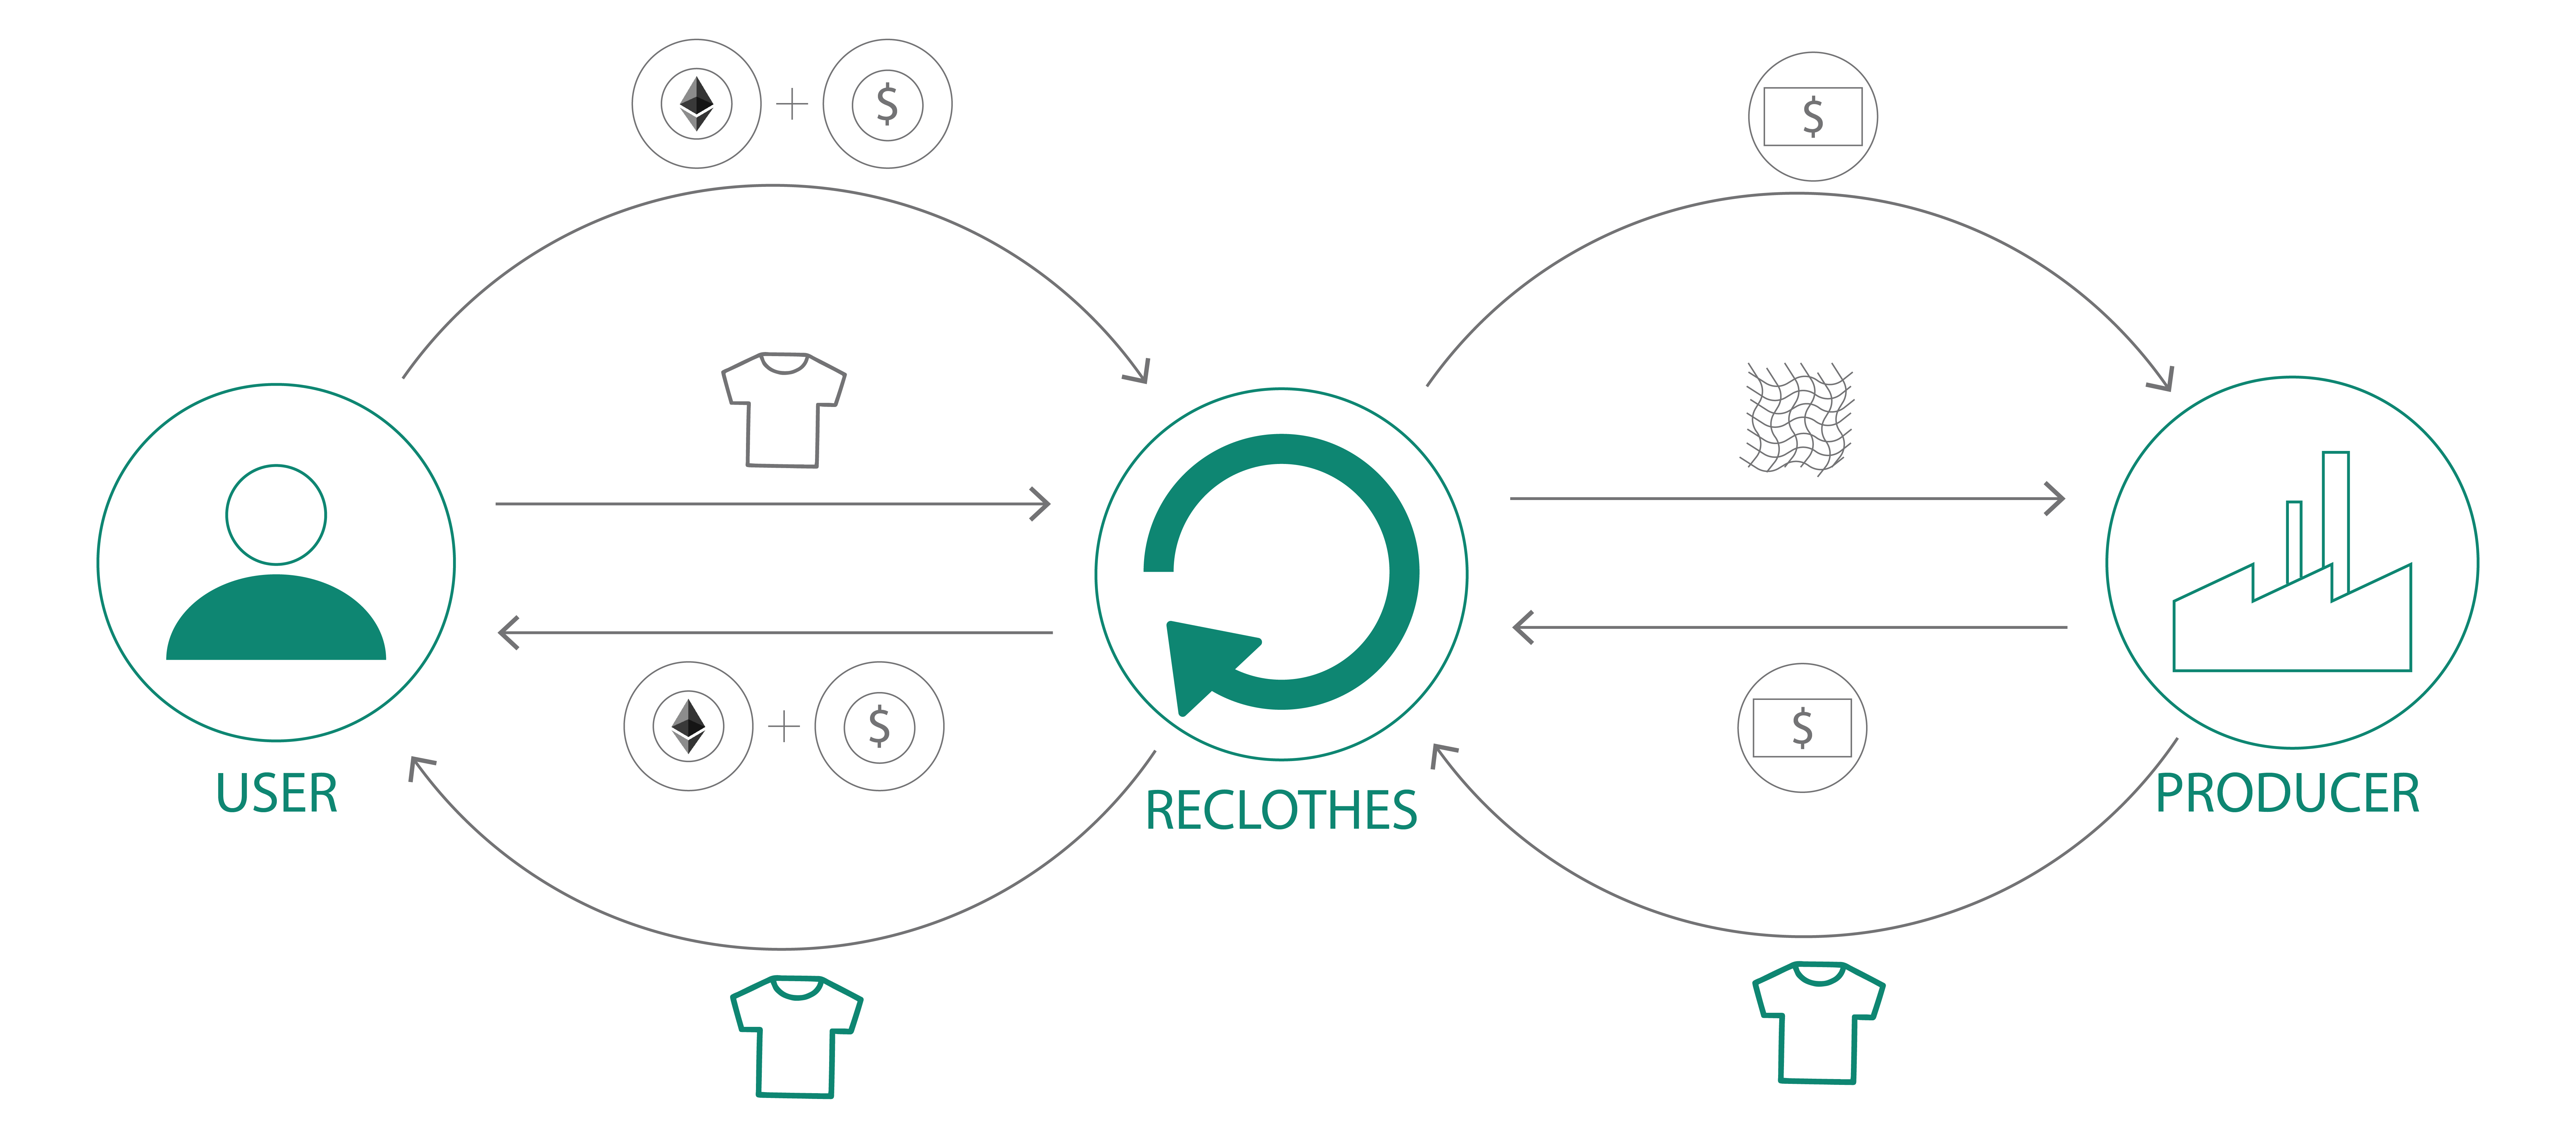
\includegraphics[totalheight=6cm]{img/use-case-schema.png}
	\caption{UseCase Overview}
	\label{fig:schema}
\end{figure}

\subsection{Token exchanged}

There are two \textbf{Token} categories exchanged over the networks. 
\bigskip

Hyperledger Fabric side is exchanges two kinds of tokens, both are point-based, integrated with the smart 
contracts that handle User and Producer side both. The User points are handled Reclothes side, which means that 
the Reclothes Admin decides the amount to be sent to the User. 
In order to handle the amount of the transaction and establish a standard behavior, it needs a reference table that 
sets a fixed amount for each clothes received. The producer side points, \textit{Regeneration Credits}, are 
handled by the Producer side, is the Producer that receives the old materials, and then choose the amount to 
be sent. As the User points, it needs a table to fix rules for the corresponding amounts for the received 
materials evaluation. 
\bigskip

On the other side, there is the ERC20 token that runs over the Ethereum network. ERC20 is a standard 
protocol that allows everyone to implement its token following fixed rules. That standard includes a 
set of fixed operations: \texttt{totalSupply, balanceOf, transfer, transferFrom, approve 
and allowance}. 

\bigskip
To clarify the tokens exchanged over the thesis work and their behavior, here is a list below:

\begin{outline}[enumerate]
	\1 \textbf{Over Fabric Network}
    \2 \textbf{User Token}: It is a token, points-based, used to handle part of the payment system related to clothes
    shipping from User to Reclothes and vice-versa.
    \2 \textbf{Regeneration Credits}: It is a token, points-based, used to handle the credit system related to clothes
    shipping from Reclothes to Producers and vice-versa.

    \1 \textbf{Over Ethereum Network}
    \2 \textbf{CO2 Token}: It is and ERC20 Token run over public network in charge to handle part of the payments related 
    to clothes shipping from User to Reclothes and vice-versa.
\end{outline}


%CROSSCHAIN
\clearpage
\section{CrossChain interaction}

\subsection{Why a cross-chain solution is needed}

One of the goals of the thesis work is to implement a good integration between the two blockchain networks 
involved in the system. The need for a cross-chain solution applied to own cases is to keep the 
\textbf{\texttt{CO\textsubscript{2} Token}} exchanged public, so that, for the future use, it can be 
reused in other environments and applications. In that way, the token is not strictly correlated to own 
personal use, but it could become a standard token to be exchanged over Ethereum, and corresponding to an 
asset related to CO\textsubscript{2} emissions. The behavior of that token is better analyzed in \ref{erc20} 
section.
\bigskip

The main requirement to obtain a good integration is to perform cross-chain process without compromise the 
security issue both sides, Fabric and Ethereum. Therefore we need to care about the technologies behaviors 
and what's the technical basis upon which blockchains works. 
\bigskip

Before introducing the chosen solution, it is important to have a look at the technologies used for 
thesis development. 

\subsection{Technologies Used}

Below there are all the main technologies used, involved in the application, and in the cross-chain process.
\textbf{Figure \ref{fig:architectural-flow}} shows how these technologies and tools are used and 
interact with each other. 

\begin{outline}
    \1 \textbf{Hyperledger Fabric}: Hyperledger Fabric is a modular blockchain framework that acts as a foundation for 
    developing blockchain-based products, solutions, and applications using plug-and-play components that are aimed for 
    use within private enterprises. 
    \1 \textbf{Ethereum}: Ethereum is an open-source, blockchain-based, decentralized software platform. It enables 
    to build and run smart contracts and distributed applications (DApps).
    \1 \textbf{Metamask}: It is used as Ethereum wallet to perform and sign the transactions started by dapp.
    Exploiting Metamask API, a high level of security is granted to perform transactions over the Ethereum network. 
    It is integrated into the thesis work Application side; for the right usage of the entire application is
    mandatory that the User is logged in Metamask over the wallet specified during the registration phase.  
    \1 \textbf{Web3}: It is the software library used to interact with smart contracts.
    The Web3.js API fulfills the developers' needs for the integration between website/client and Ethereum blockchain.
    It is a collection of libraries that allows developers to perform actions like sending Ether from one account to another, read 
    and write data from smart contracts, create smart contracts, and much more. 
    \1 \textbf{Fab3 Proxy}: It maps the Web3 API with the Fabric SDK in order to interact with
    Fabric network. It performs a mapping between the Fabric Identity (X.509) with an Ethereum address, generated on the fly,
    used to perform dapp calls. In other words, it works like a bridge between Ethereum technologies and tools, used 
    for dapp development, and Fabric chaincode, that run over the Fabric peers and use the GO SDK to allow 
    the chaincode invocation.  
    \1 \textbf{Fabric Chaincode EVM}: It is the Ethereum Virtual Machine chaincode that allows running Solidity smart contracts
    over the Fabric network. It is a core part of the entire thesis work. Thanks to EVM chaincode it is
    possible to run solidity bytecode over Fabric peers.
    \1 \textbf{Remix}: It is an online editor that allows developing well-structured Solidity smart contracts. 
    Thanks to the plugins, that could be installed over the editor, it is possible to compile the written 
    smart contracts code. Once the compiling process succeeds, it produces the corresponding smart contract's 
    bytecode and the smart contract's ABI. Both bytecode and ABI are used to define smart contract behaviors. These parameters are passed as an argument during the deployment process. 
    \1 \textbf{Expressjs}: It is a web framework used to develop web-app and smart contract API.
    It's a light, easy, and fast framework that integrates several methods useful for HTTP and middleware API development. 
    \1 \textbf{Infura}: It allows running an Ethereum node, to set an endpoint used to interact with the 
    contract. It allows in an easy way to set up a public endpoint for the deployed contract address. 
    It provides personal API and key for the endpoint access. Moreover, it provides a well defined and 
    detailed dashboard to analyze all the smart contract invocations, providing deeper analyses for the 
    called method too.  
    \1 \textbf{Docker}: The Fabric network components run inside Docker containers. It is mandatory
    for Fabric network blockchains, each peer(node) of the network run inside a specific and 
    dedicated container. It allows being monitored and analyzed independently. 
\end{outline}
\bigskip

Thanks to the introduction of the EVM chaincode developed by the IBM technical ambassadors,
it is possible to run Solidity bytecode over the Fabric network. It allows the possibility to joint 
Ethereum technologies over Hyperledger Fabric Network.
That innovation doesn't improve only the integration network side but developing side too. With the 
\texttt{fabric-chaincode-evm} a new communication way from dapp/client side is open to the network side.
For example, that integration allows to use Web3.js library to invoke smart contracts running over Fabric. 
Moreover, most of the improvements done in the Ethereum environment can be used to interact with the 
Hyperledger Fabric world. It means languages, API, libraries, and tools that are finding a huge application 
in the Ethereum world, so far. 
\bigskip

The cross-chain solution chosen involves the Application Layer. The core idea of the solution is to map, at 
the Application level, the Ethereum wallet with Hyperledger Fabric identity. Once there is a one-to-one 
association, is used the eth wallet for transactions over Ethereum network and the related Fabric 
identity over Fabric network. Exploiting Web3.js API we invoke Ethereum or Fabric smart contracts, by using 
this solution all the invocation processes are forward, to the corresponding network, starting from Dapp 
API. 
\bigskip

The authentication mechanism doesn't change and the security continues to be ensured, Fabric side, using 
certificate x.509. Once the user is authenticated and recognized by the x.509 certificate, Fabric network 
logged the user into the platform and give him the access to the data information and all the related 
privileges based on the actor role.
\bigskip

On the other hand, Ethereum side, the user Ethereum public address is specified
during the registration phase and saved over Fabric chaincode to the corresponding User data structure.
When the user is involved inside transaction processes, all the transactions refer to the public Ethereum
address reported during the registration phase. 
\bigskip

Therefore when there is an incoming transaction the tokens will be sent to the public address reported in User Data info. 
When an outgoing transaction occurs, the security is granted thanks to the Metamask integration in the 
transaction process. The transaction's sign, that allows performing operation, is performed by Metamask side, 
in that way only the real owner of the Ethereum account could sign and approve the transaction. The private 
key is stored over Metamask wallet and just the real owner, that is logged in to the account, can perform 
the sign of the transaction. 
\bigskip  

Furthermore, the dapp client uses Fab3 Proxy to map the identity from Ethereum address to Fabric
identity x.509 certificate and forward request to Fabric network. That process is independent by the Ethereum address
specified during the registration phase and does not interact with that. Fab3 allows to use \texttt{fabric-chaincode-evm} 
and run solidity code over Fabric network, It performs a mapping process among the received requests dapp side.
Fab3 receives the Web3 request and map it using the GO SDK to forward, in the right way, all the request
to the Fabric peers. 
\bigskip

Moreover, the Dapp client talks with Ethereum public blockchain network, using the network endpoint API supplied by Infura. 
For some kind of actions performed over the platform, part of the request is forward over Ethereum network. 

\begin{figure}[h]
	\centering
	\includegraphics[totalheight=14cm]{img/architectural_flow.png}
	\caption{Architectural Flow}
    \label{fig:architectural-flow}
\end{figure}
\bigskip

\textbf{Figure \ref{fig:keys}} shows where the private keys are stored. The Hyperledger wallet could be stored in many 
ways, into a FileSystem, in memory, using a HSM or a Database\cite{fabric-wallet}. For the thesis work, I consider
the device filesystem storage, containing the Hyperledger wallet with the certificate and both private and public keys.
Always on the device used, it is stored the private key of the Ethereum wallet, in fact, Metamask store on the device
the private key of the associated Ethereum account\cite{metamask}.  
 
\begin{figure}[h]
	\centering
	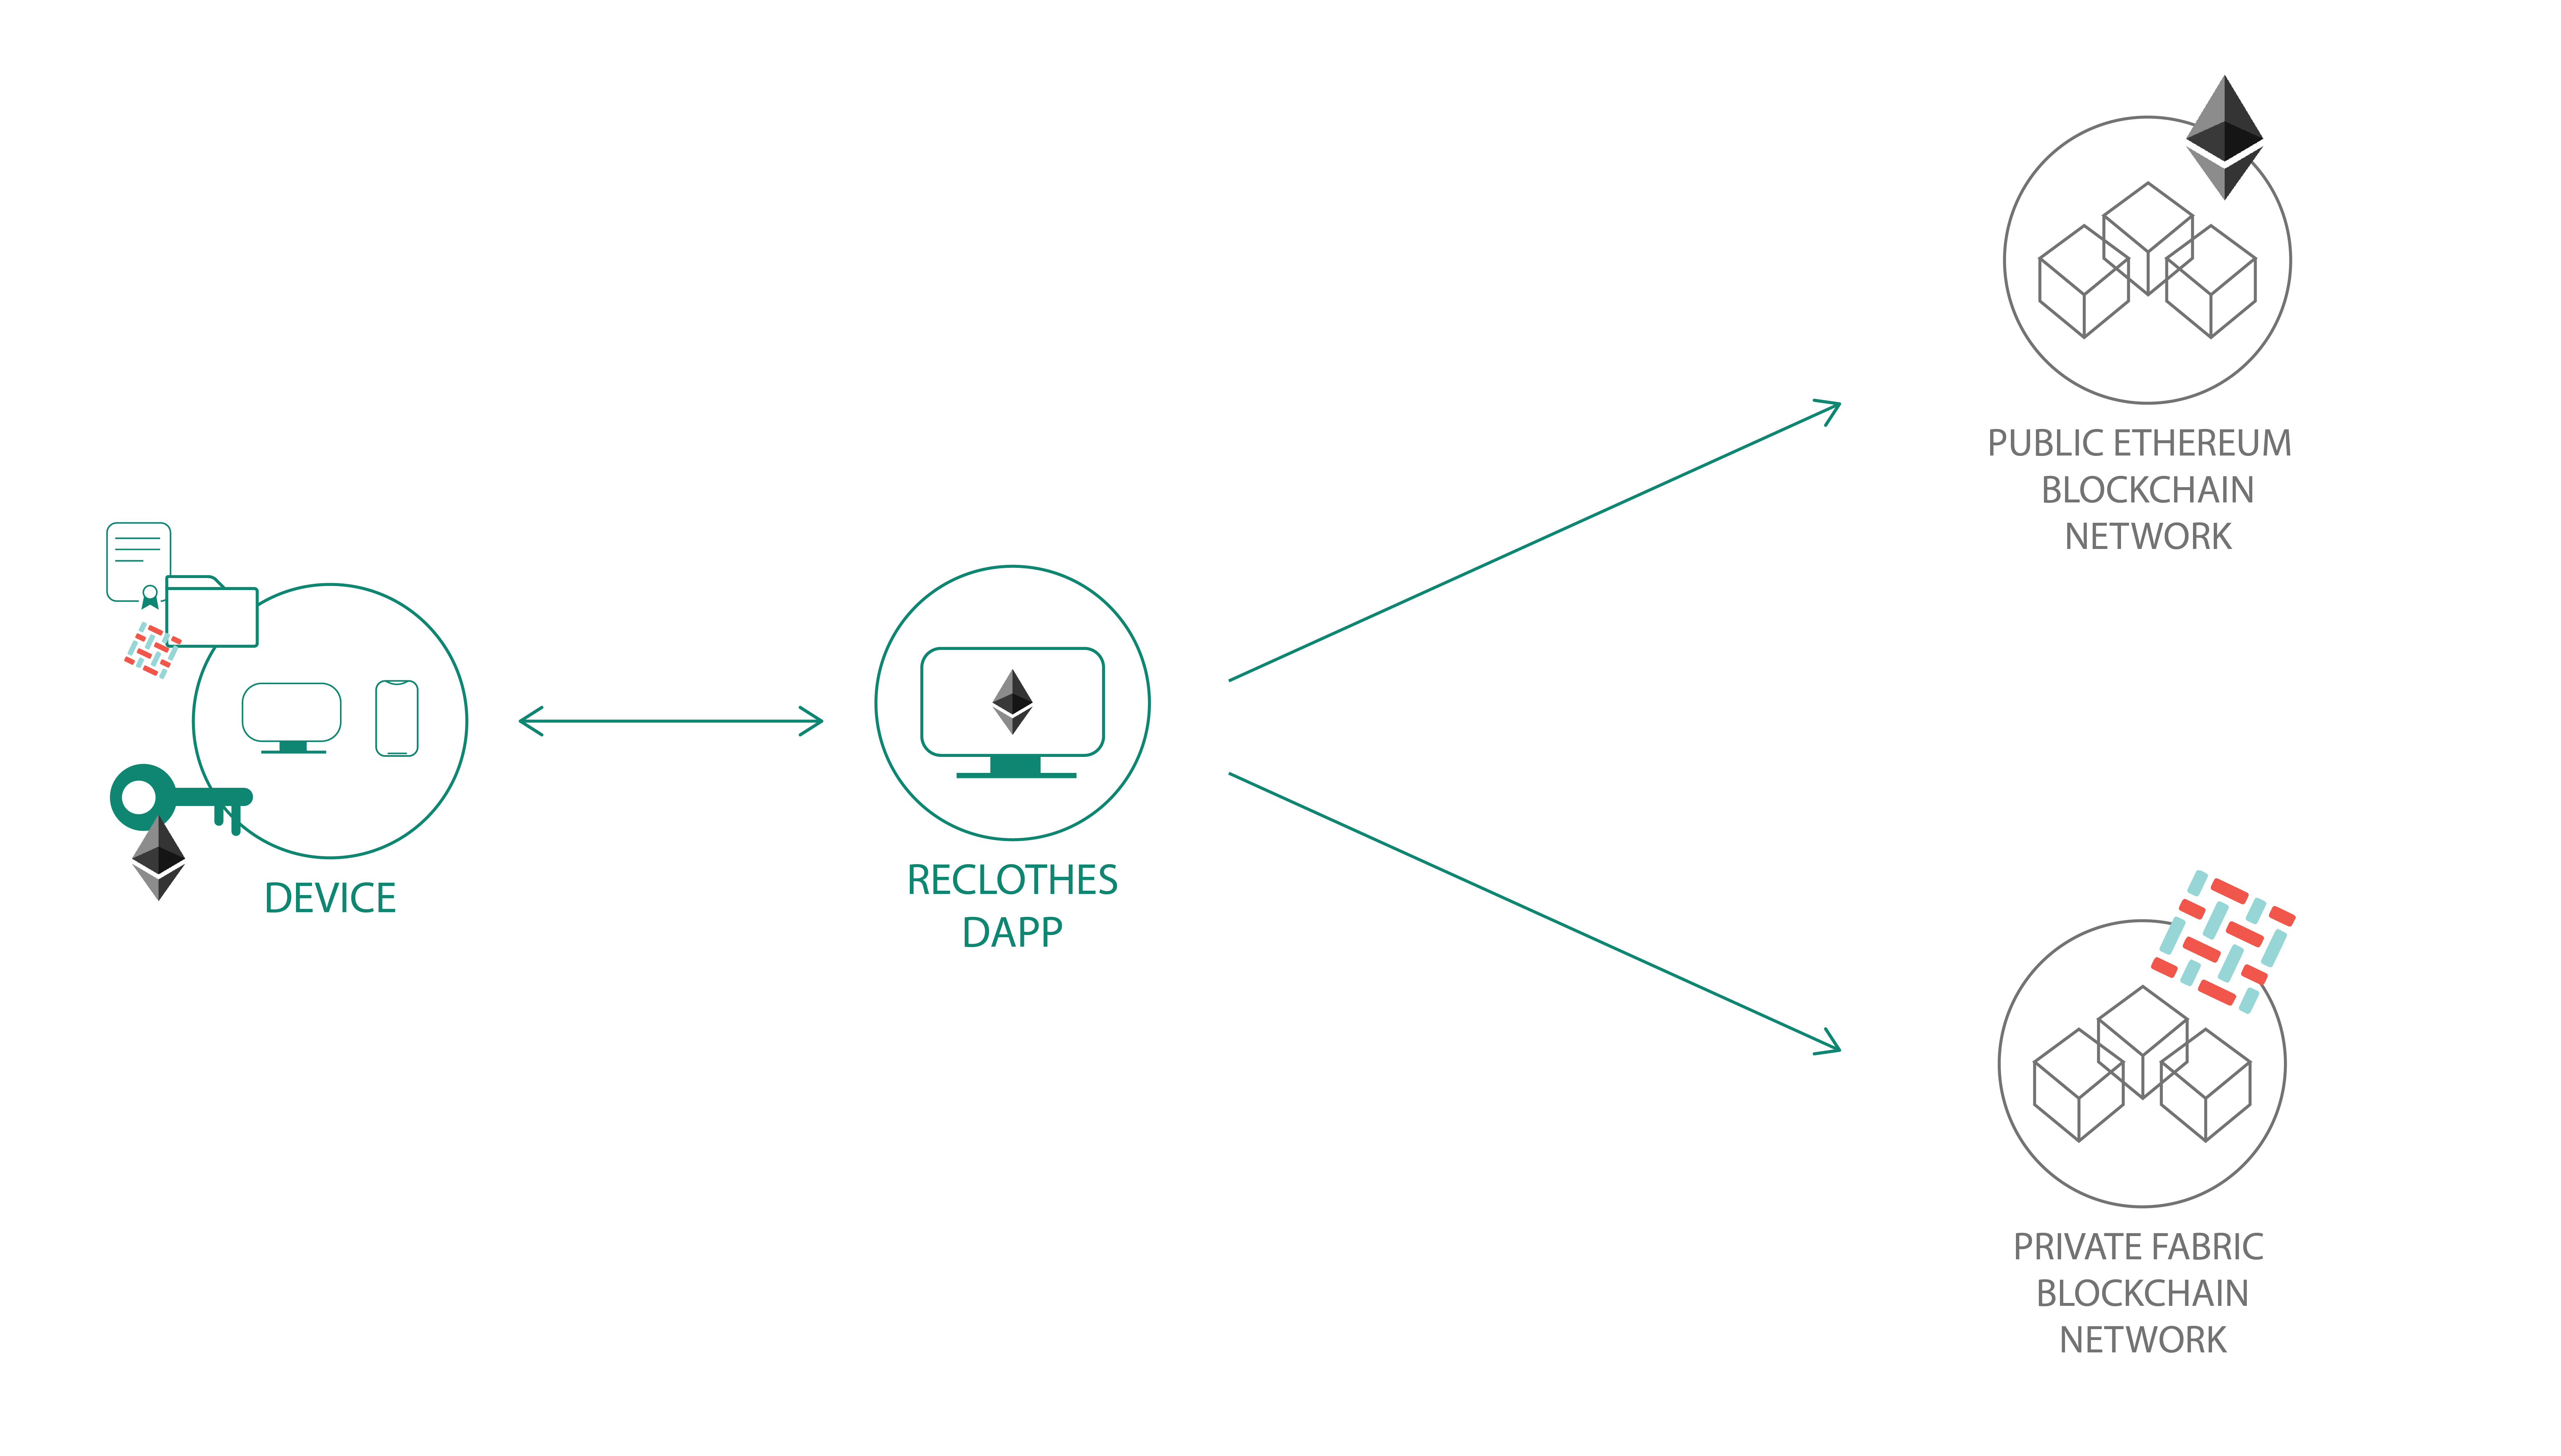
\includegraphics[totalheight=8cm]{img/keys.png}
	\caption{Where keys are stored}
    \label{fig:keys}
\end{figure}

%USE CASES
\clearpage
\section{Use Cases}
\label{use-cases}

As explained in the previous sections, for a better outline, the use cases are splint inside the 
\textbf{User Side} and the \textbf{Producer Side}. The main actor of the system is still Reclothes Admin, 
that is linked to both side and interacts with all the other actors in order to supply the management 
supports that allow the entire system works.

\subsection{UseCase 1 - User Side}

As shown in \textbf{Figure \ref{fig:usecase1}} both actors User and Reclothes Admin, once logged in, have access to a set
of features. The use case diagram shows all the actions that both users can perform over the networks and
the flows that each action follows. The features are split over the two networks, the Fabric one and the 
Ethereum one. All the flows start from one of the two actors involved and in the end it merges to one 
of the two blockchain networks. Each actor has a dedicated Ethereum wallet used for Ethereum token
transactions. 
\bigskip

Below is listed and analyzed all the actions that users could perform over the system:
\begin{outline}
    \1 \textbf{Actions in common}
    \2 \textbf{Registration}: The registration phase involves the actor that fills a form with all the 
    mandatory data. To proceed to a successful registration process it is mandatory that the actor
    owns the appropriate x.509 certificate, released by the Certification Authority related to the Role
    in which the user tries to sign up. For example, User has a specific Certification Authority that is
    different from Reclothes CA. 
    \2 \textbf{Sign In}: The sign-in is automatic. Once the Fabric network recognizes the certificate, 
    it proceeds to log the actor in, with the related rights. Once the user is logged in, the chaincode 
    is invoked and going to read the Ethereum address( generated by Fab3 ) used for the registration phase 
    and provide access to the methods. In other words, Fabric certificate provides access to the network 
    (peers, channels, and ledger), instead, the Ethereum address(Fab3 side) is used to provide access to 
    the smart contract. 
    
    \1 \textbf{User Operations}
    \2 \textbf{Read Operations}
    \3 \textbf{View own transactions}: once logged in, the User can view all the own transactions 
    processed by the network, with a flag that shows transaction status. The transactions include token 
    exchanged over the network and box requests sent to Reclothes. It gave the possibility to monitor and 
    manage each process in which the User is involved. 
    \2 \textbf{Write Operations}
    \3 \textbf{Send Box}: It is the starting point of the overall application flow. In the following 
    subsection, I'm going deeper in order to explain how that process works and what transactions depend 
    on that.
    \3 \textbf{Purchase Items}: It is a write operation, belongs to that start a transaction process. 
    Both networks are involved in that process. Even that is explained deeper in the following subsection.

    \1 \textbf{Reclothes Admin Operations}
    \2 \textbf{Read Operations}
    \3 \textbf{View all transactions}: once is logged in, the Reclothes Admin can view all the transactions 
    processed by the network related to all the users involved, with a flag that shows transaction status. 
    The transactions include a token exchanged over the network. It gave the possibility to monitor and manage 
    each process in which there is a token transactions for analysis aim.
    \3 \textbf{View All Box Requests}: The Admin is allowed to analyze the process of the box shipping.
    The box data structure includes all the relevant data. Moreover, it includes a flag that specifies the status
    of the request, that flag could be \texttt{Pending, Evaluated}. 
    \2 \textbf{Write Operations}
    \3 \textbf{Evaluate Box}: Even this process belongs to write operations because it starts a transaction process 
    that writes the blockchain world state. 

\end{outline}


The main action of the overall system is the send box operation performed by the User towards Reclothes.
It is the starting point of the overall flow. The Internal Flow of the \textit{\bf{Send Box}} macro 
process, and what that process belongs to, is the following one:

\begin{outline}[enumerate]
    \1 User send box with old clothes
    \1 Reclothes Admin receive box, evaluate it
    \1 The web app performs the payments from Reclothes Account to User Account
    \1 Once both transactions succeed, both tokens are accredited and User could spend it
\end{outline}

\subsubsection{Transactions}

In the first use case both the blockchain networks are involved in. The main part of the flow and the most critical one is the 
transaction process. Considering always \textit{Reclothes Admin} the main actor of the system, there are two kinds 
of transactions in which Admin is involved. 
The \texttt{outgoing} transaction, that starting by \texttt{Evaluation} process, it is performed by the Reclothes Admin once 
it receives the clothes box sent by the User. The other one is the \texttt{incoming} transaction, in that case, the 
token is exchanged from the User to Reclothes Admin. The action that starts the incoming transaction process is the 
\texttt{Purchase Item}, performed by the Users over the platform store.
\bigskip

The outgoing and incoming transactions are strictly correlated due to the token flow. As explained in the previous 
section the main and the first one action is the \texttt{Send Box}, which involves the \texttt{Evaluation}.
The Evaluation is the first outgoing transaction process performed over the system. Once the tokens are moved from the 
Reclothes Admin, the User is allowed to use applications and purchase items over it.

\begin{outline}[enumerate]
    \1 \textbf{Figure \ref{fig:evaluation}} shows the \textit{\bf{Evaluation}} process, which works in the following way:
    \2 Reclothes Admin visualizes the next pending request to be evaluated. The Admin visualizes all the related information
    associated to the box request: \texttt{userAddress} it's the Ethereum user address of the sender, 
    \texttt{t-shirt, pants, jacket, other} with the related number of items associated to the request,
    and the status of the request, at this point still \texttt{In Pending}.
    \2 Reclothes Admin evaluates it. For a better evaluation process, it is proposed a solution based on a reference table 
    with a fixed amount for each item, related to the clothes status. Then there is a filtering process. Each item 
    inside the box is filtered based on platform criteria. Then the Admin decides the status of the clothes and its 
    final destination, which may be the platform store or recycling materials. Once the overall clothes are 
    evaluated and are set a total amount value of Fabric points and ERC20 Token is set, the transaction process can start.
    \3 The Fabric points are sent over Fabric network invoking the chaincode function \texttt{sendPoints(address toAddress)}.
    That function accredited the specified amount of Fabric points, updating the User balance. 
    \3 The ERC20 token is sent over the Ethereum network. During the thesis development, I have used the Ropsten testnet 
    to exchange the token. There is a previous step before performing the transaction of the tokens. The Fabric 
    chaincode is invoked to obtain the Ethereum wallet address related to the sender box User. Once that the Fabric 
    chaincode returns the Ethereum account, stored in the smart contract during the User Registration Phase, the 
    application performs the transfer of the ERC20 token from the Reclothes wallet to the User Ethereum wallet
    \2 Once both transactions succeed, both the transaction return to the application and is performed
    an additional check in order to synchronize both transactions. Tokens are accredited and 
    information about balances are updated. From that moment the User can spend the received
    tokens over the platform store, performing purchasing. 

    \1 \textbf{Figure \ref{fig:purchase}} shows the \textit{\bf{Purchase Items}} process, which works in a similar way, but inverting the previous flow:
    \2 The User chooses the items to purchase over the web-app store. The items (t-shirt, pants, jacket, or other) 
    are represented with the related form, which shows all the relevant information. Over the chaincode the smart 
    contract store a dedicated data structure for clothes data information. The related price is expressed through 
    tokens, Fabric token and CO\textsubscript{2} token both. 
    \2 Once the items are chosen, the purchase process starts. The User sends the Fabric tokens over Fabric network 
    and the CO\textsubscript{2} token over the Ethereum network. First of all, a set of controls is executed 
    in order to check both balances and evaluate whether the User could perform the purchase transaction. Once that all 
    the check is passed correctly, both transactions start.
    Each one over the dedicated network. Once the transfer process is performed, the smart contracts return the 
    operation results to the dapp, that communicate the results of the operations through a message .
    \2 If the transfers succeed, both token balances are updated and the User can
    continue to perform actions over the platform.    
\end{outline}

\begin{figure}[h!]
	\centering
	\includegraphics[totalheight=15cm]{img/use_case1.png}
	\caption{UseCase 1}
	\label{fig:usecase1}
\end{figure}

\begin{figure}[h!]
	\centering
	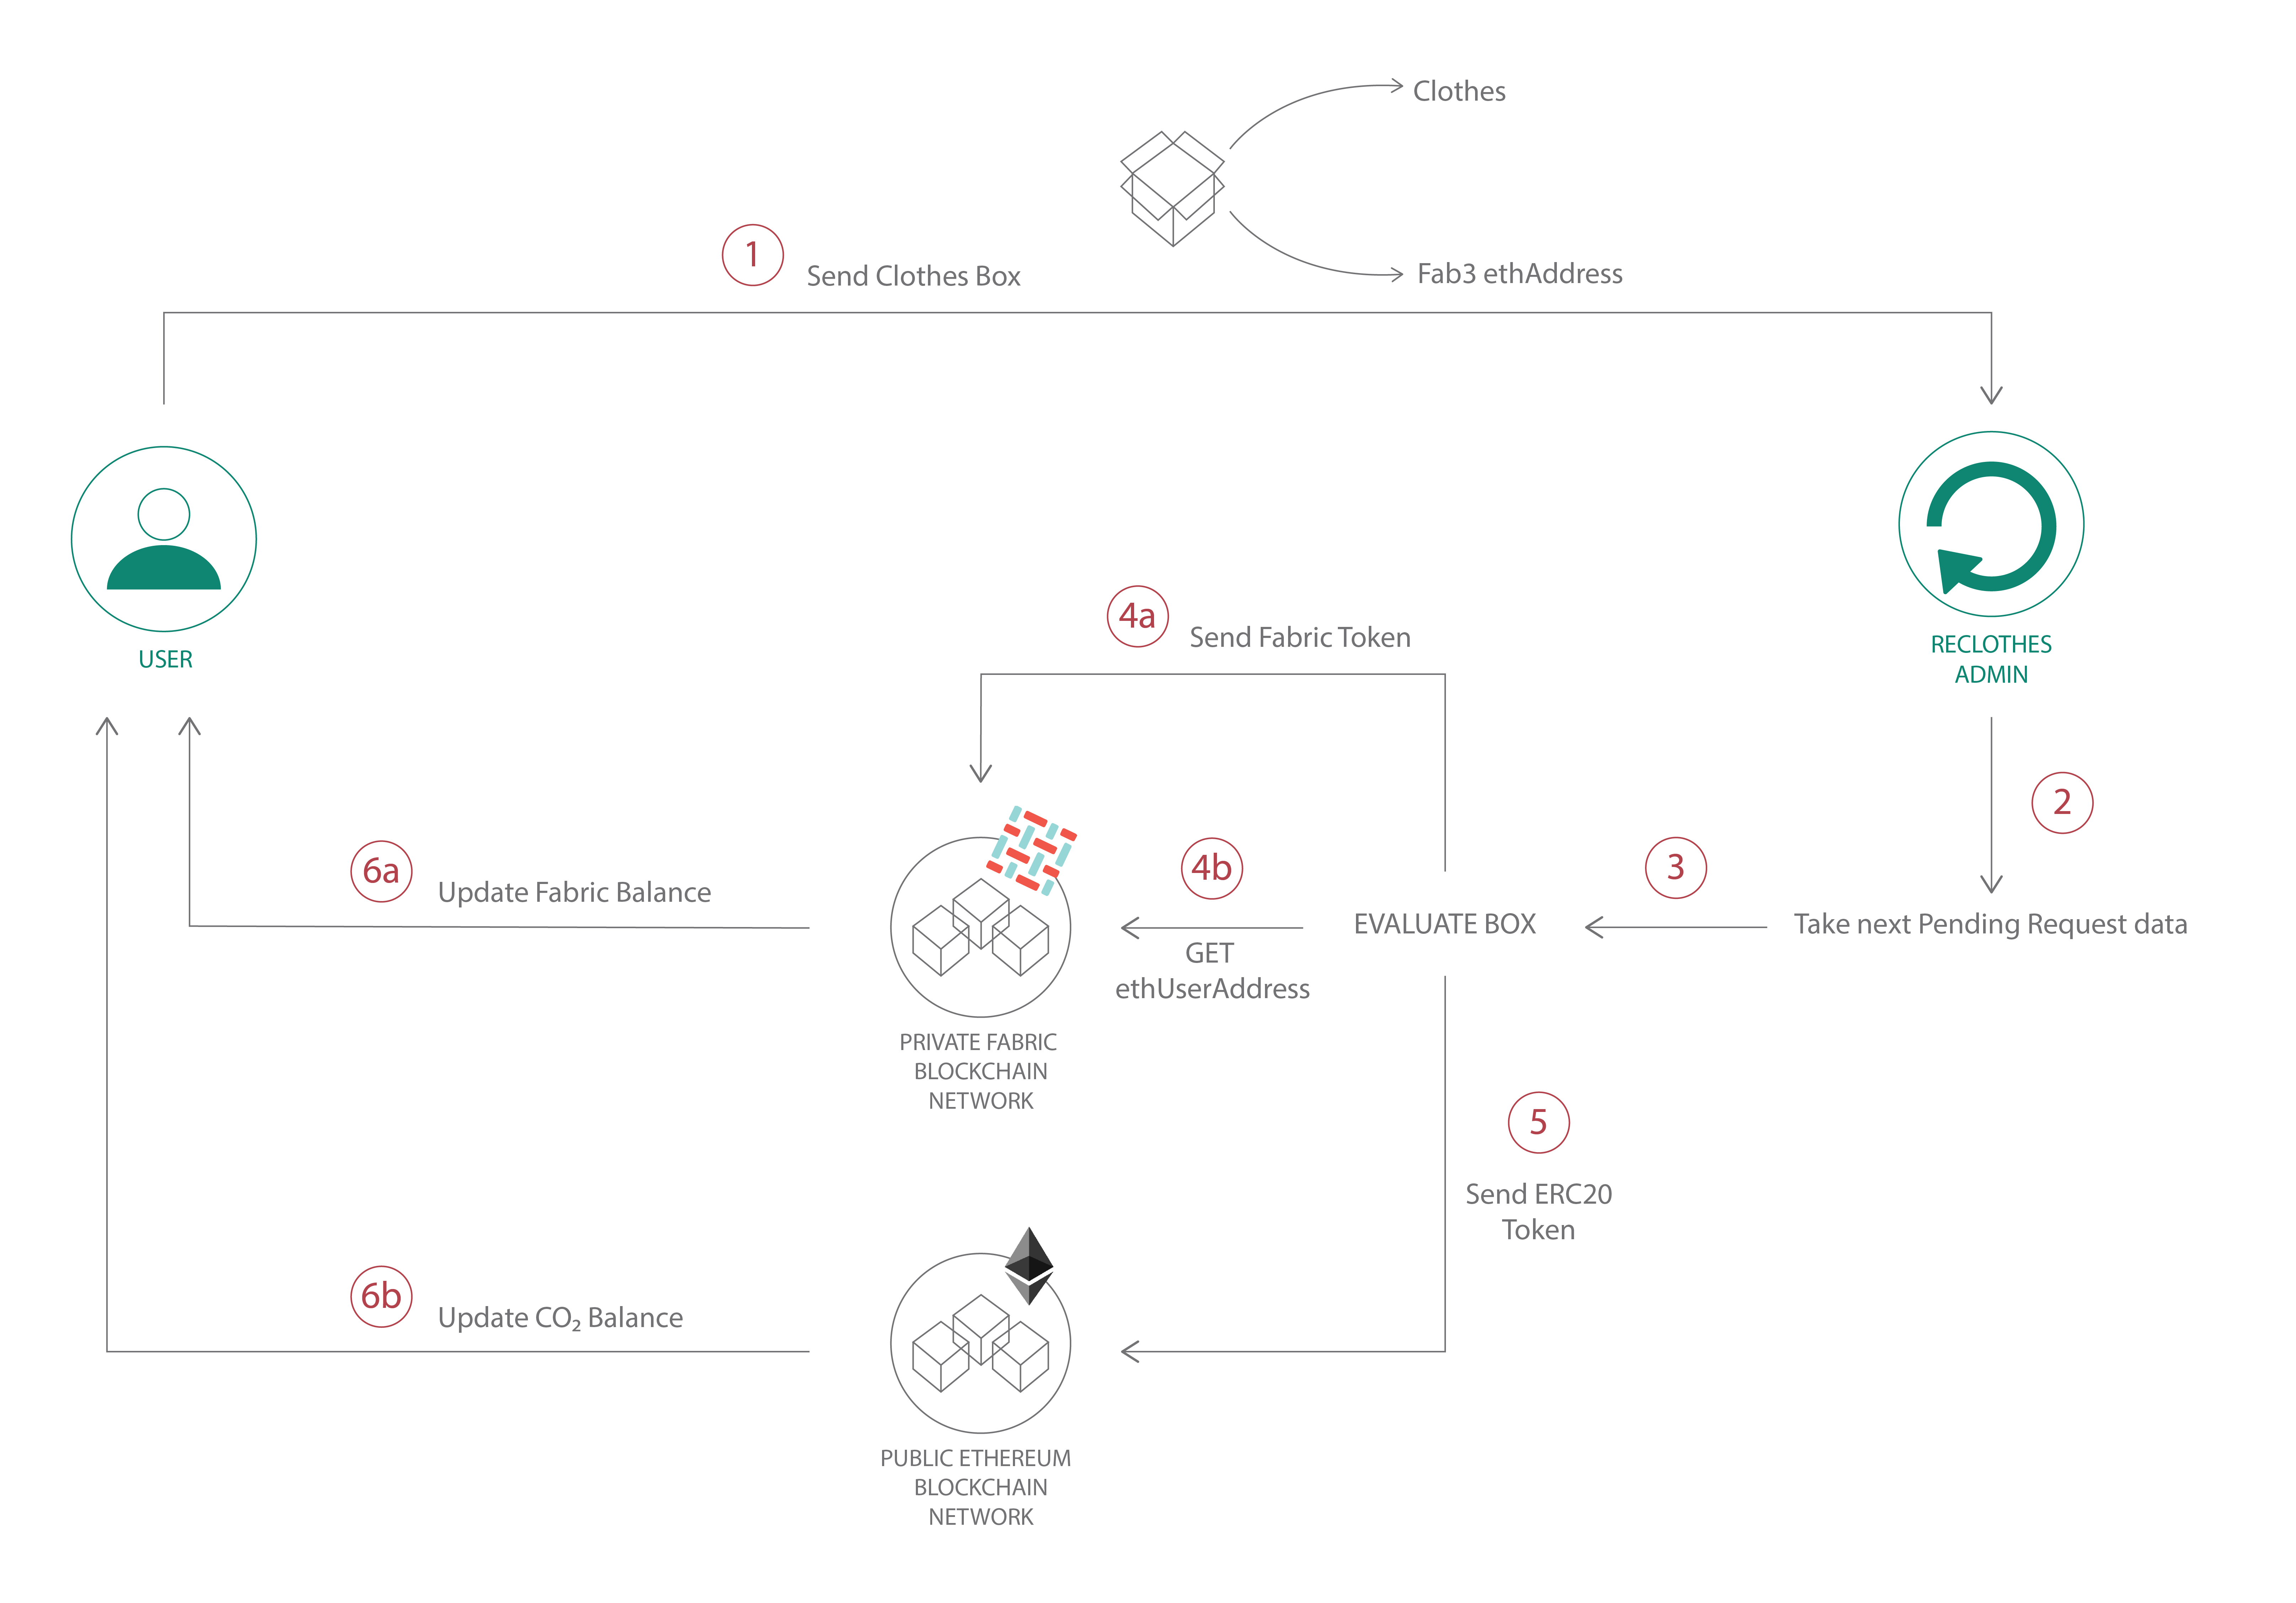
\includegraphics[totalheight=10cm]{img/evaluation.png}
	\caption{Evaluation Process}
	\label{fig:evaluation}
\end{figure}

\begin{figure}[h!]
	\centering
	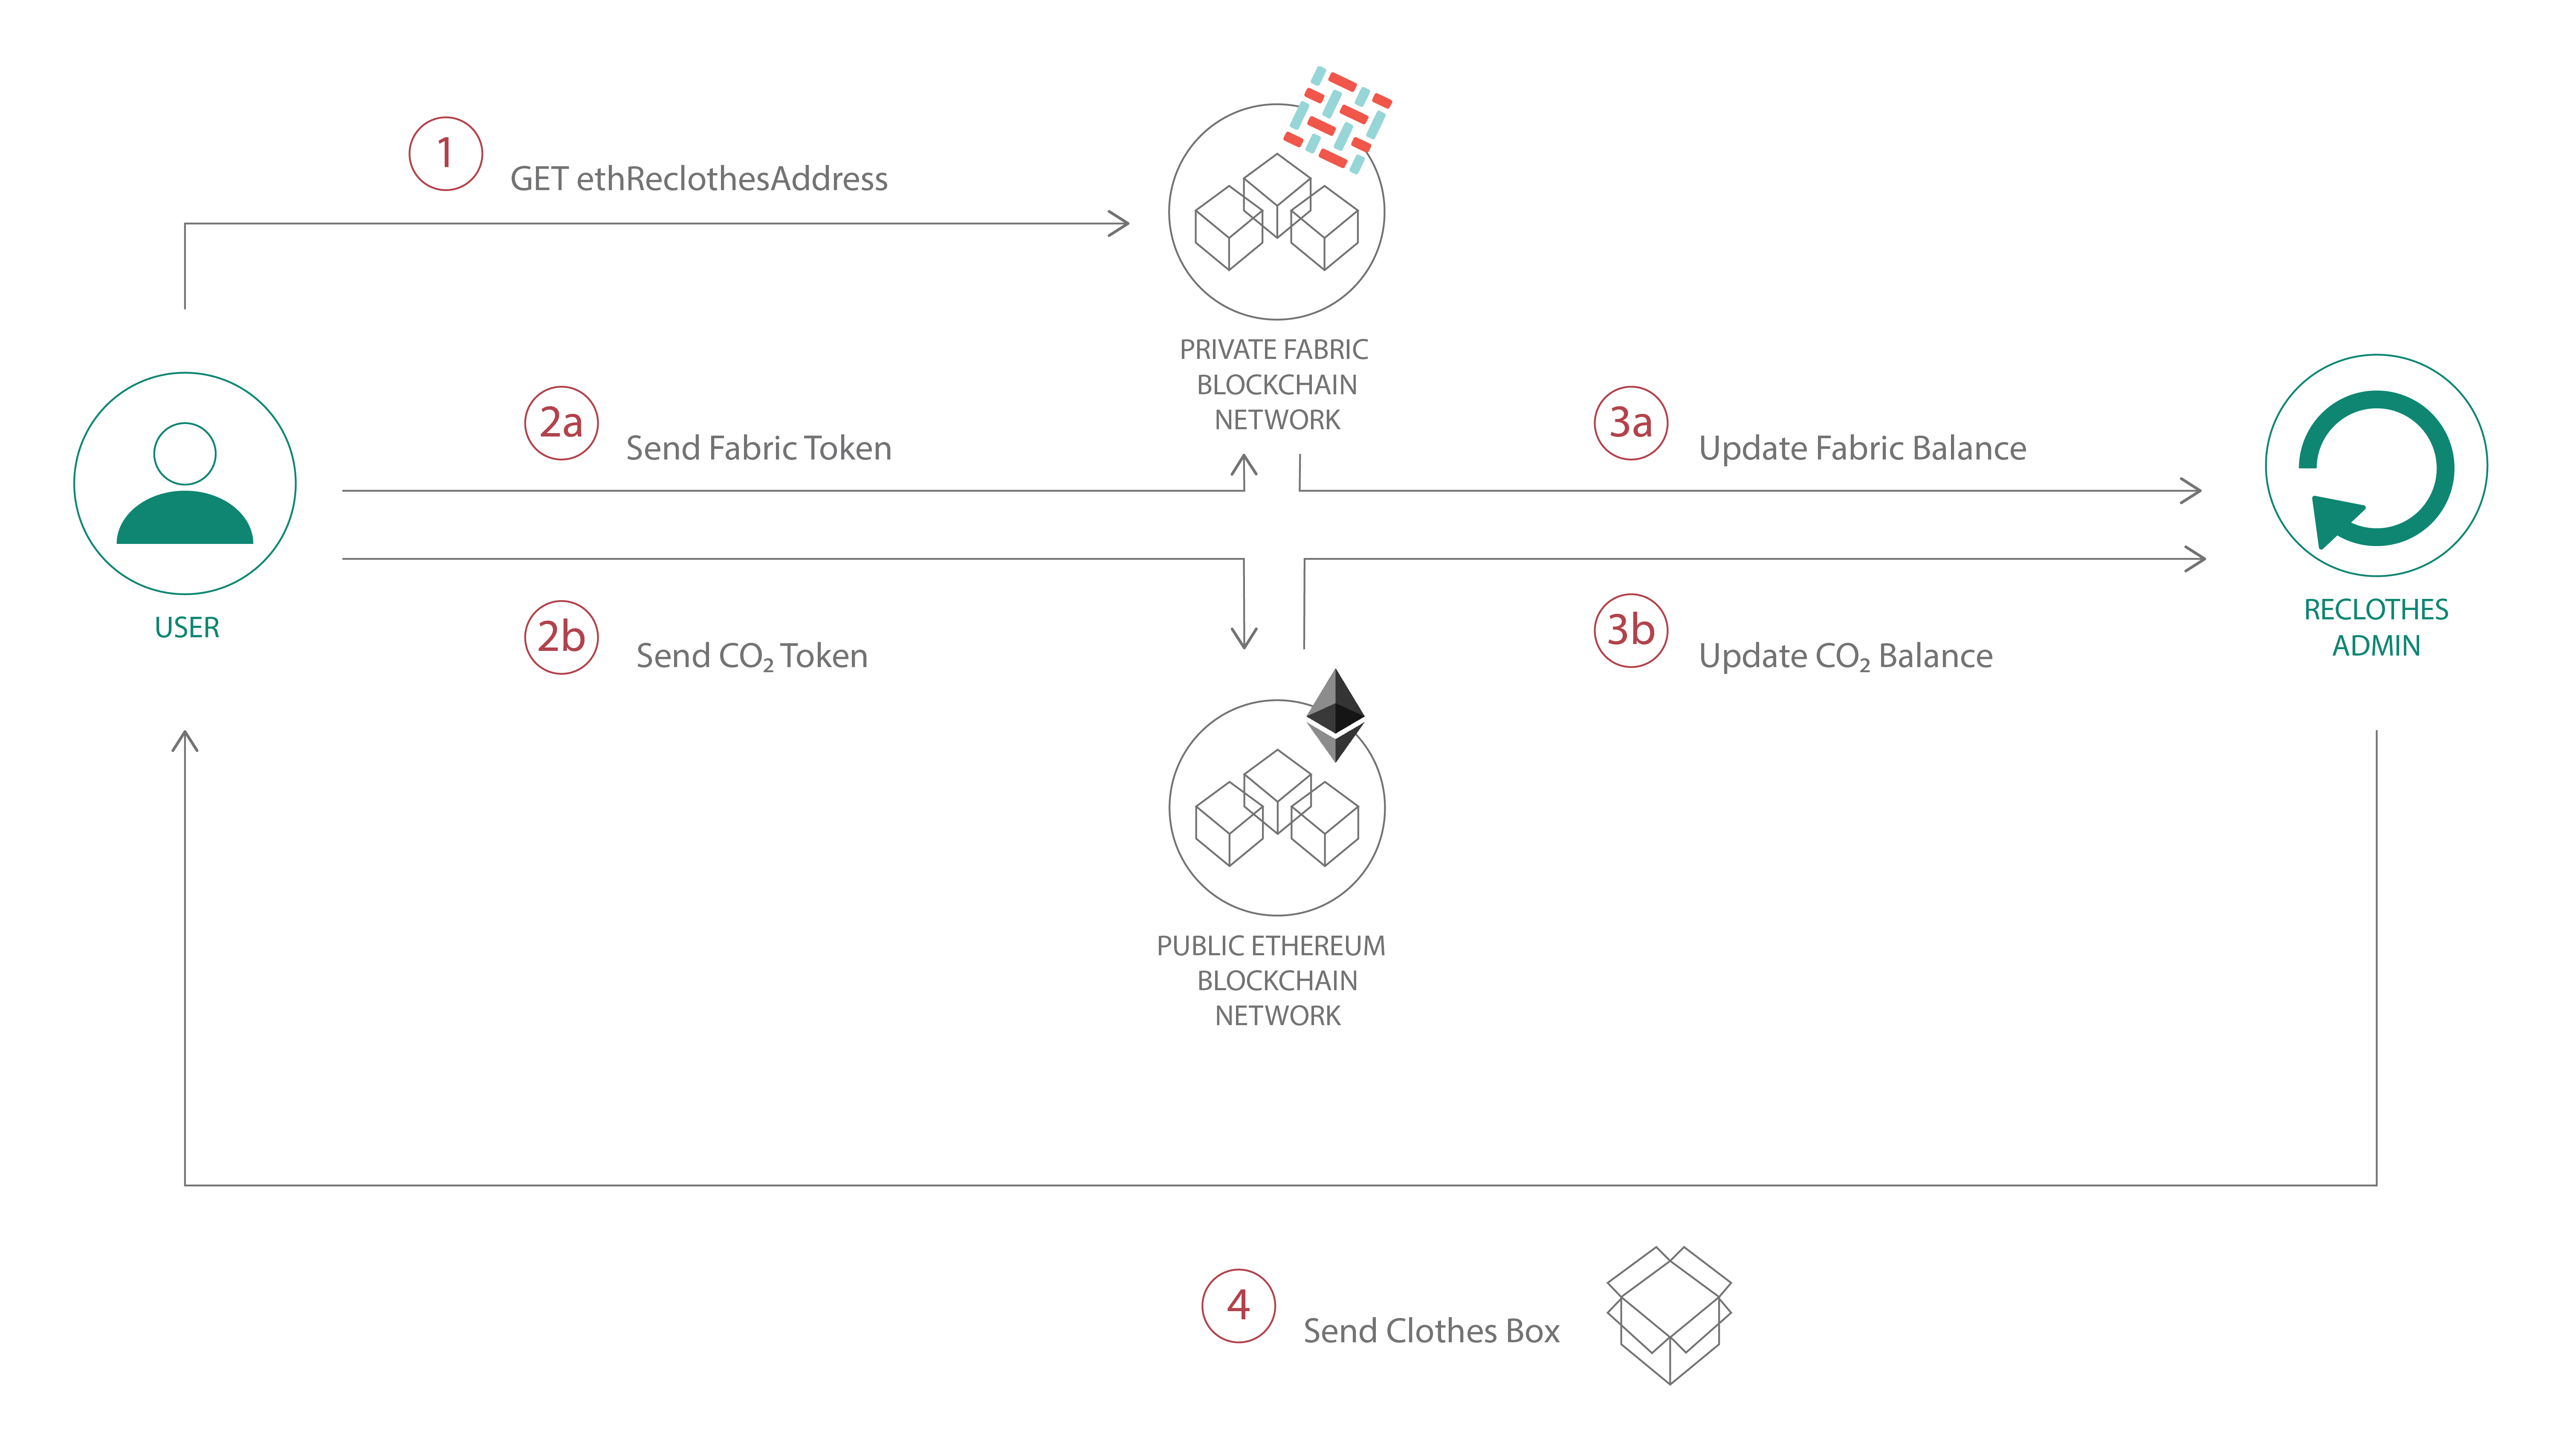
\includegraphics[totalheight=8cm]{img/purchase.png}
	\caption{Purchase Process}
	\label{fig:purchase}
\end{figure}

\clearpage
\subsection{UseCase 2 - Producer Side}

Use case 2 is related to the right side of the overall flow schema shown in Figure \ref{fig:schema}.
It shapes the interactions between Reclothes Admin and Producers. For a better understanding of the 
process involved in that interaction, the use case 2 diagram is shown in \textbf{Figure \ref{fig:usecase2}}.
In that case, all the features are performed over the Hyperledger Fabric network, so there is not a cross-chain 
part. The token exchanged, \texttt{Regeneration Credit}, is based over Fabric smart contract and it is point-based, 
without the need to involve the Ethereum blockchain.

\bigskip 
Analyzing Figure \ref{fig:usecase2}, even here, there is the main action that leads to a transaction process. 
Looking at the diagram we could split the flow into two sub-flow, the first one from Reclothes to Producer. In 
that sub-flow we could identify two main actions \textbf{\texttt{\textit{Send Box}}} and 
\textbf{\texttt{\textit{Purchase Box}}}.  As specified in the previous use case, these is the operation that 
performs a world state update of the blockchain ledger. On the other hand, in the second sub-flow, from Producer 
to Reclothes, just one action that produces an outgoing token transfer is involved, the 
\textbf{\texttt{\textit{Evaluate Material}}} function. 

\bigskip 
All the assets exchanged are handled using \textbf{Regeneration Credits}. It is a Fabric token exchanged and 
handled by the Fabric chaincode, it runs over Fabric network. To test the use case I consider just one 
Producer that performs the overall recycling process, even if the smart contract is structured in order to 
allow the handling and management of more Producer actors involved in the system. In the case of many Producers 
involved in the recycling process, an ERC20 integration to handle the Regeneration
Credits exchanged can be an improvement. Moreover, that change will not have a strict correlation 
between credits and Reclothes. It allows the Producers to use the token to handle the internal process with 
more clients. 


\begin{outline}[enumerate]
    \1 \textbf{from Reclothes to Producer}   
    \2 \textbf{Send Box}
    \3 The Reclothes Admin after has performed the filtering process over the clothes box received by the Users. 
    Then all the clothes in a bad status, that could not be resold inside the platform store, are sent to the 
    Producer in order to recycle the material and produce upcycled clothes. The Admin performs the Send Box 
    operation, like the Send Box performed in the use case 1, it contains the same data inside the request 
    (\texttt{t-shirt, pants, jacket, other} with the related number of items). The box is sent to the Producer 
    Company. In the case of more Producers, the send box request includes the selected Producer Company chosen.
    \3 Once the Producer performed the \textit{\texttt{Evaluation}} process over the sent clothes box, 
    The Reclothes Account gain the corresponding amount of \textbf{Regeneration Credits} based on the 
    old materials evaluation. Once that the balance is updated, the Reclothes Admin can spend that 
    credits to purchase items. 
    
    \2 \textbf{Purchase Box}
    \3 Reclothes Admin can purchase boxes by the Producer Company with inside clothes realized with recycled 
    materials. At the moment the application allows to purchase three boxes options: 
    \4 \textit{Small Box: 5 items for 50 Regeneration Credits.}
    \4 \textit{Medium Box: 15 items for 150 Regeneration Credits.} 
    \4 \textit{Big Box: 40 items for 200 Regeneration Credits.}

    \3 Once that the Reclothes Admin chooses the box size to purchase, the transaction process starts and the 
    chaincode is invoked. Before is performed a previous check, to control if the Reclothes's wallet, containing the 
    Regeneration Credits, is enough. Then is invoked the transfer method of the smart contract, the Regeneration Credits are 
    redeemed to the Producer account and the shipping of the Box start, with inside the recycled clothes.       

    \1 \textbf{from Producer to Reclothes}
    \2 \textbf{Evaluate Material}
    \3 Once the box sent by the Reclothes Admin arrives, it must be evaluated. The Evaluation process
    consists to evaluate all the materials related to the clothes received. To obtain a standard evaluation
    there is a reference table listing a fixed amount of Regeneration Credits provided for
    each clothes based on \textit{material} and \textit{weight}. Once the Producer Admin performed 
    the evaluation of the materials for each clothes, and the total amount of Regeneration Credit is fixed,
    the transaction process starts. The chaincode is invoked and the transaction is performed from Producer account
    to Reclothes account over Fabric network. Producer side, there are two parameters to analyze:
    \4 \textbf{Regeneration Credits Supplied}: It is the total amount of credits emitted over the time.
    \4 \textbf{Regeneration Credits Circulating}: It is the amount of credits that Reclothes Admin
    owns and could spend for purchasing. 
\end{outline}


\begin{figure}[h!]
	\centering
	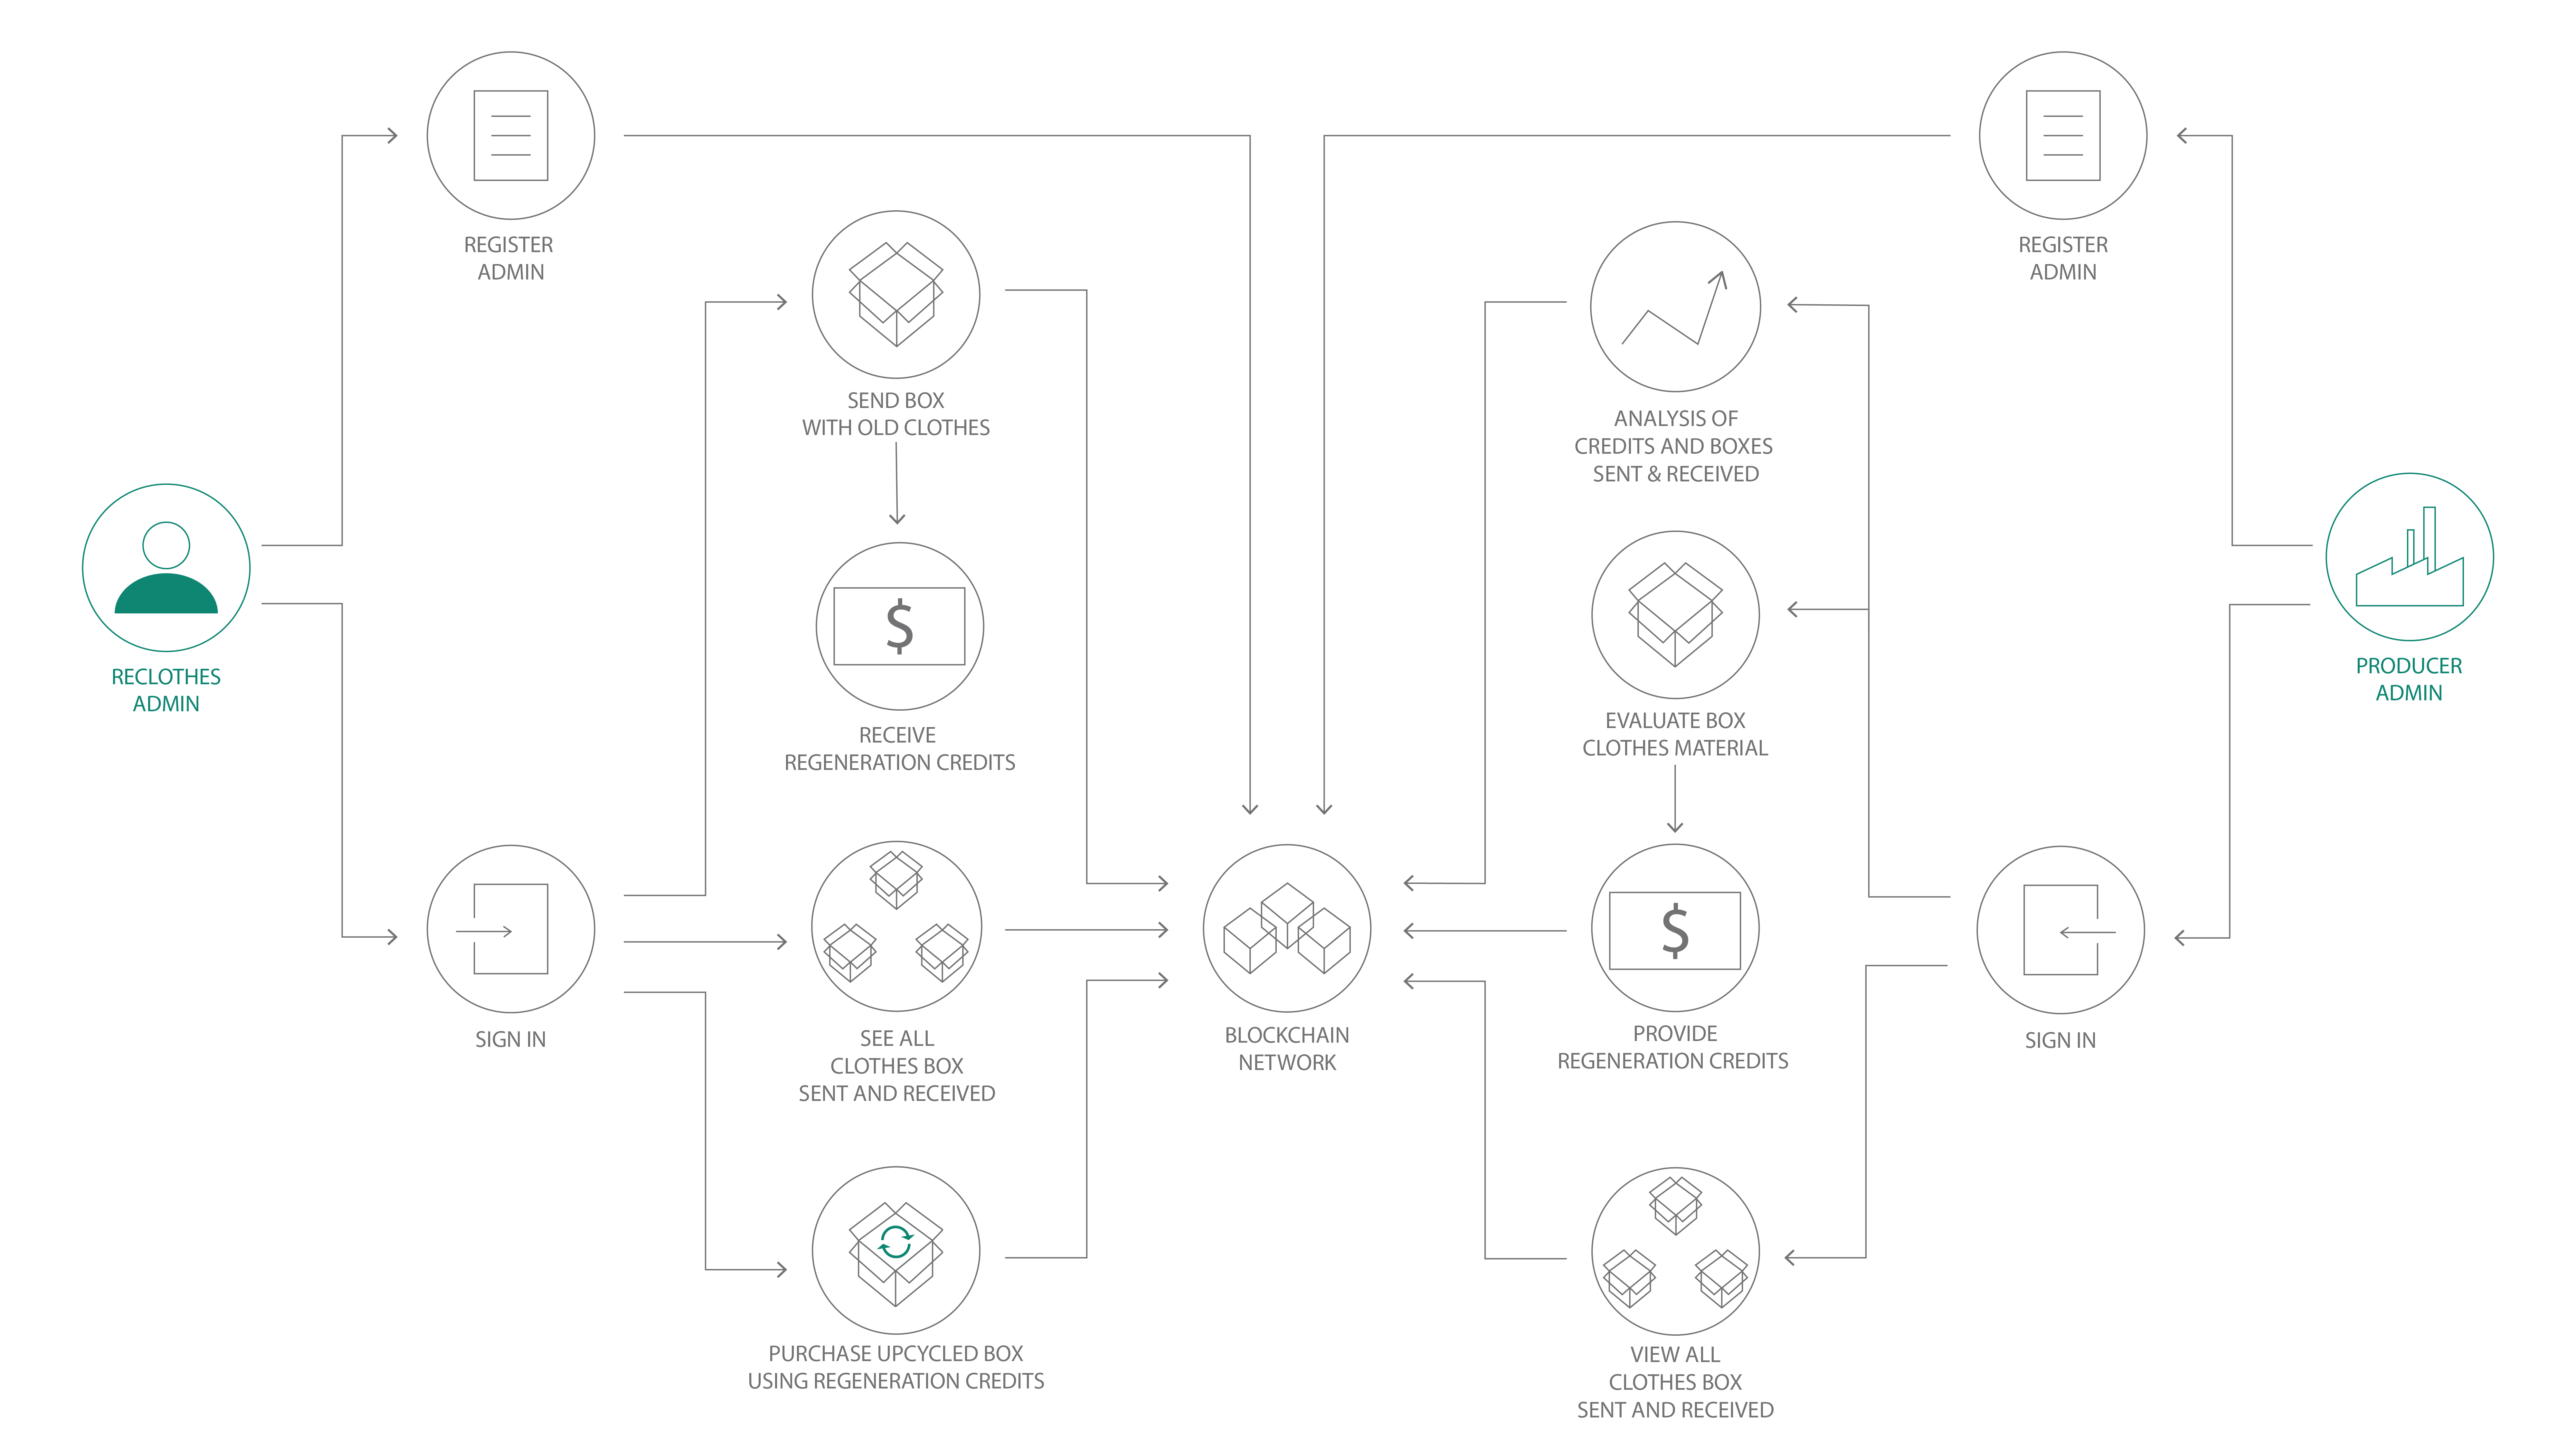
\includegraphics[totalheight=10cm]{img/use_case2.png}
	\caption{UseCase 2}
	\label{fig:usecase2}
\end{figure}


%SMART CONTRACT
\newpage
\section{Smart Contract}

For the smart contract developments I exploited the \texttt{fabric-chaincode-evm}\footnote{To run Solidity Contract over 
Fabric Network, it's used \texttt{fabric-chaincode-evm}\cite{evm-chaincode}, it is an Ethereum virtual machine chaincode developed by IBM 
developers. To allows the integrations there is the need for additional components such as Fab3 Proxy}, it allows us 
to run Ethereum smart contract bytecode inside an Hyperledger Fabric peer. Therefore EVM chaincode bring us to the 
development of the smart contract in Solidity or Vyper programming languages. 
\bigskip

For the development it is used \textbf{Remix}\cite{remix}, it is an online
editor that allows us to write and compile Solidity smart contracts code, providing all the Solidity 
version compiler. Once that the smart contract code is written and the \texttt{.sol} file is produced, 
the compiling process produces two files mandatory for the deployment and uses of the smart contract over 
Fabric network. 
The two file produced are: 
\begin{outline}
    \1 \textbf{ABI}: The \textit{Application Binary Interface} is the standard way to interact with contracts 
    in the Ethereum ecosystem, both from outside the blockchain and for contract-to-contract interaction. The 
    ABI is a .json file that describes the deployed contract and its functions. It allows us to contextualize 
    the contract and call its functions. In other words, the ABI is the description of the contract interface. 
    It contains no code and cannot be run by itself. It is mandatory for smart contract use because the bytecode 
    is the executable EVM code, but by itself, it is without context.

    \1 \textbf{Bytecode}: This is the code that is stored on-chain that describes a smart contract. 
    This code does not include the constructor logic or constructor parameters of a contract. 
    It is a hexadecimal representation of the final contract. It uses the ABI to find the 
    context of the behind contract logic. 
\end{outline}

\bigskip

In order to handle the overall system, three Solidity smart contracts have been developed. Two of them run over the Hyperledger 
Fabric network, exploiting the membership mechanism to access of the chaincode.
In other words, the permission mechanism behind the logic is performed in both networks and chaincode side. 
The network side filters, at the certificate layer, the access to the network. On the other hand, the registration 
mechanism implemented over the chaincode filter the user logged to the network. 
\bigskip

The third smart contract has been developed to run over the Ethereum network. For my thesis work it is used the Ropsten 
testnet. The access to the contract, in that case, is provided by the contract address generated during the deployment 
phase. 
\bigskip

For a better view, below are reported all the contracts involved in the system:
\begin{outline}[enumerate]
    \1 \textbf{Hyperledger Fabric}
    \2 \textbf{User Contract}: It handles the User side, registration, and interaction phase. That contract shapes 
    the use case 1 functionalities. There are the dedicated data structures that care about storing data of actors 
    involved( \texttt{User} and \texttt{Admin} ). It provides a set of getter and setter methods and it has a couple 
    of functions that lead to a transaction process.    
    \2 \textbf{Producer Contract}: It handles the interaction from Reclothes to Producers. That contract shapes the 
    use case 2 behaviors. There are the dedicated data structures that care about storing data of actors  
    involved( \texttt{Admin} and \texttt{Producer} ). It provides a set of getter and setter methods and it includes 
    a couple of function that leads to a transaction process.  

    \1 \textbf{Ethereum}
    \2 \textbf{ERC20 Contract}: It is a standard smart contract with a max Supply fixed to 1,000,000,000.
    The contract is structured following the ERC20 standard. It is not strictly correlated to the thesis application and
    it is exchangeable among each user that owns an Ethereum wallet. The Contract is deployed over the Ropsten network 
    and is accessible using the public contract address. The access to the contract is performed using an Infura node 
    as Ethereum network endpoint.
\end{outline}

\subsection{User Contract} 

The User Contract contains all the features described in the Hyperledger Fabric side of use case 1. 

\subsubsection{Data Structure}

In that contract all the transaction data, related to the points and clothes box transactions, are stored. Moreover, 
the information related to the actors involved in the system, are stored too. 
Thanks to the registration phase, the contract can perform an additional check over the actors that are logged in 
over the Fabric network. The address specified during the registration phase (\texttt{msg.sender}) is the Ethereum 
address generated on the fly by Fab3 Proxy. In the following sections, there is a better and deeper explanation of 
the Fab proxy module and how it works.  
\bigskip

The model of the data structures is divided into 4 structs:

\begin{outline}[enumerate]
    \1 \textbf{User}: model all users data.
    \1 \textbf{Admin}: model Reclothes Admin data.
    \1 \textbf{PointsTransaction}: Model transactions data and incorporate \texttt{TransactionType}, it is used to identify the flows direction.
    \1 \textbf{ClothesBox}: The box sent with old clothes .
\end{outline}

\begin{lstlisting}[language=Solidity]
       
    // model a user
        struct User {
            address userAddress;    // User address (inside fabric environment)
            address publicAddress;  // external eth public address of User Admin
            string firstName;
            string lastName;
            string email;
            uint points;            // Fabric points amount
            bool isRegistered;      // Flag for internal use
            uint numTransaction;    // number of transactions performed
            mapping(uint => PointsTransaction) userTransactions;
            uint numBox;            // number of box transaction evaluated
            mapping(uint => ClothesBox) box;
        }
    
        // model a admin
        struct Admin {
            address adminAddress;   // Admin address (inside fabric environment)
            address publicAddress;  // external eth public address of Admin
            string name;
            bool isRegistered;      // Flag for internal use
        }
    
        // model points transaction
        enum TransactionType { Earned, Redeemed }
        struct PointsTransaction {
            uint points;
            TransactionType transactionType;
            address userAddress;    // user address involved
            address adminAddress;   // admin address involved
        }
    
        // model clothes box to ship
        struct ClothesBox {
            address userAddress; // reclothes-producer Admin
            uint tshirt;        // Number of item
            uint pants;         // Number of item
            uint jacket;        // Number of item
            uint other;         // Number of item
            bool isEvaluated;   // Flag to check if box evaluation is performed
            uint points;        // fabric value amount of the box
        }
\end{lstlisting}

\subsubsection{Getter}
The User Contract allows access to a set of methods, to obtain information about the system status.
Once the user is logged in as User or Admin, it could perform part of that getter invocation.
Parts of the method are developed for internal usage, the other ones are dedicated to providing to the actor's 
information about the system, or it is useful to start other invocations dapp side. Access to some method is 
handled using the modifier method that performs a filtering process of the function caller. 
\bigskip 

\begin{lstlisting}[language=Solidity]
    
    /***********************************************/
    /***************** Users Data ******************/
    /***********************************************/
                           ....
                           ....

    /****************************************************/
    /*** All Box Requests -> Old, Evaluated, UpCycled ***/
    /****************************************************/

    //Get PendingBox by index
    function getPendingRequest(uint _pendingIndex) public view returns(address, uint, uint, uint, uint, bool, uint) {
        // only admin can call
        require(admins[msg.sender].isRegistered, "Admin address not found");

        //check index
        require(_pendingIndex<pendingIndex, "Wrong index");

        return (pendingBox[_pendingIndex].userAddress, pendingBox[_pendingIndex].tshirt, pendingBox[_pendingIndex].pants, pendingBox[_pendingIndex].jacket, pendingBox[_pendingIndex].other, pendingBox[_pendingIndex].isEvaluated, pendingBox[_pendingIndex].points);
    }

    //Get EvaluatedBox by index
    function getEvaluatedRequest(uint _evaluatedIndex) public view returns(address, uint, uint, uint, uint, bool, uint) {
        // only admin can call
        require(admins[msg.sender].isRegistered, "Admin address not found");

        //check index
        require(_evaluatedIndex<evaluatedIndex, "Wrong index");

        return (evaluatedBox[_evaluatedIndex].userAddress, evaluatedBox[_evaluatedIndex].tshirt, evaluatedBox[_evaluatedIndex].pants, evaluatedBox[_evaluatedIndex].jacket, evaluatedBox[_evaluatedIndex].other, evaluatedBox[_evaluatedIndex].isEvaluated, evaluatedBox[_evaluatedIndex].points);
    }

    function getTransactionInfo(uint _transactionIndex) onlyUser(msg.sender) public view returns(uint, uint, address, address) {
        //require index exists
        require(users[msg.sender].numTransaction > _transactionIndex && _transactionIndex >= 0, "Wrong transaction index");

        return (users[msg.sender].userTransactions[_transactionIndex].points, uint(users[msg.sender].userTransactions[_transactionIndex].transactionType), users[msg.sender].userTransactions[_transactionIndex].userAddress, users[msg.sender].userTransactions[_transactionIndex].adminAddress);
    }
                            ....
                            ....

\end{lstlisting}

\subsubsection{Transactions}

The transactions process is the main process of the overall smart contract. This method performs a
write access to the smart contract and modifies  the world state of the ledger stored over the Fabric blockchains peers. 
\bigskip 

There are two functions that perform transactions between actors involved in the smart contracts,
these are :

\begin{outline}[enumerate]
    \1 \textbf{earnPoints}: It is an internal function called by \texttt{EvaluateBox}.
    Once that user performed the \texttt{sendBox} process, Admin side, starts the evaluation process.
    Therefore the Admin evaluates the pending request and sets a total amount of points related to 
    the box received. Then the \texttt{EvaluateBox} function call the internal function \texttt{earnPoints}
    passing as argument the amount to be transfer and the userAddress of the clothes box sender. Then
    the function performs the Fabric points transaction from Reclothes to User.
    
     \1 \textbf{usePoints}: It is related to the purchase process. When the User performs a purchase over
     the platform store, there is the calculation of the overall amount related to the items purchased, and internally
     is invoked the \texttt{usePoints} function. That function after a set of previous checks, then 
     decrease the User balance of the related amount passed to the function.
\end{outline}

\begin{lstlisting}[language=Solidity]
    
    /****************************************************/
    /************* Transactions Operations **************/
    /****************************************************/

    //update users with points earned
    function earnPoints (uint _points, address _userAddress ) onlyAdmin(msg.sender) internal {

      // verify user address
      require(users[_userAddress].isRegistered, "User address not found");

      // update user account
      users[_userAddress].points = users[_userAddress].points + _points;

      PointsTransaction memory earnTx = PointsTransaction({
        points: _points,
        transactionType: TransactionType.Earned,
        userAddress: _userAddress,
        adminAddress: admins[msg.sender].adminAddress
      });

      // add transaction
      transactionsInfo.push(earnTx);

      users[_userAddress].userTransactions[users[_userAddress].numTransaction] = earnTx;
      users[_userAddress].numTransaction++;

      usersTransactions[totTx] = earnTx;
      totTx++;

    }

    //Update users with points used
    function usePoints (uint _points) onlyUser(msg.sender) public {

      // verify enough points for user
      require(users[msg.sender].points >= _points, "Insufficient points");

      // update user account
      users[msg.sender].points = users[msg.sender].points - _points;

      PointsTransaction memory spendTx = PointsTransaction({
        points: _points,
        transactionType: TransactionType.Redeemed,
        userAddress: users[msg.sender].userAddress,
        adminAddress: 0
      });

      // add transaction
      transactionsInfo.push(spendTx);

      users[msg.sender].userTransactions[users[msg.sender].numTransaction] = spendTx;
      users[msg.sender].numTransaction++;

      usersTransactions[totTx] = spendTx;
      totTx++;
    }

    /****************************************************/
    /************** Clothes Box Operations **************/
    /****************************************************/

    //handle box
    function sendBox(uint _tshirt, uint _pants, uint _jackets, uint _other) onlyUser(msg.sender) public {

         pendingBox[pendingIndex] = ClothesBox({
             userAddress: msg.sender,
             tshirt: _tshirt,
             pants: _pants,
             jacket: _jackets,
             other: _other,
             isEvaluated: false,
             points: 0
         });

         users[msg.sender].box[users[msg.sender].numBox] = pendingBox[pendingIndex];

         users[msg.sender].numBox++;
         pendingIndex++;
    }

    //evaluate box
    function evaluateBox(uint _points) onlyAdmin(msg.sender) public {
        //check correct pending request index
        require(evaluatedIndex < pendingIndex, "No more pending request");

        //check if evaluation is done
        require(!pendingBox[evaluatedIndex].isEvaluated, "Request just evaluated");

        //pop pending request
        ClothesBox storage box = pendingBox[evaluatedIndex];

        //update box transaction
        box.isEvaluated = true;
        box.points = _points;

        //send points to the userAddress
        earnPoints(_points, box.userAddress);

        //add evaluated box
        evaluatedBox[evaluatedIndex] = box;
        evaluatedIndex++;
    }

    //get user balance
    function getBalance() public view returns (uint) {
        return users[msg.sender].points;
    }
\end{lstlisting}

%% producer contract 
\subsection{Producer Contract}

The Producer Contract contains all the features described in the use case 2 diagram shown in 
the Figure \ref{fig:usecase2}.

\subsubsection{Data Structure}

In that contract, all the transaction data related to the points and clothes box transactions, are stored. Moreover, 
the information related to the actors involved in the system are stored; in this case, the actors involved are 
the \texttt{Admin} and the \texttt{Producer}.
As the previous contract, the registration phase provides an additional check over the actors logged in over the 
Fabric network. The address specified during the registration phase (\texttt{msg.sender}) is always the Ethereum 
address generated on the fly by Fab3 Proxy.
\bigskip

Briefly explaining the behavior of the relationship among contracts. The Fab3 proxy has a 1 to 1 association 
instance/user. There is the possibility that the Admin logged and registered, over \texttt{UserContract}, associated 
with one Fab3 instance, set over the channel that communicates with \texttt{UserContract}, must perform another 
registration with a new Fab3 proxy instance, in order to set the communication with the channel dedicated for 
\texttt{ProducerContract}. It means that for each Fab3 instance there is a new Eth address generated and the Admin 
could have two Ethereum addresses, one associated with \texttt{UserContract} and the other one associated with 
\texttt{PrducerContract}.
\bigskip


The model of the data structures is divided into 3 structs:

\begin{outline}[enumerate]
    \1 \textbf{Producer}: model all Producers data.
    \1 \textbf{Admin}: model Reclothes Admin data.
    \1 \textbf{ClothesBox}: The box sent with old clothes.
\end{outline}

\begin{lstlisting}[language=Solidity]
    // model a producer
    struct Producer {
        address adminAddress;   // Producer Admin address (inside fabric environment)
        address publicAddress;  // external eth public address of Producer Admin
        string name;            // Producer admin name
        bool isRegistered;      // Flag for internal use
        uint numBox;            // number of box transactions evaluated
        uint pointsProvided;    // amount of points provided by own evaluations
        mapping(uint => ClothesBox) box;
    }

    // model a admin
    struct Admin {
        address adminAddress;   // Admin address (inside fabric environment)
        address publicAddress;  // external eth public address of Admin
        string name;            // Admin name
        bool isRegistered;      // Flag for internal use
        uint numBox;            // number of box transaction evaluated
        uint creditSpent;       // amount of points provided by own evaluations
        mapping(uint => ClothesBox) box;
    }

    struct ClothesBox {
        address adminAddress; // reclothes-producer Admin
        uint tshirt;        // Number of item
        uint pants;         // Number of item
        uint jacket;        // Number of item
        uint other;         // Number of item
        bool isEvaluated;   // Flag to check if box evaluation is performed
        uint points;        // fabric value amount of the box

        //mapping(uint => Clothes) clothes;
    }
\end{lstlisting}

\subsubsection{Getter}

The Producer Contract allows access to a set of method to get information about the system status.
Once the user is logged in as Admin or Producer, he can performs part of that getter invocation.
Parts of the method are developed for internal usage, the other ones are dedicated to provide to the actor's 
information about the system, or it is useful to start other invocations dapp side. Access to some method is 
handled using the modifier method that performs a filtering process of the function caller.
\bigskip 

Below I reported only the main smart contract methods.
\bigskip

\begin{lstlisting}[language=Solidity]
   
    /****************************************************/
    /*** All Box Requests -> Old, Evaluated, UpCycled ***/
    /****************************************************/

    function getPendingRequest(uint _pendingIndex) public view returns(address, uint, uint, uint, uint, bool, uint) {
        //check index
        require(_pendingIndex<pendingIndex && _pendingIndex>=0, "Wrong index");

        return (pendingBox[_pendingIndex].adminAddress, pendingBox[_pendingIndex].tshirt, pendingBox[_pendingIndex].pants, pendingBox[_pendingIndex].jacket, pendingBox[_pendingIndex].other, pendingBox[_pendingIndex].isEvaluated, pendingBox[_pendingIndex].points);
    }

    function getNextPendingRequest() public view returns(address, uint, uint, uint, uint, bool, uint) {
        //check index
        require(evaluatedIndex<pendingIndex, "No More Pending Request");

        return (pendingBox[evaluatedIndex].adminAddress, pendingBox[evaluatedIndex].tshirt, pendingBox[evaluatedIndex].pants, pendingBox[evaluatedIndex].jacket, pendingBox[evaluatedIndex].other, pendingBox[evaluatedIndex].isEvaluated, pendingBox[evaluatedIndex].points);
    }


    /********* Evaluated Request -> Box with Old Clothes evaluated *********/
    function getEvaluatedRequest(uint _evaluatedIndex) public view returns(address, uint, uint, uint, uint, bool, uint) {
        //check index
        require(_evaluatedIndex<evaluatedIndex && upCycledIndex>=0, "Wrong index");

        return (evaluatedBox[_evaluatedIndex].adminAddress, evaluatedBox[_evaluatedIndex].tshirt, evaluatedBox[_evaluatedIndex].pants, evaluatedBox[_evaluatedIndex].jacket, evaluatedBox[_evaluatedIndex].other, evaluatedBox[_evaluatedIndex].isEvaluated, evaluatedBox[_evaluatedIndex].points);
    }


    /********* UpCycled Request -> Box with New Clothes *********/
    function getUpCycledRequest(uint _upCycledIndex) public view returns(address, uint, uint, uint, uint, bool, uint) {
        //check index
        require(_upCycledIndex<upCycledIndex && upCycledIndex>=0, "Wrong index");

        return (upCycledBox[_upCycledIndex].adminAddress, upCycledBox[_upCycledIndex].tshirt, upCycledBox[_upCycledIndex].pants, upCycledBox[_upCycledIndex].jacket, upCycledBox[_upCycledIndex].other, upCycledBox[_upCycledIndex].isEvaluated, upCycledBox[_upCycledIndex].points);
    }

    /****************************************************/
    /***************** Data of Requests *****************/
    /****************************************************/

    function getTotPointsProvided() public view returns(uint) {
        return totPointsProvided;
    }

    function getRegenerationCredit() public view returns(uint) {
        return debtPoints;
    }

    function getTotBoxOld() public view returns(uint) {
        return totBoxOld;
    }

    function getTotBoxNew() public view returns(uint) {
        return totBoxNew;
    }

\end{lstlisting}

\subsubsection{Transactions}

As explained above, transactions process are the main ones of the smart contracts, leading to a write
operation.
\bigskip.

There are two functions that perform transactions between the actors involved in that contract:

\begin{outline}[enumerate]
    \1 \textbf{evaluateBox}: The evaluation process starts by the invocation of \texttt{SendBox} function.
    Once that there are pending box requests, the next one is evaluated following
    the price table in order to standardize clothes materials evaluation by \texttt{material type} and \texttt{weight}.
    It is set an overall amount of value corresponding to the clothes box request.
    The transfer process involves, in the thesis work, just one Producer. The points are 
    handled with a \texttt{debtPoints} variable that is updated by these two functions. In that
    case \texttt{evaluateBox} add the amount value of the box to the \texttt{debtPoints} variable. 

    \1 \textbf{buyUpcycledBox}: This process leads a purchase order performed by the Admin to the 
    Producer. Admin chooses a kind of fixed box(\texttt{small, medium, large}) with a fixed Regeneration
    Credits price associated. Before performing the purchase process, there is a check of the \texttt{debtPoints}
    balance to allow or not the transaction of the box. If the amount of the Regeneration Credits
    is enough to buy upcycled clothes, then the \texttt{debtPoints} is updated and the value of the
    purchased box is subtracted to the overall balance. 
\end{outline}

\begin{lstlisting}[language=Solidity]
    
    // Evaluate Old Box
    function evaluateBox(uint _points) onlyProducer() public {
        //check correct pending request index
        require(evaluatedIndex < pendingIndex, "No more pending request");

        //check if evaluation is done
        require(!pendingBox[evaluatedIndex].isEvaluated, "Request just evaluated");

        //pop pending request
        ClothesBox storage box = pendingBox[evaluatedIndex];

        //update box transaction
        box.isEvaluated = true;
        box.points = _points;

        //add evaluated box
        evaluatedBox[evaluatedIndex] = box;
        evaluatedIndex++;

        debtPoints += _points;
        totPointsProvided += _points;
    }

    function buyUpcycledBox(uint _tshirt, uint _pants, uint _jackets, uint _other, uint _points) onlyAdmin() public {
        require(debtPoints >= _points, "Not enought credits accumulated in old material boxes");

        ClothesBox memory box = ClothesBox({
         adminAddress: msg.sender,
         tshirt: _tshirt,
         pants: _pants,
         jacket: _jackets,
         other: _other,
         isEvaluated: true,
         points: _points
        });

        admins[msg.sender].box[admins[msg.sender].numBox] = box;
        admins[msg.sender].numBox++;
        admins[msg.sender].creditSpent += _points;

        //add upcycled box
        upCycledBox[upCycledIndex] = box;
        upCycledIndex++;

        debtPoints -= _points;
        totBoxNew++;
    }

\end{lstlisting}

%% erc20 contract
\subsection{ERC20 Contract}
\label{erc20}

ERC-20 is a technical standard used to issue and implement tokens over the Ethereum blockchain.
The standard describes a common set of rules that should be followed for a token to function properly
within the Ethereum ecosystem. Therefore, ERC-20 should not be considered as a piece of code or 
software. Instead, it may be described as a technical guideline or specification.
\bigskip

The choice to develop an ERC-20 token leads to relaxing the limitation related to the token usage. That 
contract is deployed over the Ethereum network and it is public, accessible to everyone that owns an Ethereum 
wallet. The decision, as well as a cross-chain interaction process, leads to open the doors to an external usage 
of the token, due to what the asset represents
\bigskip

The asset wants to represent the CO\textsubscript{2} emission saved. For example, as asset exchange to measure 
the emission saved recycling a t-shirt even to produce it starting from scratch.
\bigskip

The main information associated to the created token are: 

\begin{outline}
    \1 \textbf{Symbol}: CO2, it is used to identify a token, this is a three or four letter abbreviation of the token.
    \1 \textbf{Name}: CarbonToken, it able to identify them.
    \1 \textbf{Total supply}: 1,000,000,000, it is the max supply of the token.
    \1 \textbf{Decimals}: 18, it is used to determine what decimal place the amount of the token will be calculated. 
    The most common number of decimals to consider is 18. 
\end{outline}

The main features of the contract are describer by ERC20 interface

\begin{lstlisting}[language=Solidity]
    contract ERC20Interface {
        function totalSupply() public constant returns (uint);
        function balanceOf(address tokenOwner) public constant returns (uint balance);
        function allowance(address tokenOwner, address spender) public constant returns (uint remaining);
        function transfer(address to, uint tokens) public returns (bool success);
        function approve(address spender, uint tokens) public returns (bool success);
        function transferFrom(address from, address to, uint tokens) public returns (bool success);
    
        event Transfer(address indexed from, address indexed to, uint tokens);
        event Approval(address indexed tokenOwner, address indexed spender, uint tokens);
    }
\end{lstlisting}

\bigskip

Below I list and explain in details the six mandatory functions that defines the erc20 tokens:

\begin{outline}
    \1 \textbf{totalSupply()}: the supply could easily be fixed, as it happens with Bitcoin, this function 
    allows an instance of the contract to calculate and return the total amount of the token that exists 
    in circulation.
    \1 \textbf{balanceOf()}: This function allows a smart contract to store and return the balance of 
    the provided address. The function accepts an address as a parameter, so it should be known that 
    the balance of any address is public.
    \1 \textbf{approve()}: When calling this function, the owner of the contract authorizes, or approves, 
    the given address to withdraw instances of the token from the owner’s address.
    \1 \textbf{transfer()}: This function lets the owner of the contract send a given amount of the token 
    to another address just like a conventional cryptocurrencies transaction.
    \1 \textbf{transferFrom()}: This function allows a smart contract to automate the transfer process 
    and send a given amount of the token on behalf of the owner.
    \1 \textbf{allowance()}: This functions allow the caller to check if the given balance's address has 
    enough token to send the amount to an other address.
\end{outline}

% NETWORK
\newpage
\section{Network Architecture}

\subsection{Main Components}

Before going deeper to explain my network architectural choice, it is important to have an overview
of the main components involved in the Hyperledger Fabric Architecture:

\begin{outline}[enumerate]
    \1 \textbf{Peer}: It is the fabric node, there are different kinds of peers and each one can perform
    specific actions
    \2 \textbf{Anchor Peer}: this kind of peer is used for communications between organizations. It makes peers in different organizations aware each other.
    \2 \textbf{Committing Peer}: Every peer in the channel
    \2 \textbf{Endorsing Peer}: every peer that has the smart contract installed can be an endorsing peer.
    \2 \textbf{Peer Node}: each peer maintains a copy of the ledger for each channel it is a member of.
    \2 \textbf{Leader Peer}: an organization can have multiple peers in a channel. Only one peer from the organization 
    needs to receive the transactions. The leader distributes transactions from orderers    
    \1 \textbf{Certification Authority}: Everyone who wants to interact with the network needs an identity. The CA 
    provides the means for each actor to have a verifiable digital identity. Exploiting CAs is implemented the 
    membership mechanism providing a permissioned blockchain. 
    \1 \textbf{MSP}: Membership Service Providers (MSP) is a Hyperledger Fabric component that offers an abstraction 
    of membership operations. In particular, an MSP abstracts away all cryptographic mechanisms and protocols behind 
    issuing certificates, validating certificates, and user authentication.
    \1 \textbf{Orderer}: It is like a network administration point. The ordering nodes support the application channels 
    for ordering transactions, create blocks and add it to the chain.  
    \1 \textbf{Organization}: Identify a category of users involved in the network. each user's certificate of the 
    Organizations is released by the same CA. The organizations are used in permissioned mechanism allowing or not 
    read and write access to specific data over the network.
    \1 \textbf{Consortium}: A group of organizations that share a need to transact. It could share a set of permission 
    over the network.
    \1 \textbf{Channel}: A channel allows a consortium, group of participants, to create a separate ledger of 
    transactions. The transactions, stored in the world state, are visible only to the members of the channel.
    \1 \textbf{Ledger}: It is stored over the peer and consists of the World State of the blockchains. All the 
    transactions performed over the chain is merkled in the world state\cite{merkle}
\end{outline}


\subsection{Own Architecture}

The \textbf{Figure \ref{fig:fabric_network}} shows the main components of the network architecture 
built for the thesis work. It includes:

\begin{outline}[enumerate]
    \1 \textbf{3 Peer}: One dedicated peer for each organization involved in the system. 

    \1 \textbf{1 Orderer} organization with \textit{1 ordered} node running

    \1 \textbf{3 Organizations} each with 1 peer, Peer0, running
    \2 \textit{Org1}: User Organization
    \2 \textit{Org2}: Reclothes Admin Organization 
    \2 \textit{Org3}: Producer Organization

    \1 \textbf{2 Channels}
    \2 \textit{Chanel12}: It is the channel between Org1 and Org2, and allows the communication between User and Reclothes
    \2 \textit{Chanel23}: It is the channel between Org2 and Org3, and allows the communication between Reclothes and Producer

    \1 \textbf{2 Consortiums}
    \1 \textbf{CC12}: related to channel 1, allows actors related to Org1 and Org2 to join the channel.
    \1 \textbf{CC23}: related to channel 2, allows actors related to Org2 and Org3 to join the channel.
\end{outline}

\bigskip
This is a test network, light, to test the entire thesis project. Hyperledger Fabric allows us to implements in an easy way more components adding
orderer or Peers. It makes Hyperledger architecture highly modular. For production the architecture needs some modification,
adding more orderers and peers for each organization, in order to maximize the fault tolerance.   

\begin{figure}[h!]
	\centering
	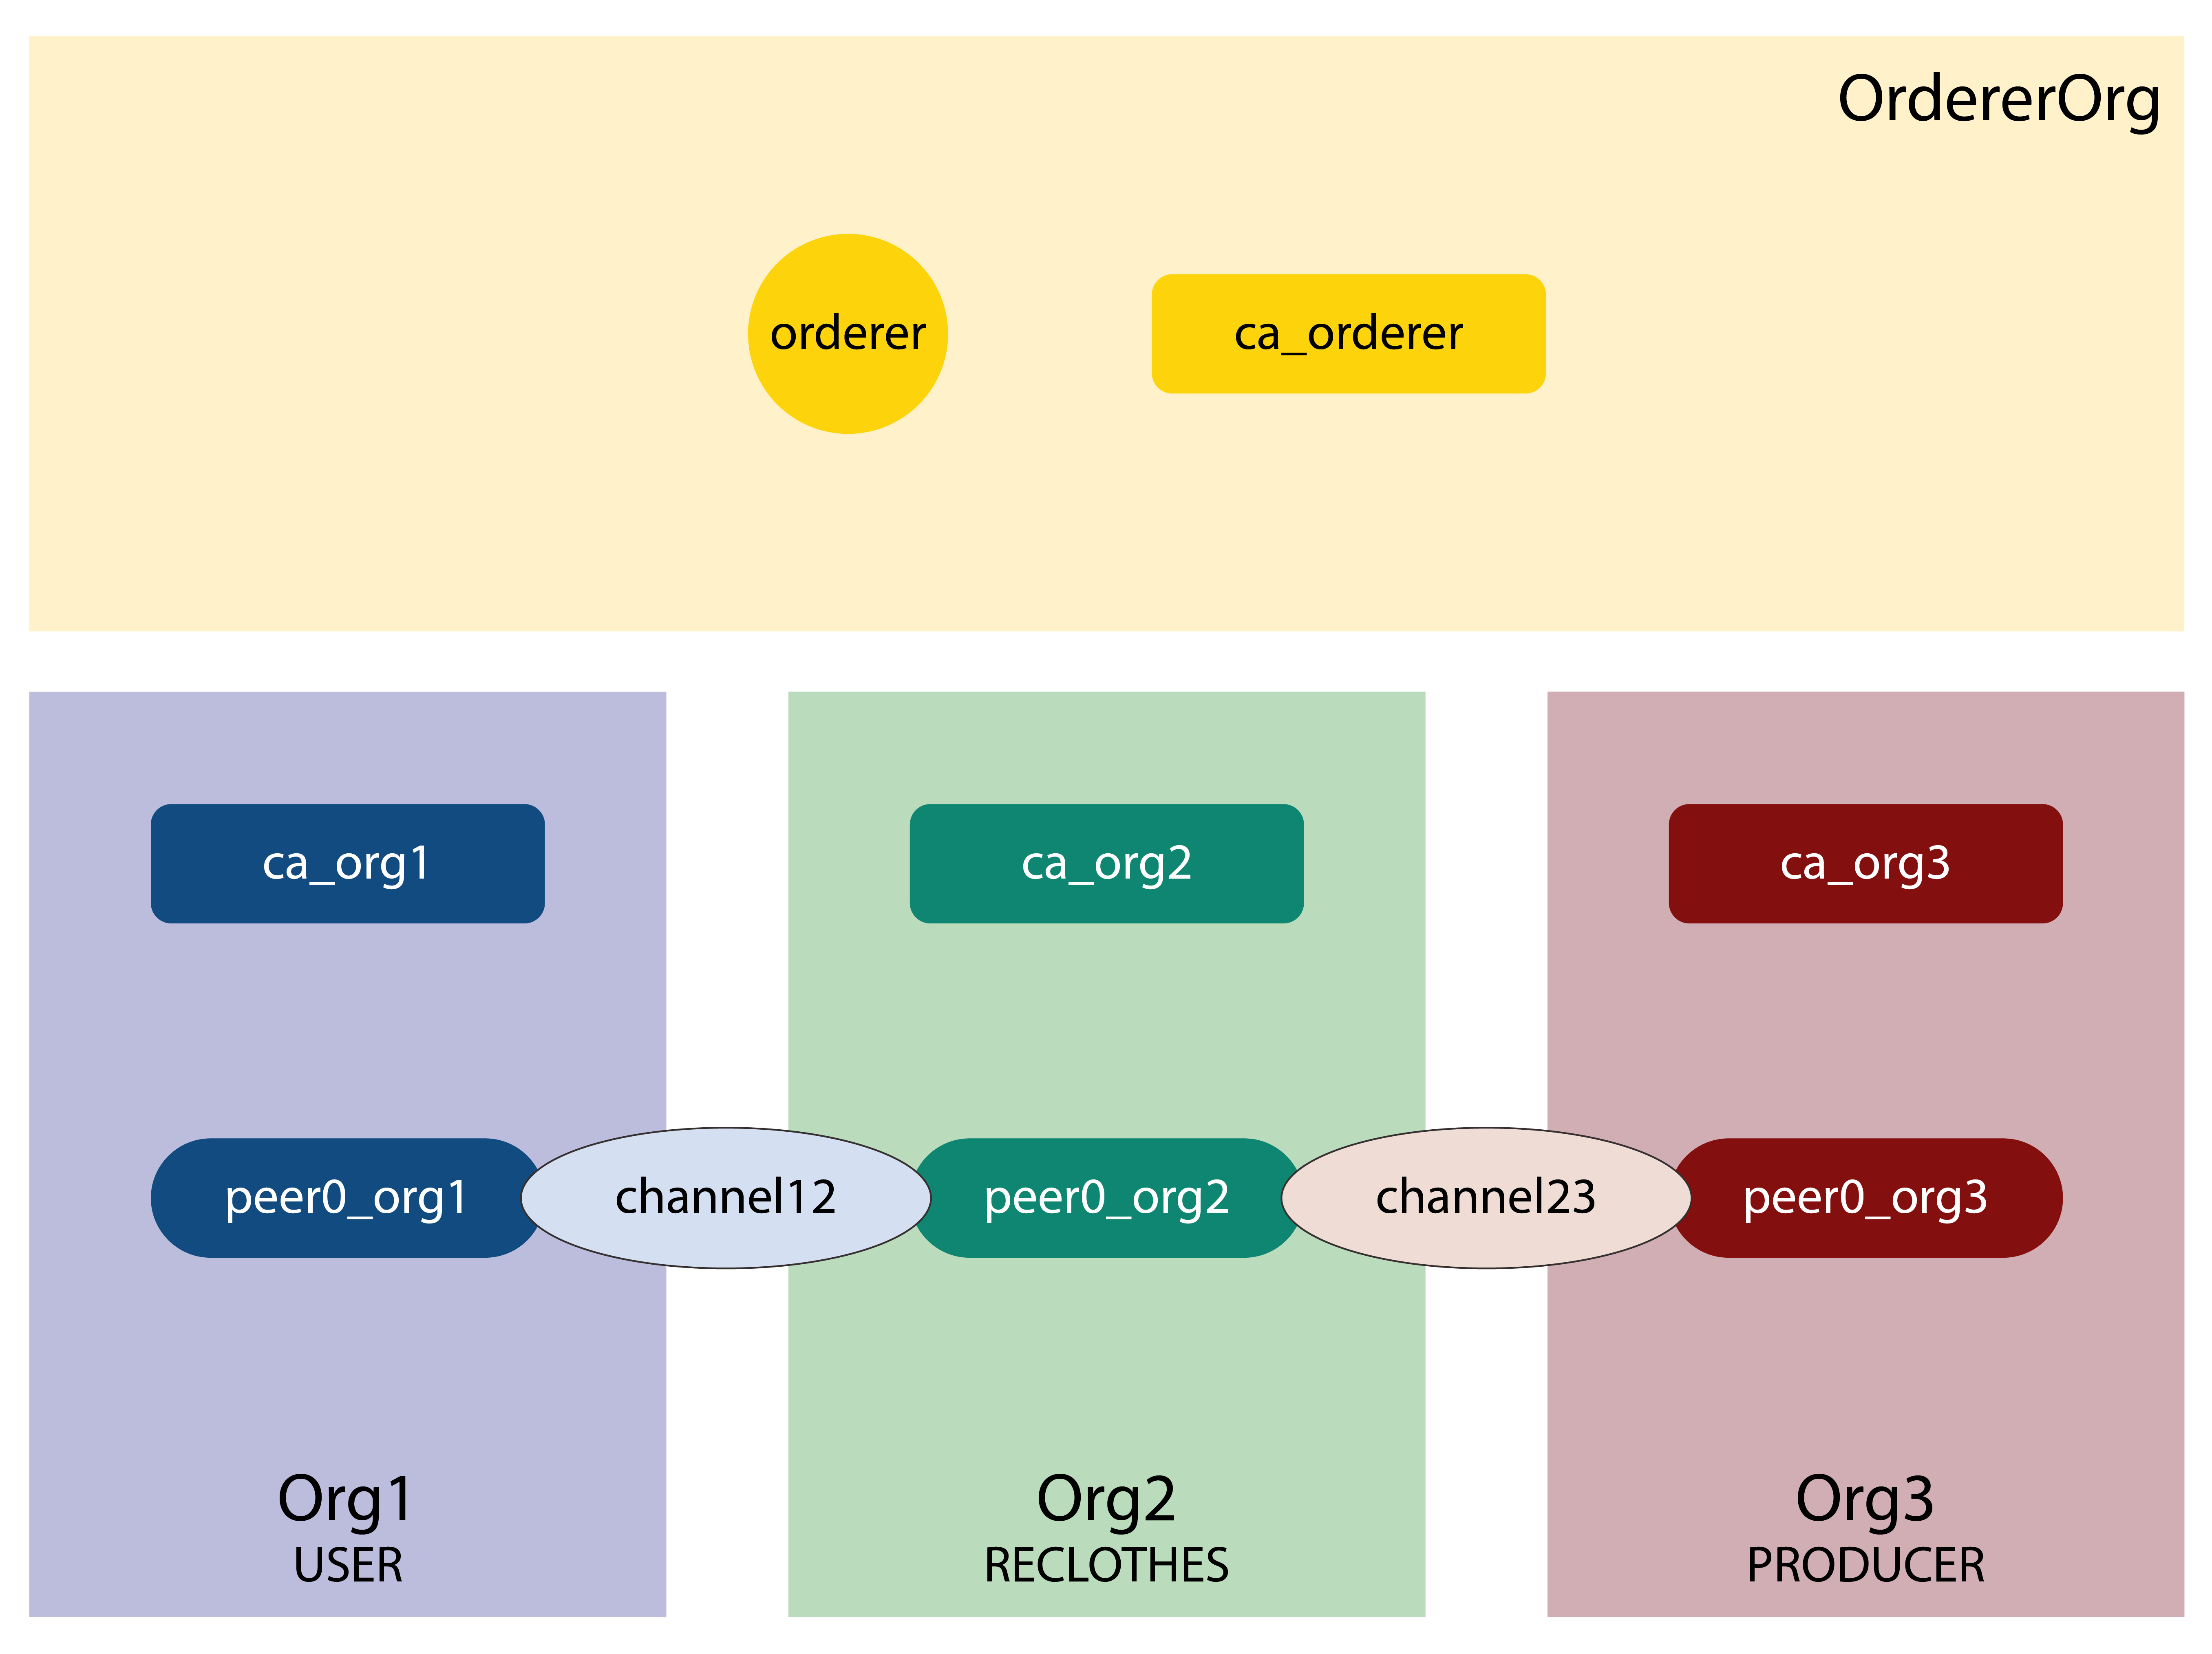
\includegraphics[totalheight=10cm]{img/fabric_network.png}
	\caption{Fabric Network}
	\label{fig:fabric_network}
\end{figure}

\subsection{Fabric Network}

\textbf{Figure \ref{fig:network}} shows how components interact each other. It is possible to separate components 
into 2 categories, inside and outside Fabric Network. First of all we need to describe the components involved:

\begin{outline}
    \1 \textbf{Web3 App}: It is the Dapp and the Client connection to the network.
    \1 \textbf{Channel}: It is the channel above which transfers data. 
    \1 \textbf{CA}: It is the Certification Authority in charge of release certificates.
    \1 \textbf{Peer}: It is "Fabric node", the endpoint of the internal network. It owns by specific CA with 
    fixed rights, linked to the connected channels. 
    \1 \textbf{evm SC}: It is the Ethereum Virtual Machine Chaicode, used to run Solidity Smart Contract. The chaincode 
    is installed over the peer.
    \1 \textbf{ledger}: It is the ledger associated to the channel connected. There is a 1 to 1 association 
    between ledger and channel.
    \1 \textbf{CC}: It is the \textit{Consortium}, It is associated to the channel, it manages ownerships and 
    it includes a set of Organizations allowed. 
    \1 \textbf{Docker}: The network components run inside docker container. 
\end{outline}

\begin{figure}[h!]
	\centering
	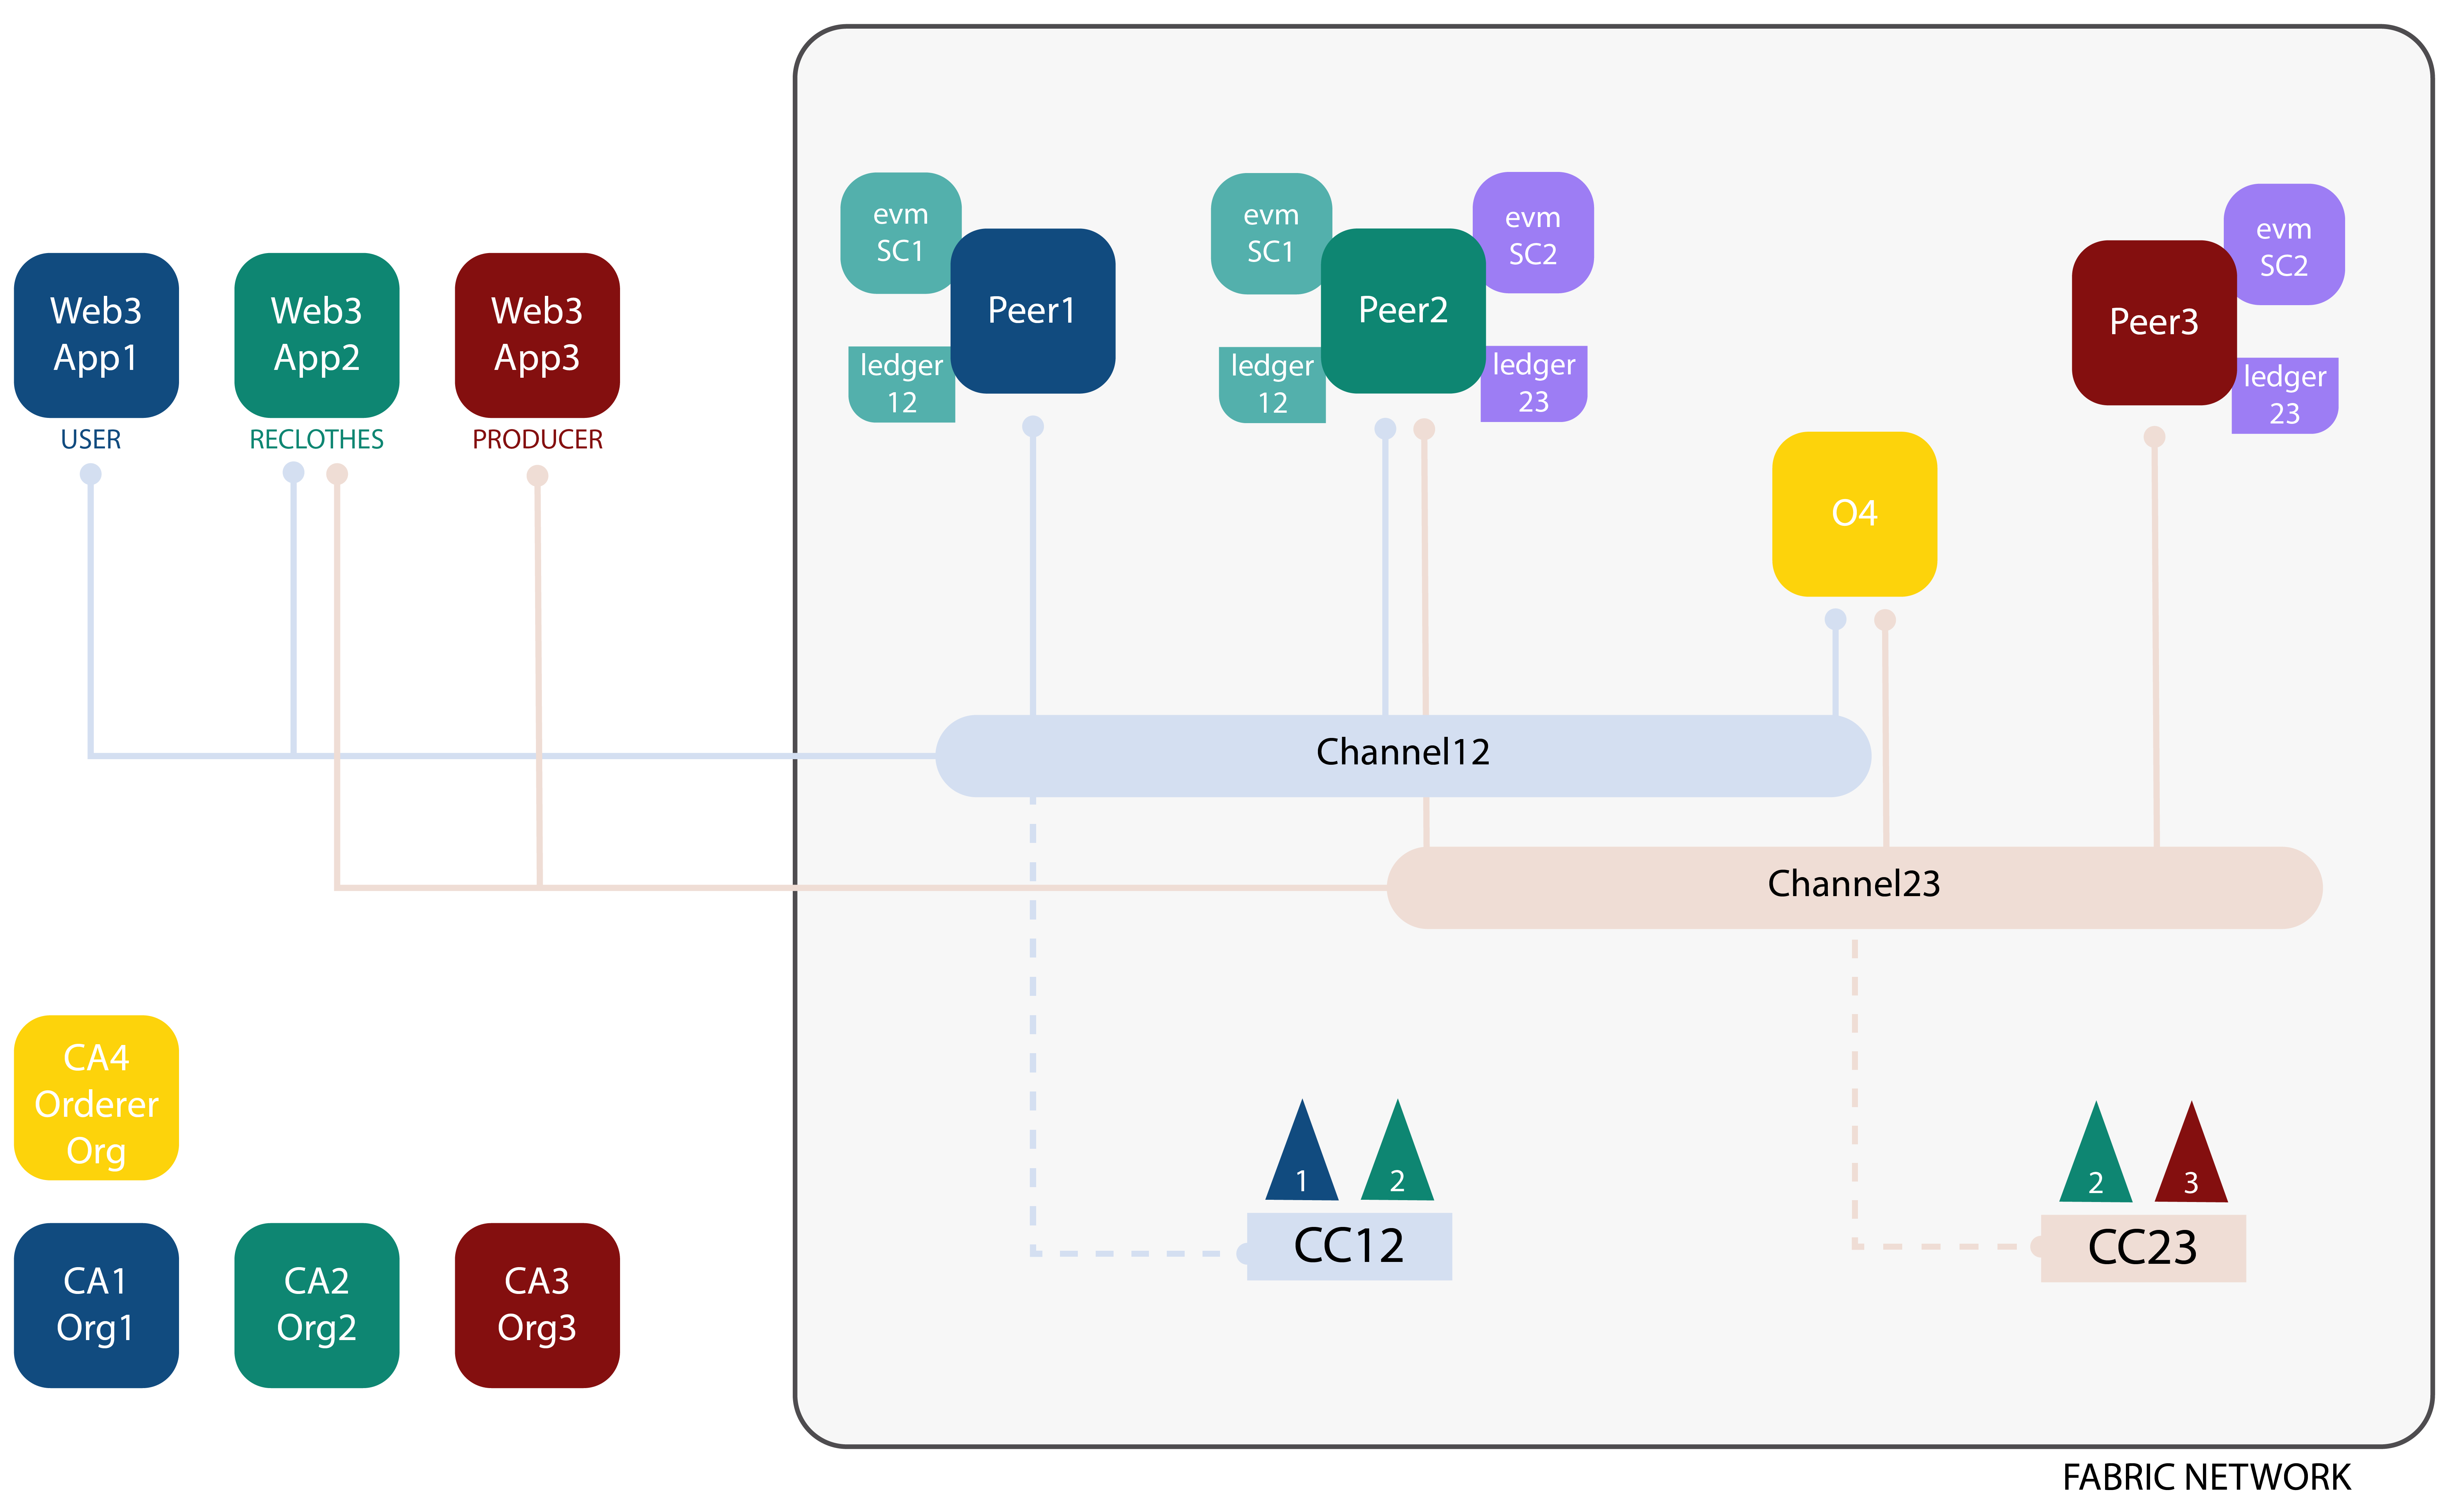
\includegraphics[totalheight=10cm]{img/network.png}
	\caption{Fabric Network Components}
	\label{fig:network}
\end{figure}

By Figure \ref{fig:network} it is possible to see that in the architecture there are two ledgers, each of that 
associated with one channel that involves just part of organizations per channel. The ledger is associated with 
one or more smart contract deployed over the chaincode, in own case we use 1 smart contract deployed each chaincode. 

The \textit{chaincode} is invoked calling the EVM chaincode by the \textit{App} Client, using channel communication.
The channel is the only communication way between outside and inside the network. The external actor that invoke the chaincode
must have the privileges to join the specified channel. 
The chaincode installed over the peer once is invoked agreed to the request and invoke the chaincode("smart contract")
method. 

Once the method returns, the chaincode forwards the reply to the App client. Then the Dapp forward the
answer to the \textit{Orderer} peer that validates the response, create a new block, add it to the chain,
communicate it to the peer in order to synchronize the network and updating the Ledger World State.

\subsubsection{Config File}

The network architecture in Hyperledger Fabric is highly modular and scalable. Hyperledger provides to the developers a set of developed 
test network\cite{fabric-sample} for testing purpose and that help developers to better understand
the structure and the steps of the creation. The \texttt{fabric-samples} contains a set of tools that allow releasing all the cryptographic
materials required for the usage of the network, such as certificates related to the user belonging to a specific organization.
In other words, all the MSP works are handled by fabric-samples tools. 
\bigskip

The most useful thing about the Hyperledger network is that the components could be added or removed in an easy way.
To design and set up network components and rules, it is has been written the \texttt{config.yaml} file.

The \texttt{config.yaml} is structured in the following way:
\begin{outline}
    \1 \textbf{Organizations}: here must be listed all the organizations involved in the network, specifying the MSP and
    the policies of each Org. 
    \1 \textbf{Consortium}: once the organizations are specified, the file defines the consortiums involved in the network.
    The consortium will be joint to specific channels. 
    \1 \textbf{Channels}: in the last section must be specified the channels of the networks, specifying the consortium
    and the related organizations allowed over the channel. 

\end{outline}

\subsubsection{Run of the network}

To set up the network in the best way, some scripts that performs the integration of several components 
in the best way, are created.

The macro process flow of the network running is:
\begin{outline}[enumerate]
    \1 \textbf{Check Prerequisite}: using the \texttt{fabric-samples}\cite{fabric-sample} there is
    some prerequisite to check, to run all the materials in the correct way. Check the prerequisite looking at fabric 
    documentations\cite{fabric-doc}.
    \1 \textbf{Run Network}: Once the \texttt{config} file is designed and developed, we need to include evm chaincode 
    in the volumes of docker files. Then it is possible to run the network.
    \1 \textbf{Join all the components}: Once the network is in running, it is important to join all the components each 
    other, for example join the peers to the dedicated channels.
    \1 \textbf{Chaincode}: Once that all components are set up in the right way and the network is in running, it is 
    possible to install the chaincode over the peers that we want to use. 
\end{outline}

The Hyperledger Fabric network runs inside \textbf{docker containers}. To automatize the running 
of the network I created scripts that setup Fabric locally using docker containers, install the EVM chaincode (EVMCC) 
and instantiate the EVMCC over the Fabric peers. All that thesis steps use the Hyperledger \texttt{fabric-sample} 
repository to deploy Fabric locally and the \texttt{fabric-chaincode-evm} repo for the EVMCC.

The scripts developed are the following ones:

\begin{outline}
    \1 \textbf{\texttt{net\_up.sh}}:
    \2 \textbf{Generate crypto materials for organizations}: First of all, using the \texttt{fabric-sample} supplied
    by IBM, it is possible to run a tool in charge of creating all the cryptographic material for the actors 
    used to operate over the network. 
    \2 \textbf{Generate channel artifacts}: In the same way, the cryptographic materials generated for the 
    Organizations must be generated for the channel involved in the network.
    \2 \textbf{Run docker containers}: Once the crypto materials are created then it must run the docker containers
    for the components of the networks. The \textbf{Figure \ref{fig:docker-run}} shows the related output.
    \2 \textbf{Initialize Orgs and join them to the channels}: Once all the containers are in running then there are
    the organization's initializations and each peer owner by an Org is joined to the channel following
    the \texttt{config file} specifications. \textbf{Figure \ref{fig:init-org}} shows the related output.
    \2 \textbf{Instantiate and Install evm chaincode}: Once all the network is in running we are going to install 
    the chaincode over the peers. In my case, we are going to install \texttt{fabric-chaincode-evm}.
    \textbf{Figure \ref{fig:install-chaincode}} shows the related output.

    \1 \textbf{\texttt{net\_down.sh}}:
    \2 \textbf{remove all docker containers in running}
    \2 \textbf{remove all docker volumes created}

    \1 \textbf{\texttt{fab1.sh}}:
    \2 \textbf{network-sdk-config.yaml}: It is the mapping SDK file from web3js request to the fabric requests. 

\end{outline}

\begin{figure}[!ht]
    \centering
    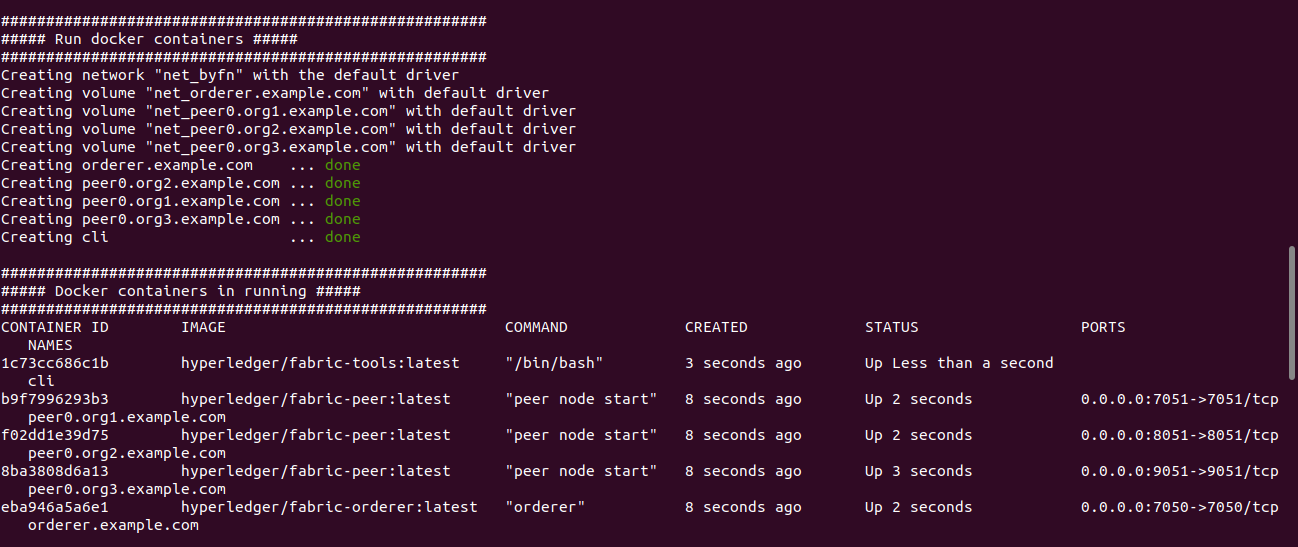
\includegraphics[totalheight=6cm]{img/network/net-1.png}
    \caption{Run of the Docker Containers}
    \label{fig:docker-run}
\end{figure}

\begin{figure}[!ht]
    \centering
    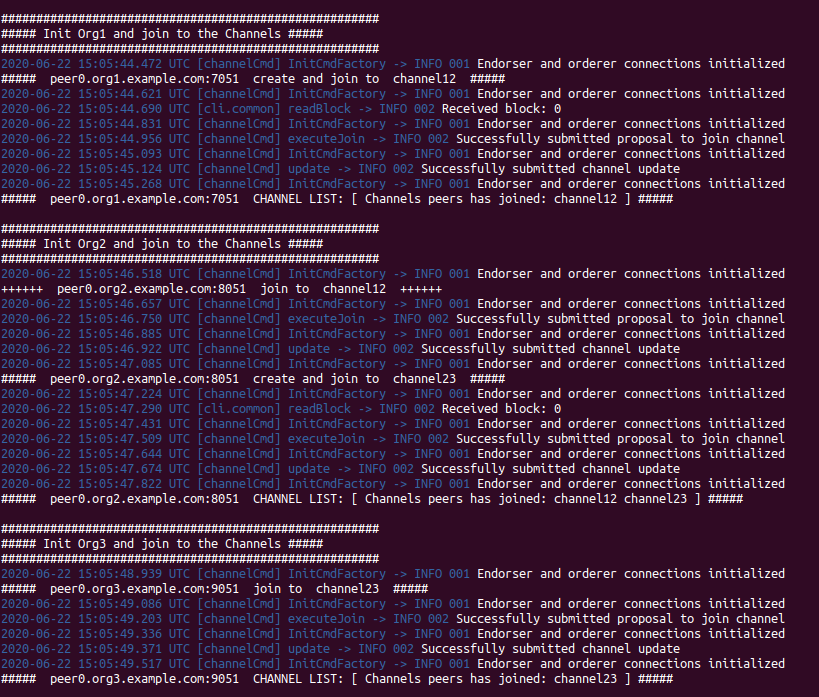
\includegraphics[totalheight=8cm]{img/network/net-2.png}
    \caption{Orgs initializations and channels join}
    \label{fig:init-org}
\end{figure}

\begin{figure}[!ht]
    \centering
    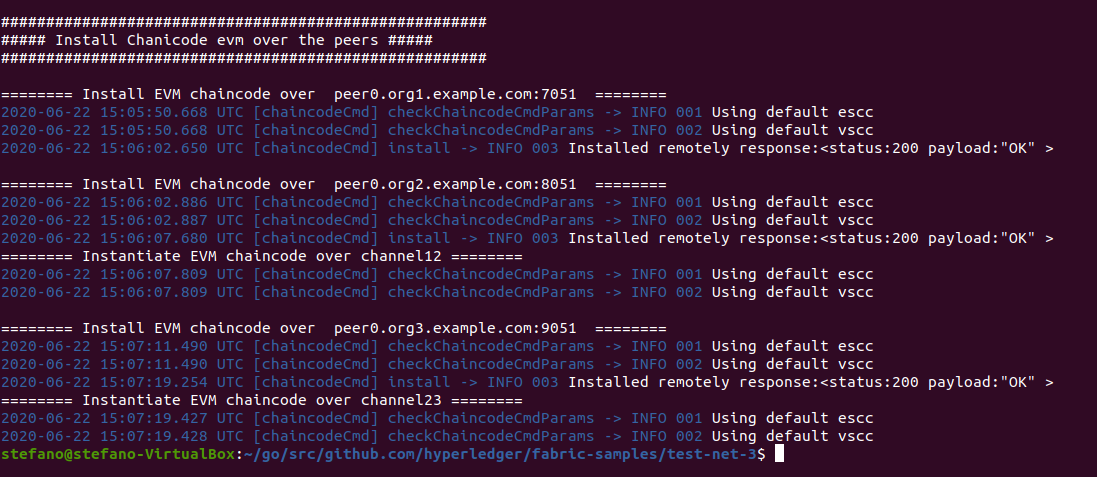
\includegraphics[totalheight=6cm]{img/network/net-3.png}
    \caption{Chaincode Installation}
    \label{fig:install-chaincode}
\end{figure}

\newpage
\subsubsection{Scripts produced}

For a better understanding of the setting up and running of the entire network, I reported below the two main scripts. 
The two files \textbf{\texttt{net\_up.sh}} and \textbf{\texttt{net\_down.sh}} show in the best way all the steps that 
allow the network running.

\textbf{\texttt{net\_up.sh}}:

\begin{lstlisting}[language=bash]
    #!/bin/bash

    ##### Generate Crypto Material for Organizations #####
    ../bin/cryptogen generate --config=./crypto-config.yaml

    ##### Build Channel Artifact #####
    ./channel_artifact.sh

    ##### Run docker containers #####
    docker-compose up -d

    ##### Docker containers in running #####
    docker ps

    ##### Init Org1 and join to the Channels #####
    docker exec cli scripts/org1_init.sh

    ##### Init Org2 and join to the Channels #####
    docker exec cli scripts/org2_init.sh

    ##### Init Org3 and join to the Channels #####
    docker exec cli scripts/org3_init.sh

    ##### Install Chanicode evm over the peers #####
    docker exec cli scripts/install.sh
\end{lstlisting}

\bigskip

\textbf{\texttt{net\_down.sh}}:

\begin{lstlisting}[language=bash]
    #!/bin/bash

    # STOP AND DELETE THE DOCKER CONTAINERS
    docker-compose down -v
    docker rm $(docker ps -aq)
    docker rmi $(docker images dev-* -q)

    # DELETE THE OLD DOCKER VOLUMES
    docker volume prune

    # DELETE OLD DOCKER NETWORKS (OPTIONAL: seems to restart fine without)
    docker-compose -f  down --volumes --remove-orphans
    docker network prune

    # DELETE SCRIPT-CREATED FILES
    rm -rf channel-artifacts/*.block channel-artifacts/*.tx crypto-config

    # Remove created folder
    rm -rf channel-artifacts

    # VERIFY RESULTS
    docker ps -a
    docker volume ls
    ls -l
\end{lstlisting}

\subsection{Ethereum Network - Ropsten}

To run the ERC20 token it is used the testnet Ropsten against the mainnet. 
To set up and upload the ERC20 Token over the Ethereum network it is used the following tools:

\begin{outline}
    \1 \textbf{My Ether Wallet}: To upload ERC20 contract.
    \1 \textbf{Etherscan.io}: To monitor and analyze transactions over the network.
    \1 \textbf{Metamask}: To create user wallets and sign eth transactions.
    \1 \textbf{Infura}: To set up a node in order to use it as endpoint and communicate with the Ropsten network,
    it is used as \textit{Provider} in \textit{Web3} library.  
\end{outline}

\section{Fabric and EVM chaincode interaction}

\subsection{Chaincode invocation}

To analyze how evm chaincode allows running Solidity bytecode inside Hyperledger Fabric network, first of all, we 
analyze the interaction process and chaincode invocation Process of Hyperledger Fabric blockchain. 

\subsubsection{End to End Interactions} 
Going deeper, the \textbf{Figure \ref{fig:end_to_end}} shows the flow of the end to end communication. How all the 
components are boxed inside the Peer component. The Fab3 maps the web3 request and forwards it to fabric peer. the request 
arrives at the evmcc that invokes Solidity smart contract methods.

\begin{figure}[h!]
    \centering
    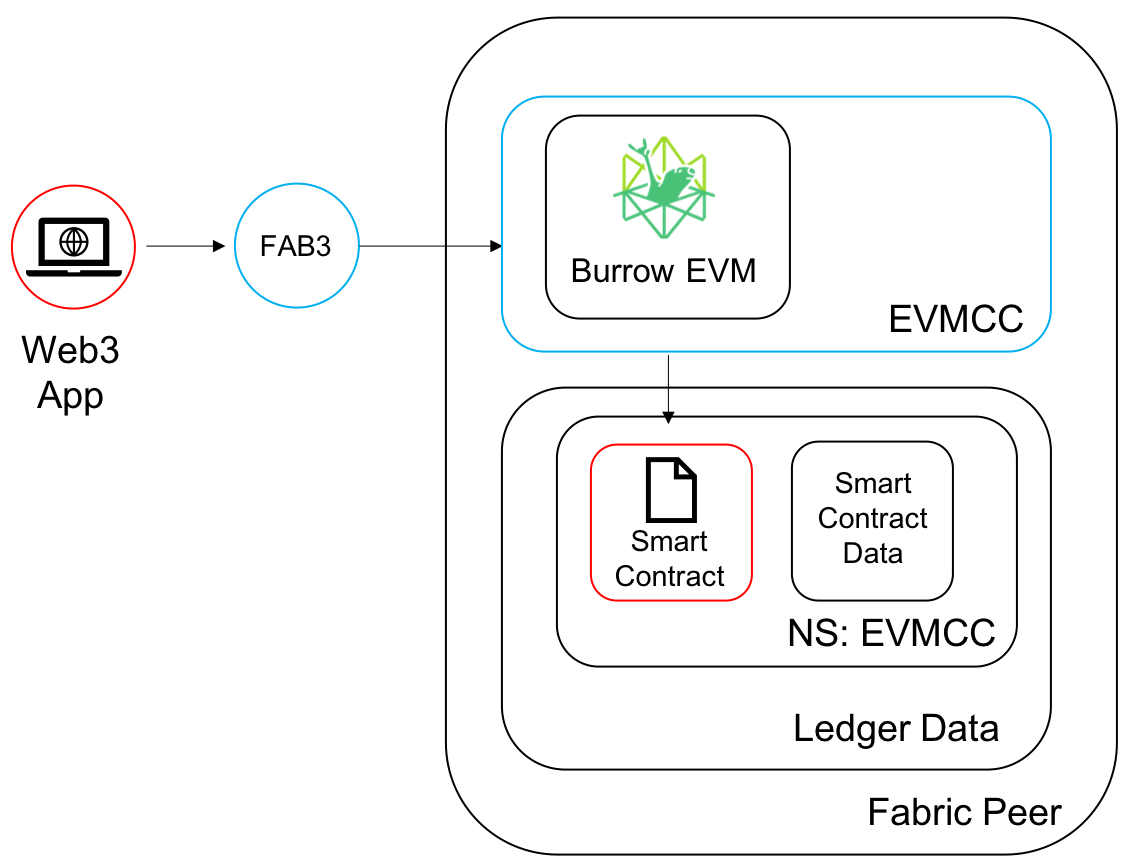
\includegraphics[totalheight=7.5cm]{img/EndToEnd.png}
    \caption{End To End}
    \label{fig:end_to_end}
\end{figure}

\subsubsection{Chaincode Invocations}
The \textbf{Figure \ref{fig:sc_invokation}} below describes the internal workflow of the chaincode invocation, where is 
involved the \textit{Client}, the \textit{Peer} and the \textit{Orderer}. All the information are transferred over the 
set channel and in the thesis work, the client doesn't interact directly but using \textit{Fab3 Proxy}
as intermediary.

\begin{figure}[h!]
    \centering
    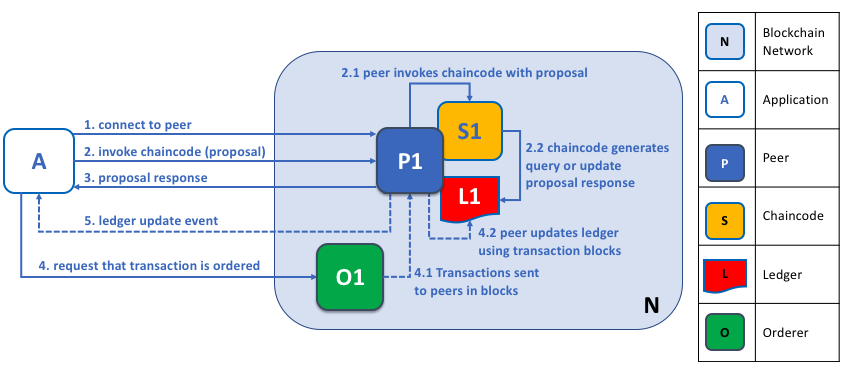
\includegraphics[totalheight=6cm]{img/sc_invokation.png}
    \caption{Smart Contract Invocation Process. Source: \url{https://hyperledger-fabric.readthedocs.io/en/release-1.4/peers/peers.html}}
    \label{fig:sc_invokation}
\end{figure}

\newpage
\subsection{Fab3 Proxy}

The Fab3 Proxy is a main component of the entire architecture. It works as a bridge between the Ethereum
world and the Hyperledger Fabric one. Each instance of Fab3 map 1 Fabric user and generates a semi-random 
Eth address starting from the public key of the user's x.509 certificate related to the Fabric identity. 
The Following environment variable set the mandatory data to run a Fab3 proxy instance:

\begin{outline}
    \1 \textbf{CONFIG}: It is the path to a compatible Fabric SDK Go config file, used to communicate and map the 
    requests and forward it to the Fabric network.
    \1 \textbf{USER}: User identity being used for the proxy. Matches the user's names in the crypto-config directory 
    specified in the config.
    \1 \textbf{ORG}: Organization of the specified user.
    \1 \textbf{CHANNEL}: Channel to be used for the transactions.
    \1 \textbf{CCID}: ID of the EVM chaincode deployed in your fabric network.
    \1 \textbf{PORT}: Port the proxy will listen on. If not provided default is 5000
\end{outline}

Below there is an example of environments variable setting up used to run Fab3 instance.

\begin{lstlisting}
# Environment variables required for setting up Fab3
export FAB3_CONFIG=${GOPATH}/src/github.com/hyperledger/fabric-chaincode-evm/examples/network-sdk-config.yaml 
export FAB3_USER=User1 
export FAB3_ORG=Org1
export FAB3_CHANNEL=channel12 
export FAB3_CCID=evmcc
export FAB3_PORT=5000
\end{lstlisting}

Once the Fab3 is set up and the instance is in running it is allowed to perform chaincode invocation using the 
thesis's Dapp. \textbf{Figure \ref{fig:fab3_flow}} shows the flow of the invocation process at upper level. 
It shows the main components that are involved in that process. 

\begin{outline}[enumerate]
    \1 \textbf{Dapp} calls method that performs smart contract invocation.
    \1 \textbf{Fab3} maps the request and forwards it to Fabric network.
    \1 \textbf{Fabric network} processes the request and issues a response.
\end{outline}

\begin{figure}[h!]
    \centering
    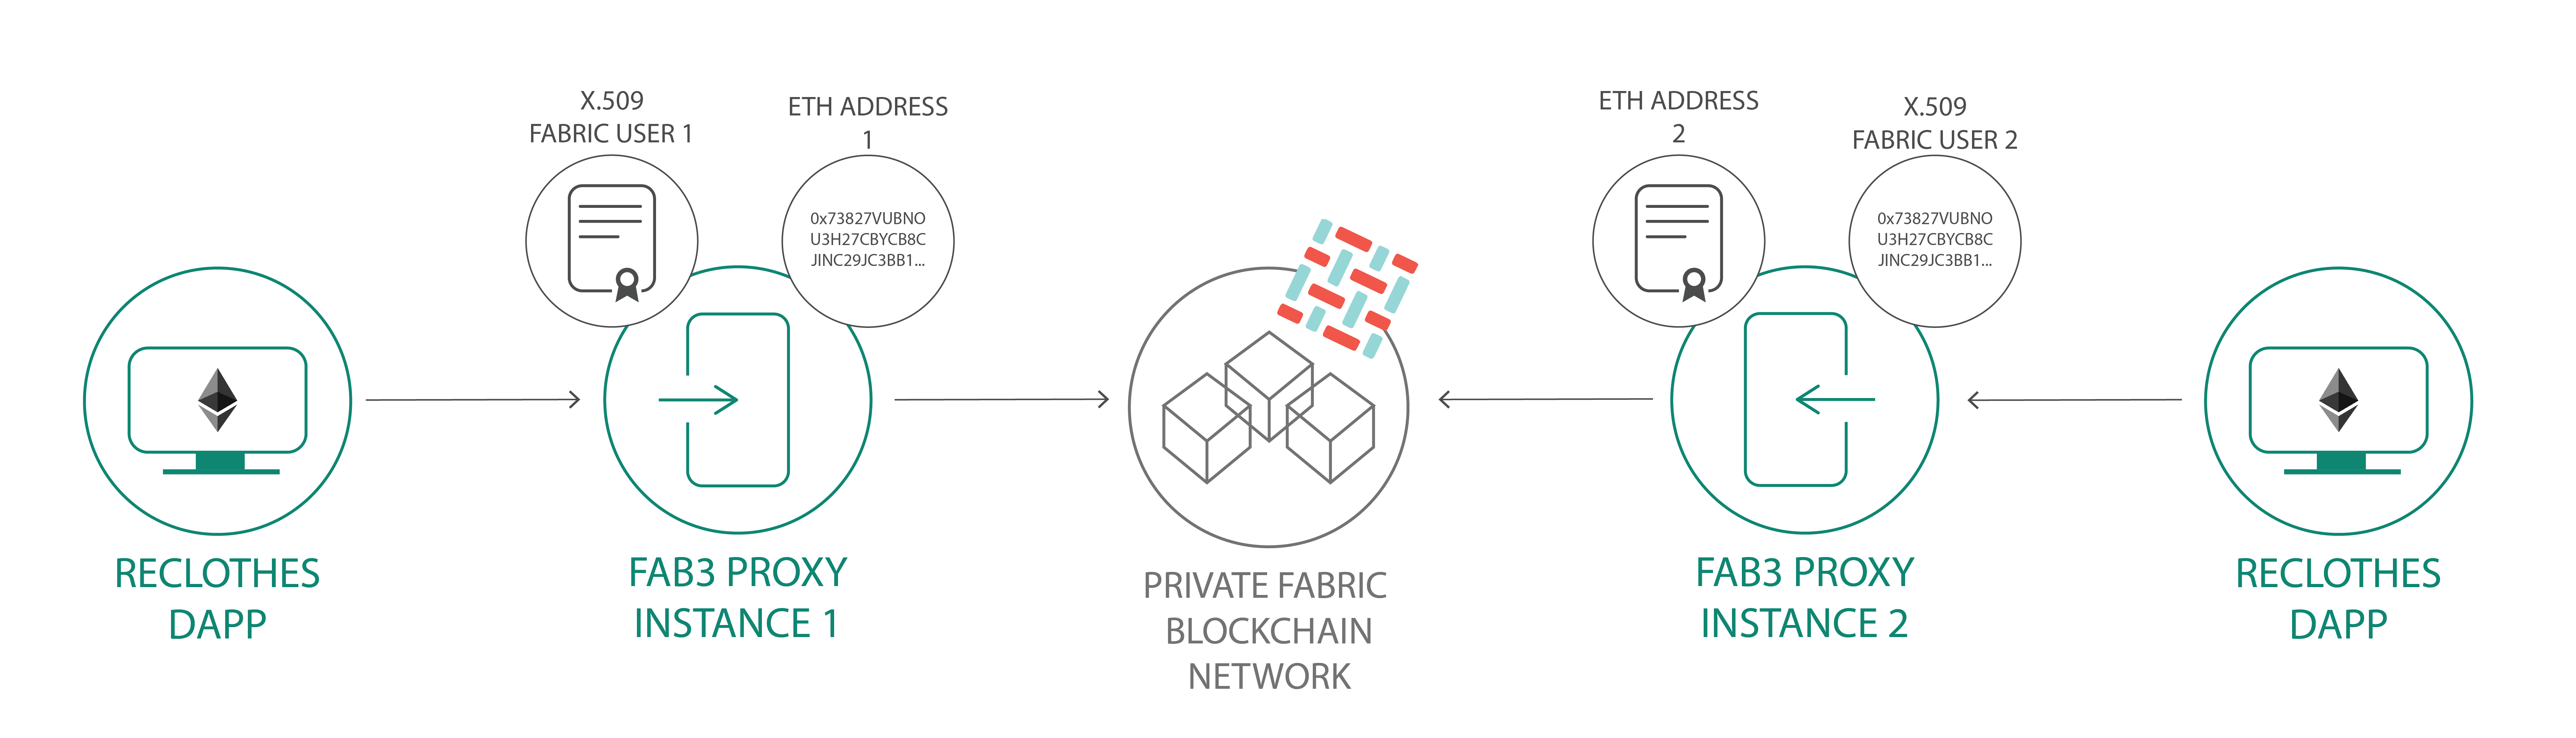
\includegraphics[totalheight=5cm]{img/fab3_flow.png}
    \caption{Fab3 Proxy Flow}
    \label{fig:fab3_flow}
\end{figure}

The \textbf{Figure \ref{fig:fab3_invokation}} shows the internal components that take part to the invocation process. 
Fab3 agreed to the request using \textit{Ethereum JSON RPC API}, map it and forward it to the Fabric network using 
\textit{GO SDK}. Once the request arrives at \textit{EVMCC}, it invokes smart contract bytecode and then follows the 
standard process explained in Figure \ref{fig:sc_invokation}.

\begin{figure}[h!]
    \centering
    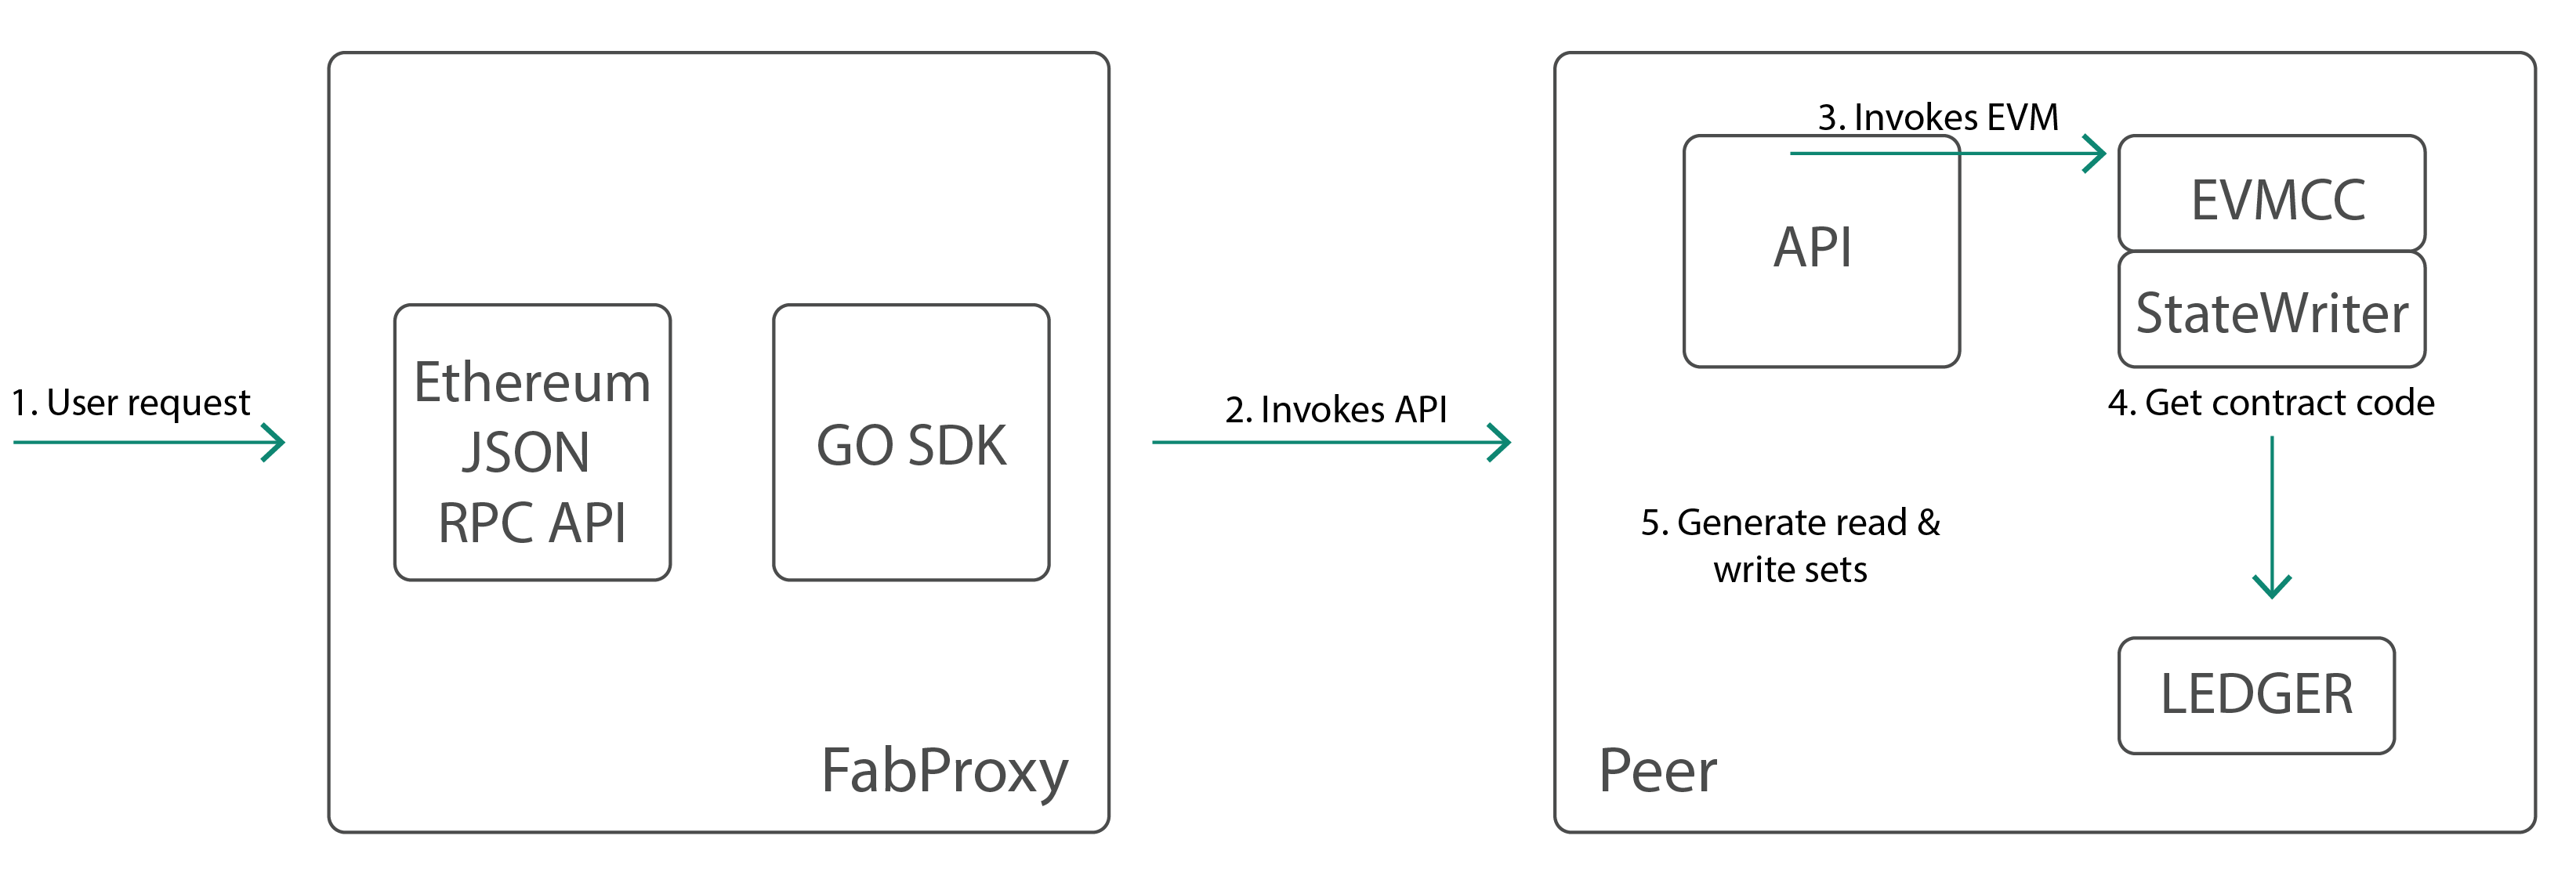
\includegraphics[totalheight=5cm]{img/fab3_invokation.png}
    \caption{Fab3 Invocation Process}
    \label{fig:fab3_invokation}
\end{figure}


% DAPP
\newpage
\section{Dapp}

\subsection{Technologies used}

The client application is a web app, composed by a front-end part and a mid-level with API that allows
the communication with smart contracts of both Blockchains. The technologies used are the following one:

\begin{outline}
    \1 \textbf{Expressjs}: It is a node.js framework that allows developing API for the application.
    \1 \textbf{Bootstrap}: To build a user-friendly front-end in order to interact in the best way.
    \1 \textbf{Web3}: Ethereum Javascript API, It is a collection of libraries that allow you to interact with a 
    local or remote Ethereum node. 
    \2 \textbf{web3 0.20.2}: used for dapp developments, Fabric side, It is a stable version and it is the version
    used in \texttt{fabric-chaincode-evm} development.
    \2 \textbf{web3 1.0.0}: used for Ethereum transactions, It is a version with more features.
\end{outline}

Starting from the Homepage the User is allowed to register itself as \textbf{User}, \textbf{Reclothes Admin}
or \textbf{Producer}.

\subsection{Core part of the web-app}

Figure \ref{fig:directory-tree} the directory tree of the web app folder. 

\begin{figure}[h!]
    \centering
    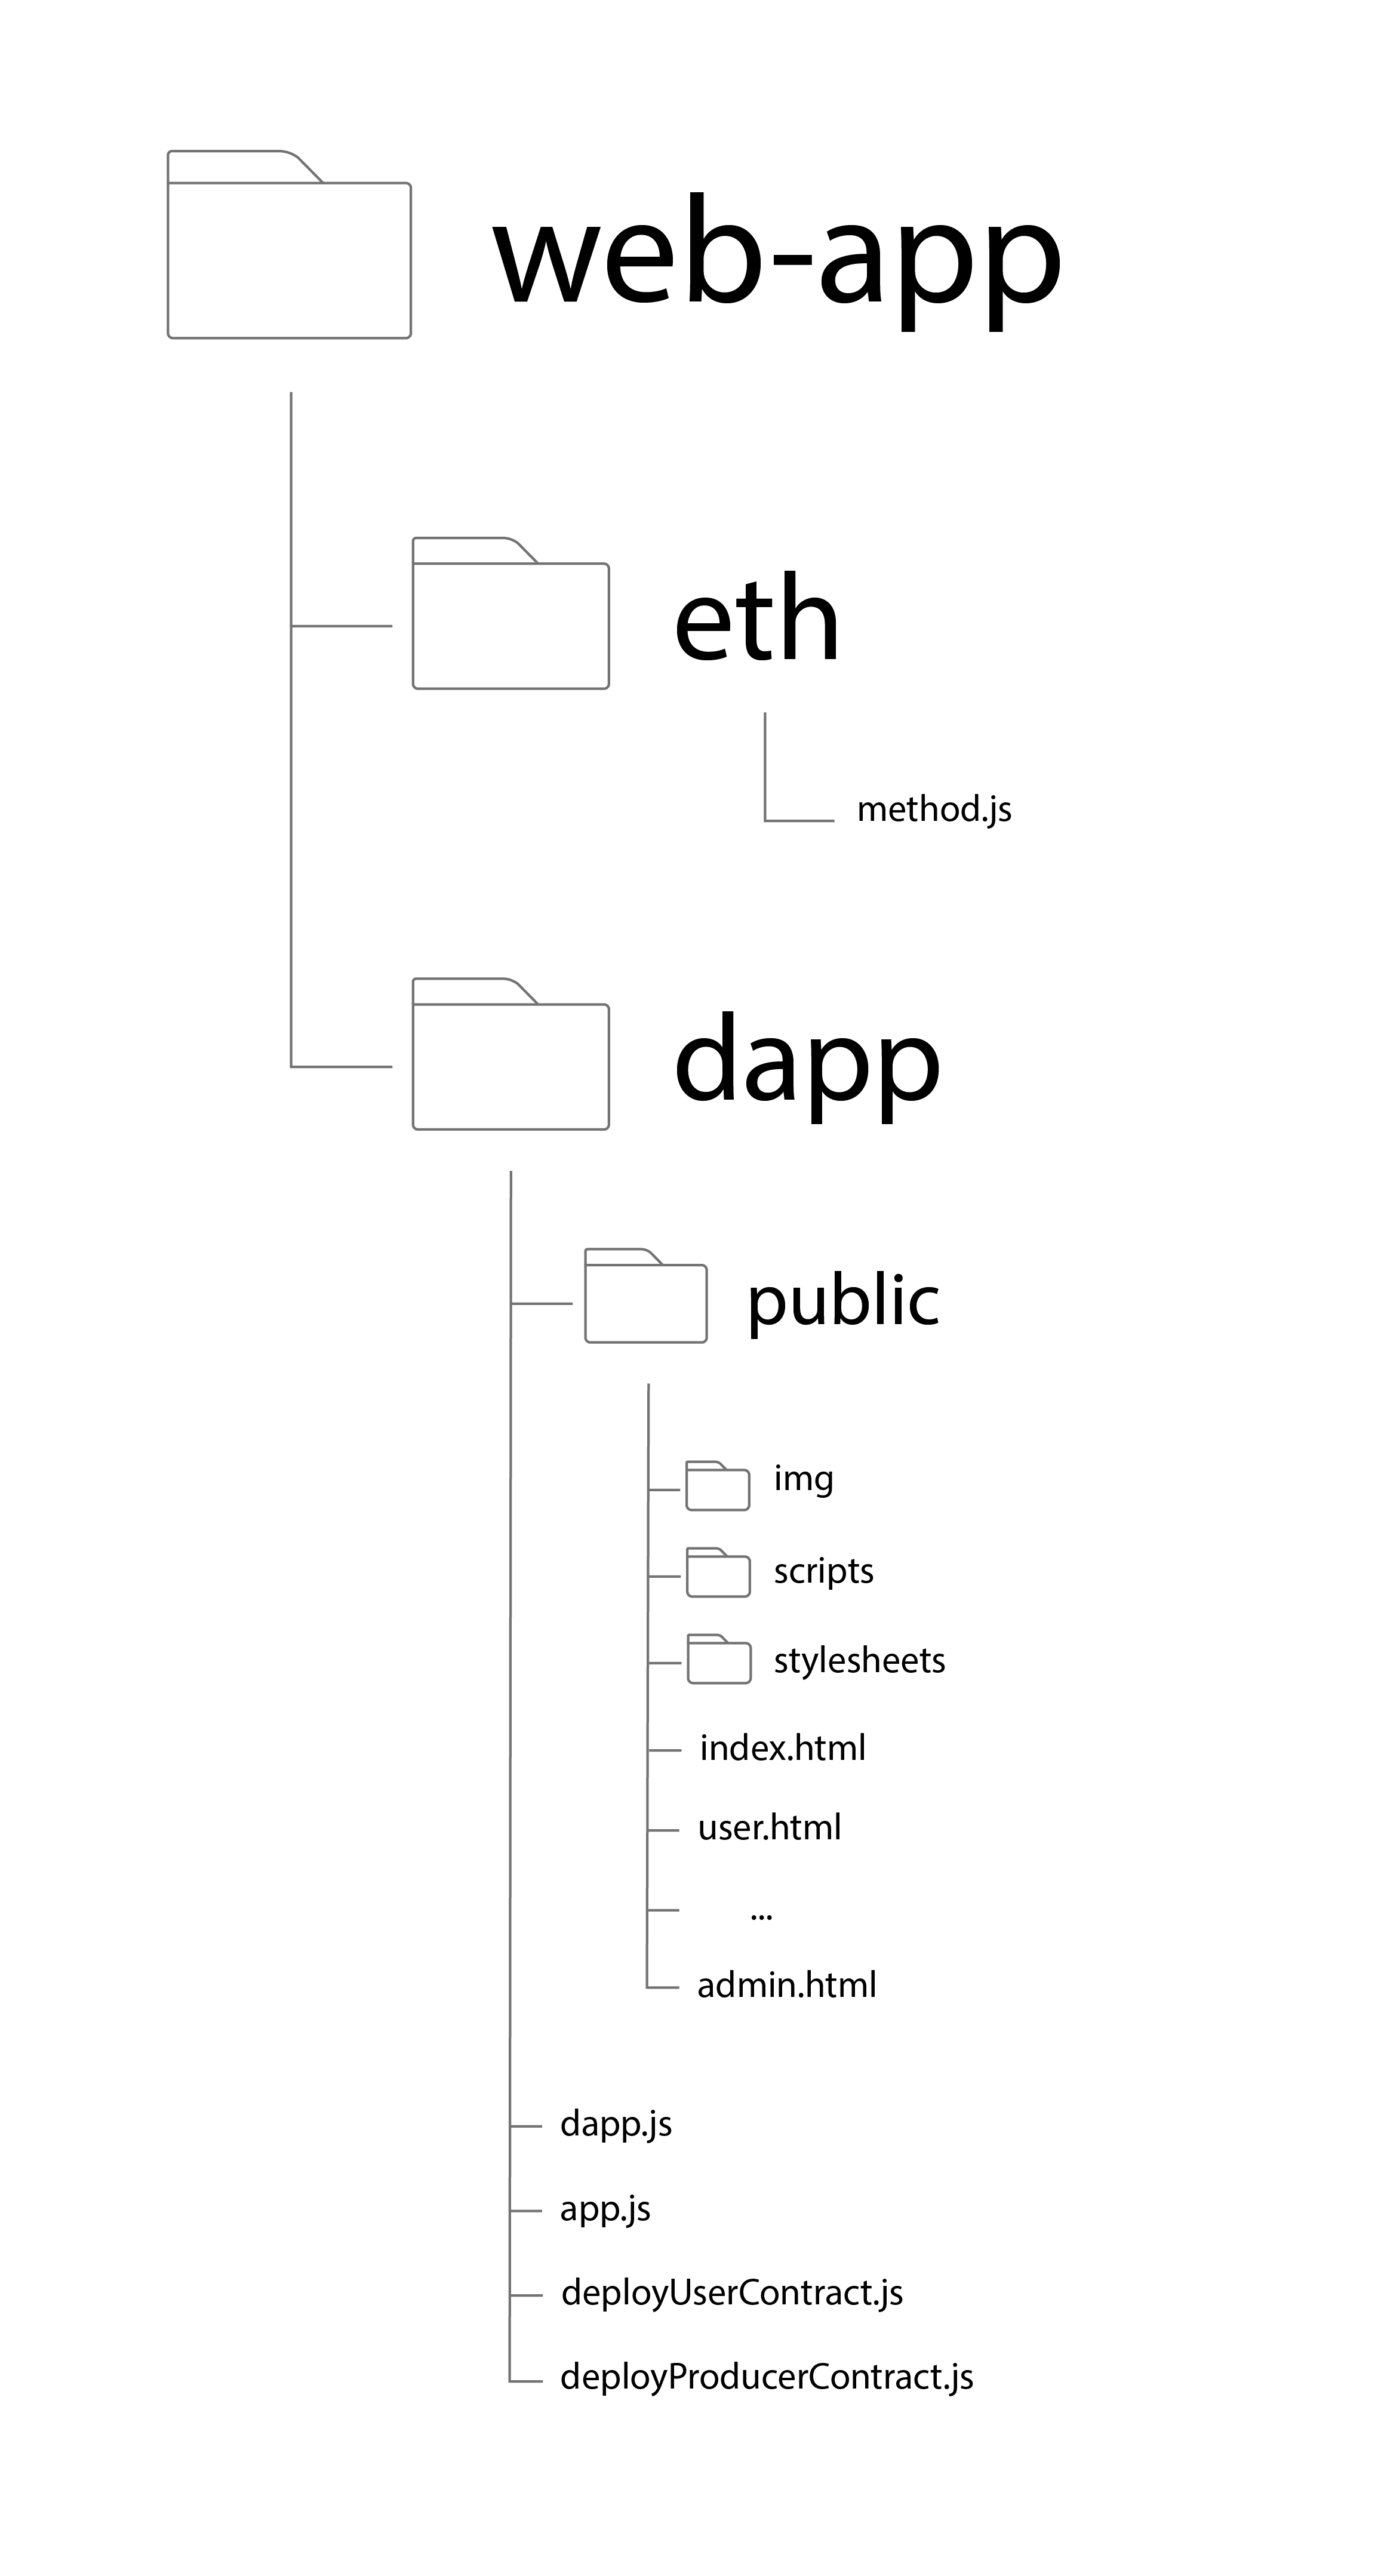
\includegraphics[totalheight=8cm]{img/directory_tree.png}
    \caption{DApp directory tree}
    \label{fig:directory-tree}
\end{figure}

The technical files and flow that dapp follows to run up it is the following one.

\begin{outline}[enumerate]
    \1 \textbf{Contract Address Generation}:
    \2 This step is in charge to run a script that deploys the contract addresses to be refereed during the 
    app running.
    \3 \textbf{deployUserContract.js}: running the script using \texttt{node .js file}, it returns the address of the 
    deployed contract. \textbf{Figure \ref{fig:deploy-user-contract}} shows the related output and the Contract 
    Address printed. 
    \3 \textbf{deployProducerContract.js}: running the script using \texttt{node .js file}, it returns the address of 
    the deployed contract. The deployed process and output is similar to Figure \ref{fig:deploy-user-contract}.
    \1  \textbf{dapp.js}: It is the core file that handles the contracts invocations, it set up the contract address 
    reference, and connect to a specific Fab3 instance.
    \1 \textbf{app.js}: It set up the API called by the web-app, it maps the request and forwards to \texttt{dapp.js}.
    \1 \textbf{method.js}: here there are all the Ethereum API endpoints. It is called by the web-app to perform 
    calls over Ethereum network. 
\end{outline}

\begin{figure}[h!]
    \centering
    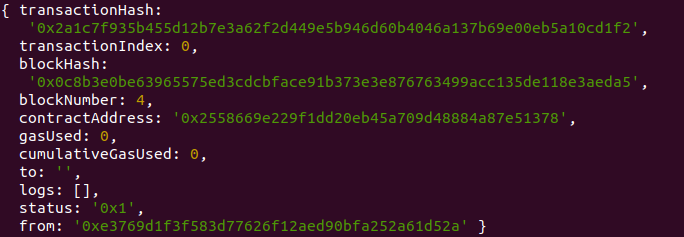
\includegraphics[totalheight=4cm]{img/app-running/deployUserContract.png}
    \caption{Deploy User Contract}
    \label{fig:deploy-user-contract}
\end{figure}

Once everything is set up, it is possible to run the web-app with the command \texttt{npm start} and there is an initialization
phase. After that, the app is ready to be used and in running over the specified PORT. The \textbf{Figure \ref{fig:app-running}}
shows the output. 

\begin{figure}[h!]
    \centering
    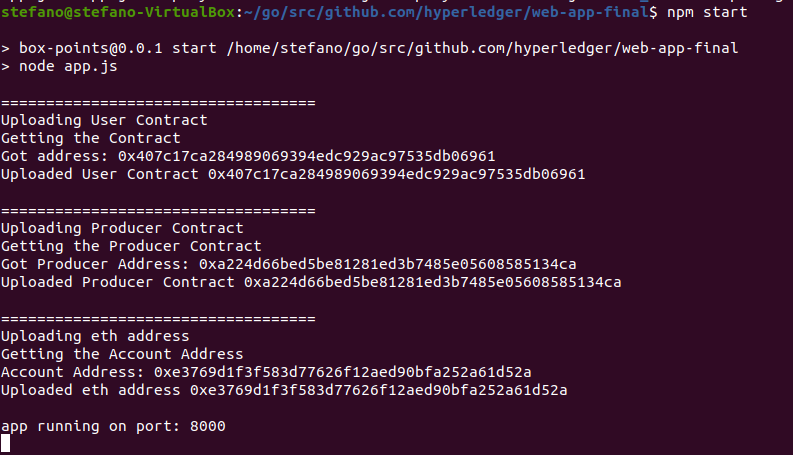
\includegraphics[totalheight=6cm]{img/app-running/app-running.png}
    \caption{App Running}
    \label{fig:app-running}
\end{figure}

\newpage
\subsection{Views}

Below I list all the views produced in the thesis work. For a better usability and understand of application behaviors,
I care about the UI too. 

\subsubsection{Homepage}

The homepage allows user to view the feature of each User type and to access to the registration page.

\begin{figure}[h!]
    \centering
    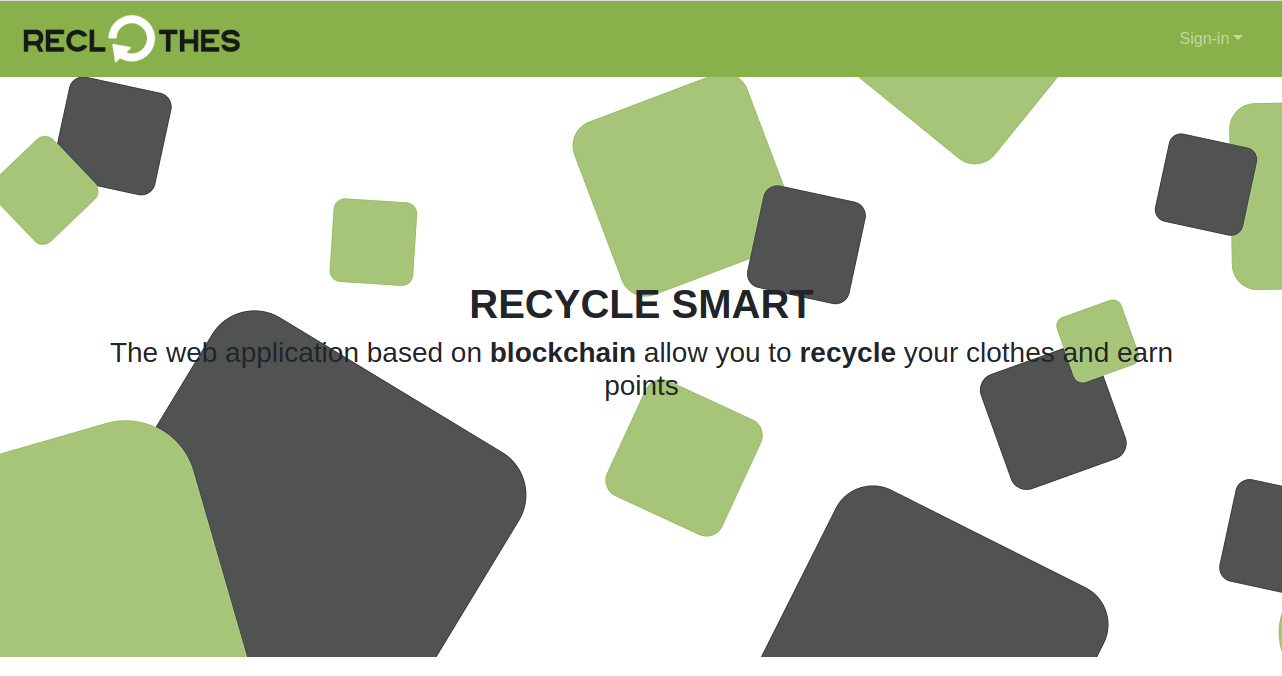
\includegraphics[totalheight=7.5cm]{img/dapp/home1.png}
    \caption{Home}
    \label{fig:home}
\end{figure}

\begin{figure}[h!]
    \centering
    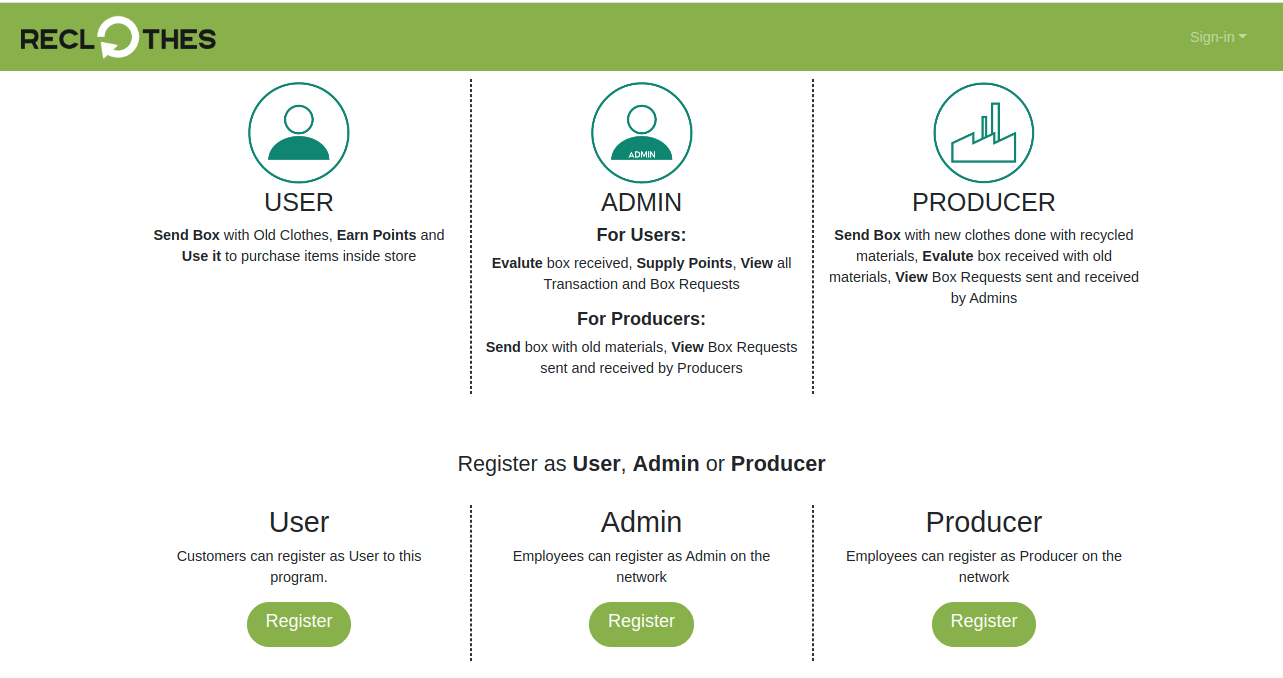
\includegraphics[totalheight=7.5cm]{img/dapp/home2.png}
    \caption{Registration Phase}
    \label{fig:registration}
\end{figure}

\newpage
\subsubsection{User Page}

The User page allows to view an overview infos once the user is logged in. 

\begin{enumerate}[-]
    \item \textbf{Address}: It is the public eth address setup during registration phase. 
    \item \textbf{Points Balance}: It is the Fabric points balance earned by the user sending the boxes.
    \item \textbf{ERC20 Balance}: It is the eth balance of the public token running over eth network.
\end{enumerate}

\textbf{Figure \ref{fig:send_box}} shows how to compile the form in order to send box with old clothes. 
It is a simulation of the real process of sending boxes, in the real case should be implemented using a QRCode 
or RFID placed over the boxes.

\textbf{Figure \ref{fig:purchase_clothes}} shows how the store should be. The purchasing of the items over 
the platform starts the transaction process. 

There is another section about info that the user is allowed to see. \textbf{Transactions} performed over the 
Fabric network and \textbf{Box Requests}, there is all the history about the box sent and received with all 
the related information's data.  
\clearpage

\begin{figure}[h!]
    \centering
    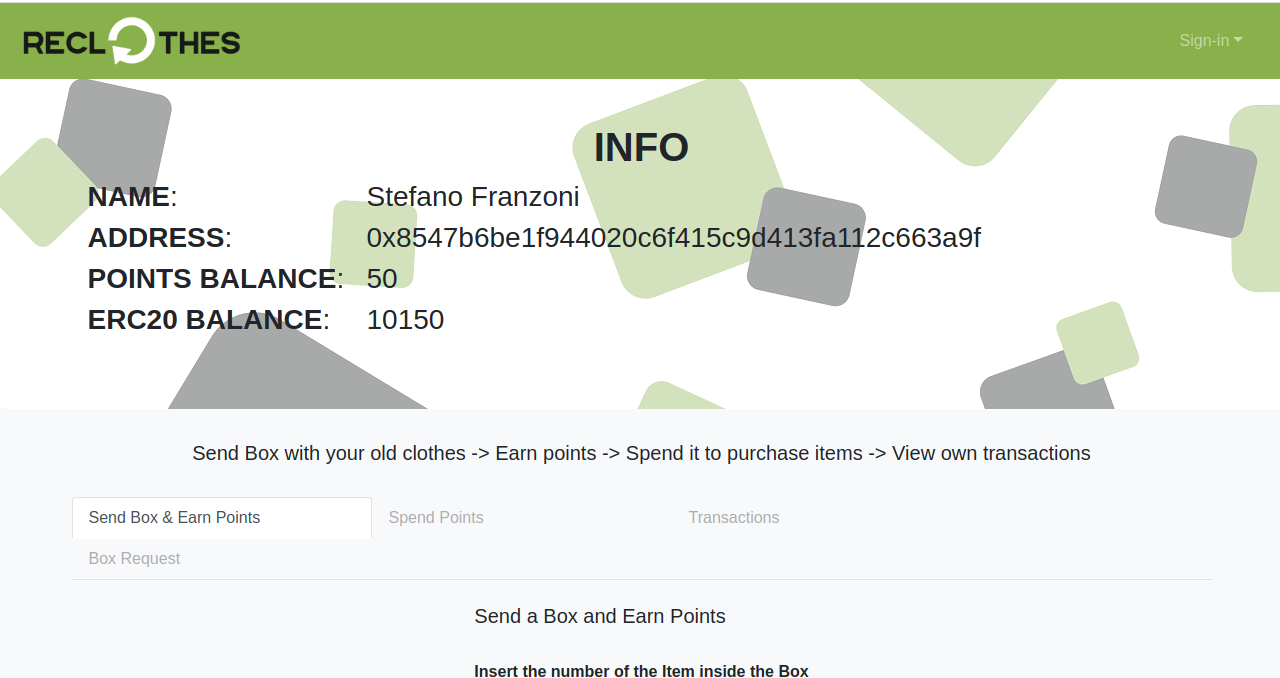
\includegraphics[totalheight=7.5cm]{img/dapp/user-info.png}
    \caption{User Info}
    \label{fig:user_info}
\end{figure}

\begin{figure}[h!]
    \centering
    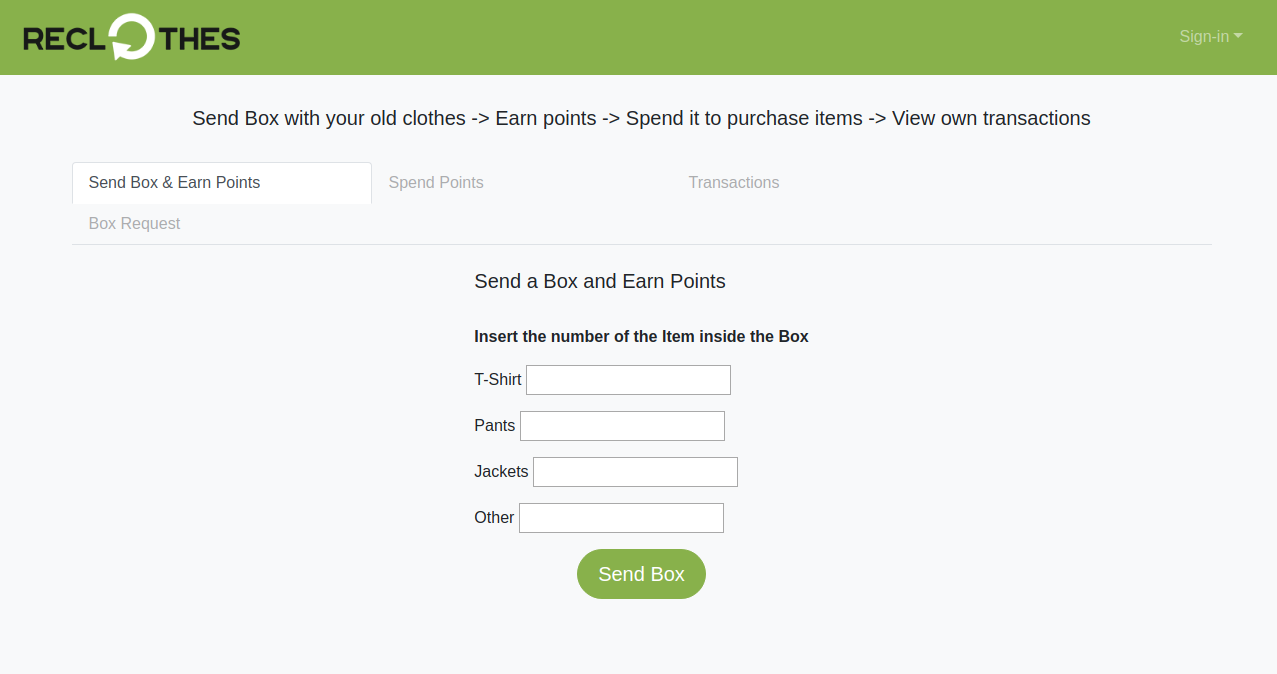
\includegraphics[totalheight=7.5cm]{img/dapp/user-send.png}
    \caption{Send Box}
    \label{fig:send_box}
\end{figure}

\begin{figure}[h!]
    \centering
    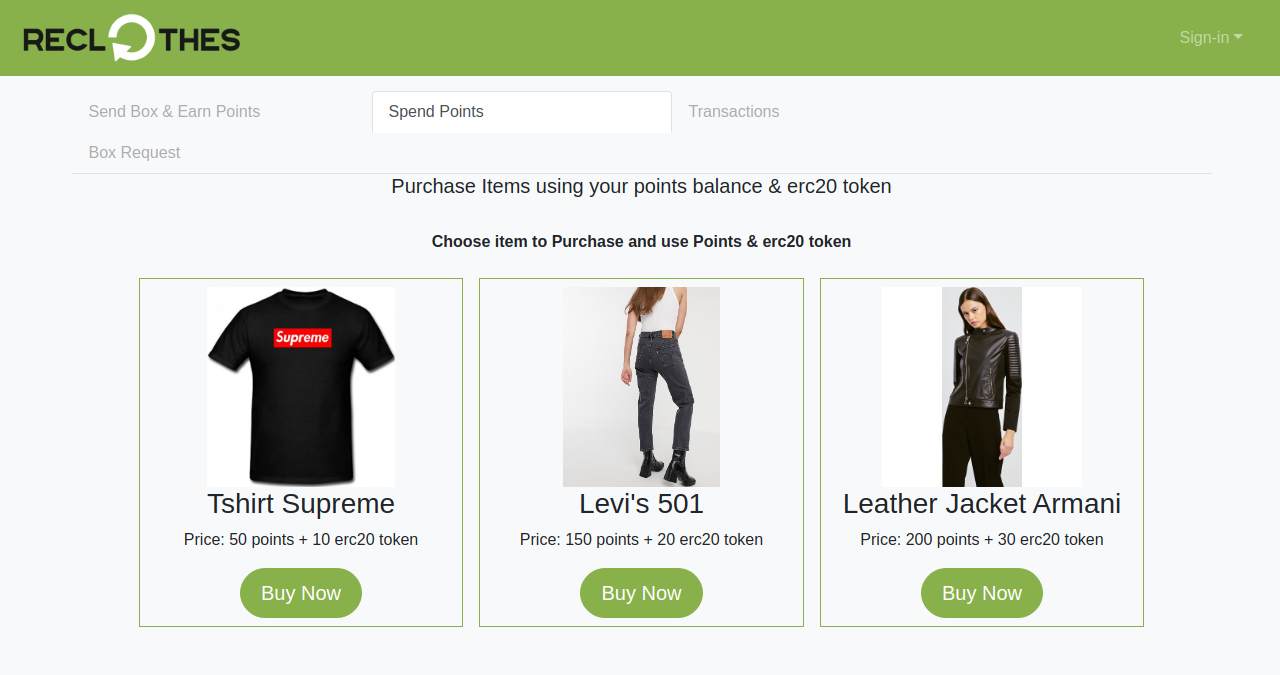
\includegraphics[totalheight=7.5cm]{img/dapp/user-buy.png}
    \caption{Purchase Clothes}
    \label{fig:purchase_clothes}
\end{figure}

\newpage
\subsubsection{Reclothes Admin Page}

In the previous sections, I explained the logical split about \textit{Admin for User} and \textit{Admin for Producers}.
In the following views, I divide the features related to the user type handled and there is a strong distinction about 
Users and Producers.

\paragraph{Admin For Users}

This section shows the views of the Admins that handle User side. Figure \ref{fig:evaluate_box} shows the field 
to compile in order to perform the evaluation, meanwhile, Figure \ref{fig:admin-tx} shows the transactions records.
Here a \href{https://ropsten.etherscan.io/tx/0x6688afff4f6adb7e334b87a2f078608ba11b0e0d884f54b52eac1cdde100a12e}{link} to a ropsten transaction.

\begin{figure}[h!]
    \centering
    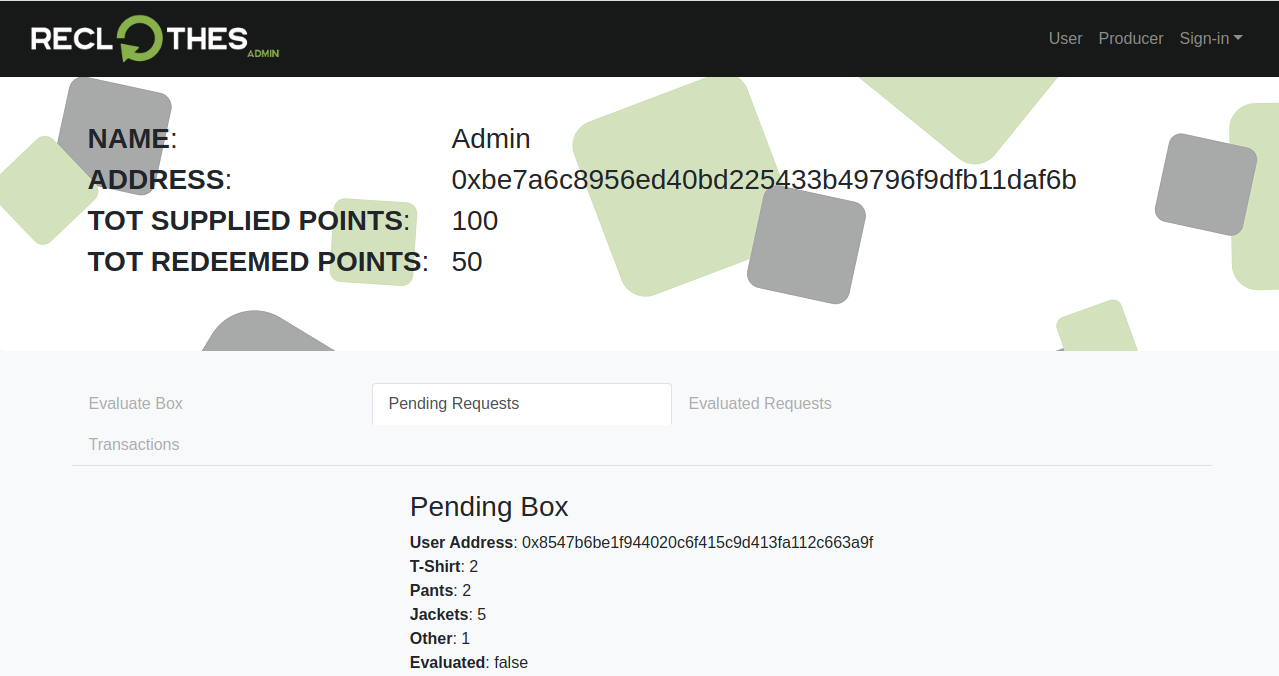
\includegraphics[totalheight=7.5cm]{img/dapp/admin-info.png}
    \caption{Admin Info}
    \label{fig:admin_info}
\end{figure}

\begin{figure}[h!]
    \centering
    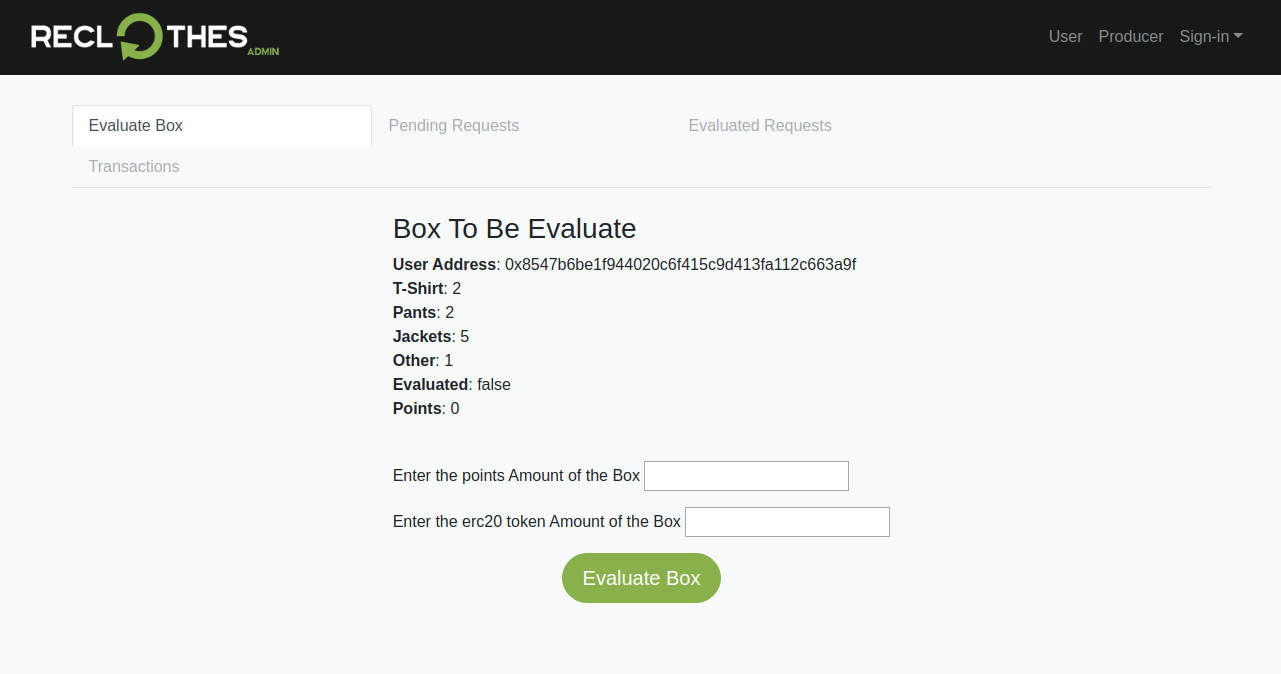
\includegraphics[totalheight=7.5cm]{img/dapp/admin-evaluate.png}
    \caption{Evaluate Box}
    \label{fig:evaluate_box}
\end{figure}

\begin{figure}[h!]
    \centering
    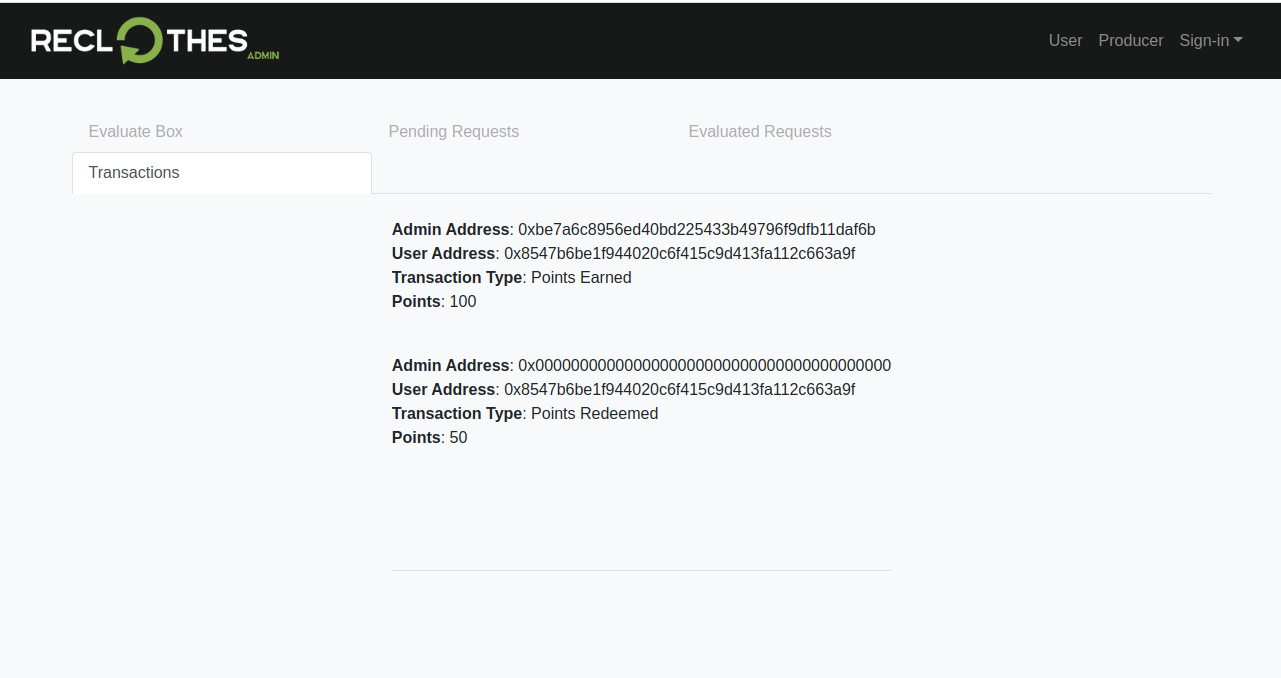
\includegraphics[totalheight=7.5cm]{img/dapp/admin-tx.png}
    \caption{Transactions}
    \label{fig:admin-tx}
\end{figure}

\paragraph{Admin For Producers}

This section shows the views of the Admins that handle Producer side. The Figure \ref{fig:adminp-info} 
shows all the Admin for Producers information's data. 

\begin{figure}[h!]
    \centering
    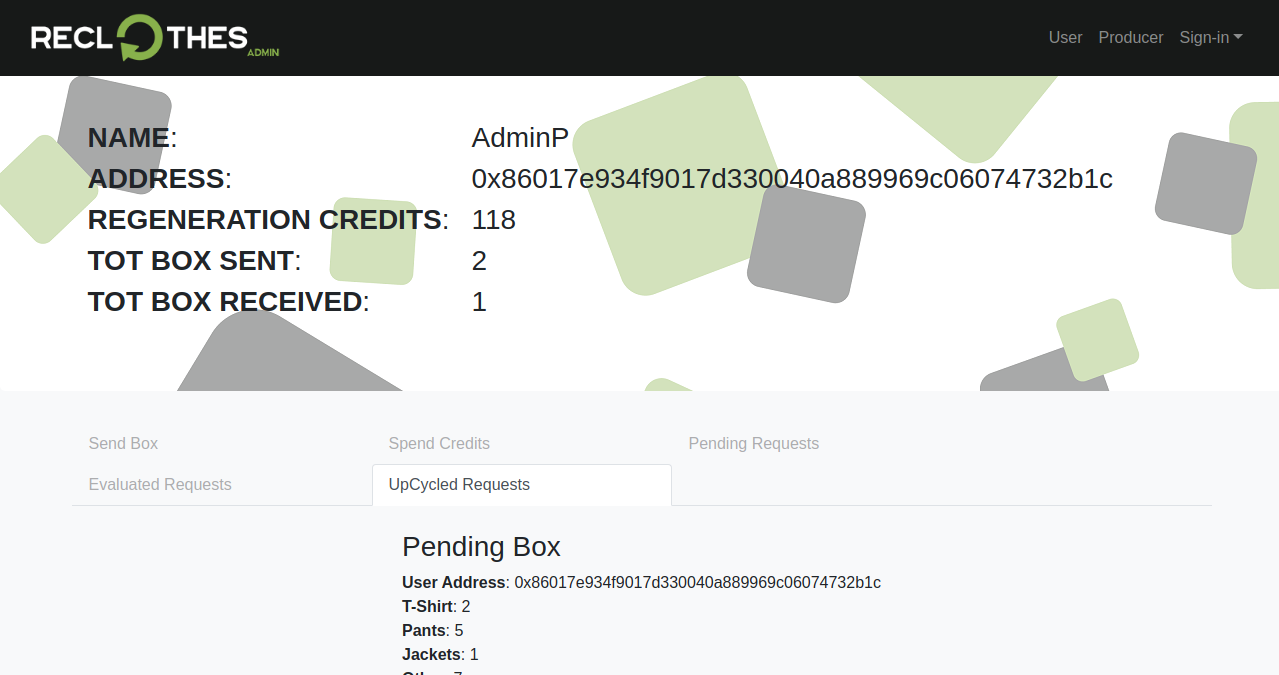
\includegraphics[totalheight=7.5cm]{img/dapp/adminp-info.png}
    \caption{Admin for Producers Info}
    \label{fig:adminp-info}
\end{figure}

\begin{figure}[h!]
    \centering
    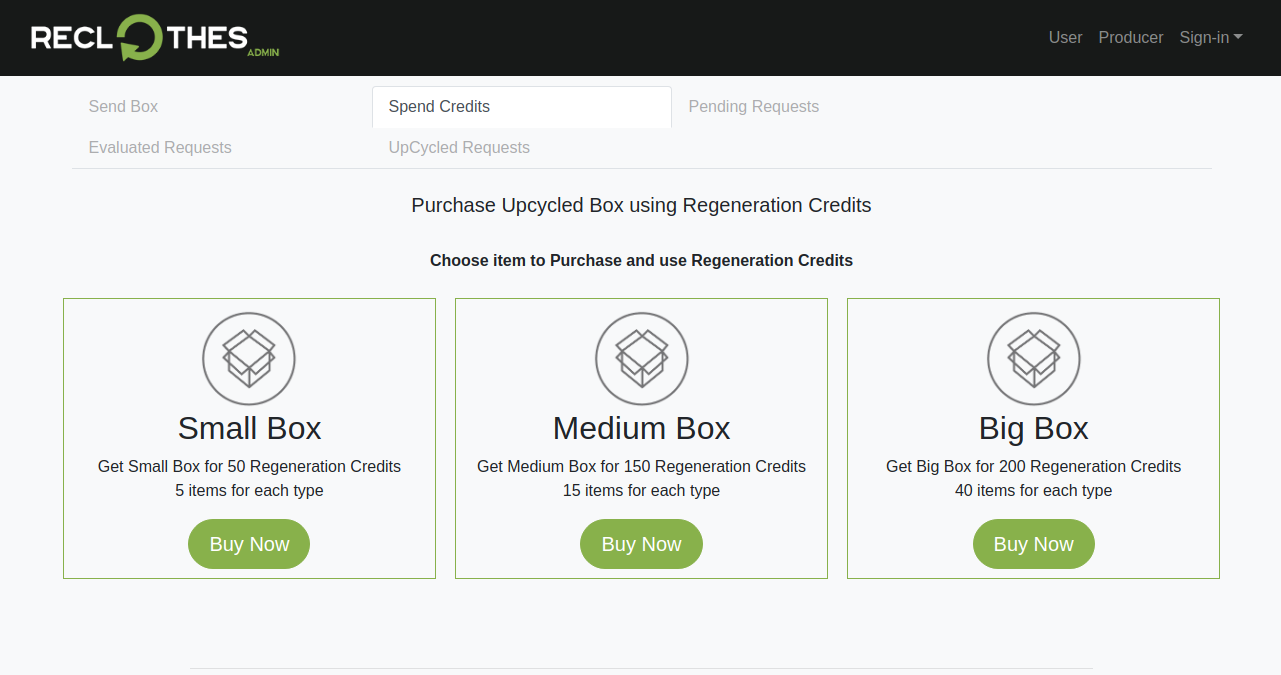
\includegraphics[totalheight=7.5cm]{img/dapp/adminp-buy.png}
    \caption{Admin Spend Regeneration Credits}
    \label{fig:adminp-buy}
\end{figure}

\newpage
\subsubsection{Producer}

This section shows the views of the Producer side. The evaluation process of the old materials
received by Reclothes is the same of the previous one.

\begin{figure}[h!]
    \centering
    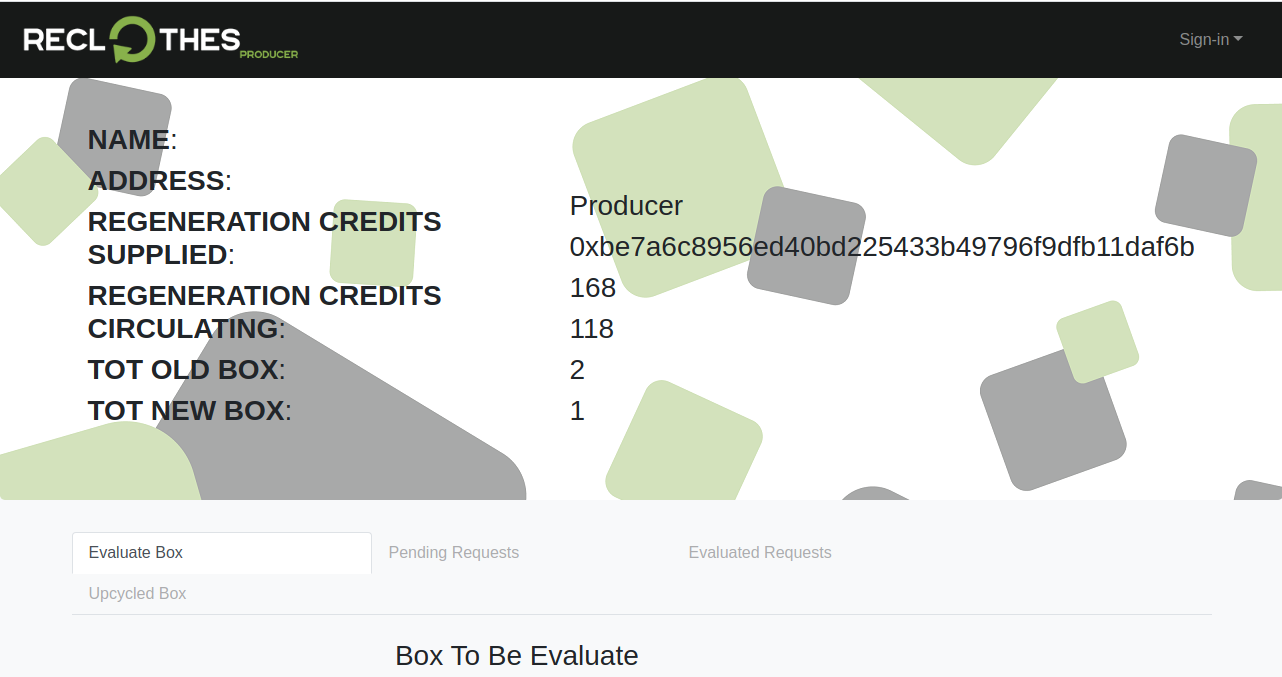
\includegraphics[totalheight=7.5cm]{img/dapp/producer-info.png}
    \caption{Producers Info}
    \label{fig:producer-info}
\end{figure}


\section{Cost Analysis}

\subsection{Hyperledger Fabric}

Hyperledger Fabric is a permissioned network and it doesn't have transaction fees. On the other hand the
companies that run own project over Fabric have to maintain the costs related to the node of the networks
created. There's several services and companies that sell hosting services related to Hyperledger network
nodes. 
\bigskip

To estimate the costs, our analysis is based on Amazon Managed Blockchain\cite{aws} test network owned by a single 
customer. This network has three Starter Edition members(1 each actors/organization) to simulate a multi-party transaction. 
Each member has a single \textbf{bc.t3.small} peer node with 20 GiB of storage and writes 9 MB to the network 
per hour.

\begin{outline}
    \1 \textbf{The hourly cost for this network is}:

    \2 \textbf{Membership cost}: (3 Starter Edition members) x (\$0.30 per hour) x (1 hour) = \$0.90 per hour
    \2 \textbf{Peer node cost}: (3 members) x (1 bc.t3.small peer node per member) x (0.034 per hour) x (1 hour) = \$0.102 per hour
    \2 \textbf{Peer node storage cost}: (3 members) x (1 peer node per member) x (20 GiB storage per peer node) x (\$0.10 per GB-month) x (1 hour) = \$0.009 per hour
    \2 \textbf{Data written cost}: (3 members) x (9 MB per hour) x (0.10 per GB) = \$0.003 per hour

    \1 \textbf{Total test network hourly cost}: \$1.014
    \1 \textbf{Total test network year cost}: \$8882.64
\end{outline}


\subsection{Ethereum}

The Ethereum Network prices is related to the transactions fees costs that depends on the data size 
of the transaction and on the gas price expressed in ether. The price for each gas defines
the transaction time, it means that more gas price corresponds to a less time of transaction computed 
and vice-versa. There are several features that going to influence the transaction fees over Ethereum 
network, such as ether price, or network traffic. 

The following price analysis is related to the current value of the ether that is \$237.36.\cite{gastracker} \cite{ethgasstation}

\begin{table}[h]
    {\renewcommand\arraystretch{1.25}
    \begin{tabular}{|l|l|l|} \hline
    \textbf{Gas Price} & \textbf{Confirmation Time} & \textbf{Transfer Price}\\ \hline\hline
    1 gwei & 128 secs \~ 2 minutes & \$0.005 \\ \hline
    34 gwei & 85 secs \~ 1 minutes 25 secs & \$0.17\\ \hline
    66 gwei & 13 secs & \$0.33\\ \hline
    \end{tabular}}
    \caption{Comparing among Ethereum transactions price}
    \label{table-compare-eth-price}
\end{table}

Considering 100.000 active Users. Each User on average sends 2 boxes with old clothes per year.
Therefore, Reclothes Side, the application performs 200.000 evaluation processes that belong to \textbf{200k} 
of incoming transactions per year. The incoming transaction number, multiplied for the minimum transaction cost, 
belongs to an overall cost of 200.000x\$0,005, which is \textbf{\$1000}.

Since there are just 70\% of active users, and considering an average of 10 purchasing per User every year. The 
Ethereum network has to process 70.000x10 = 700.000 transactions. Therefore as the above hypothesis to get the 
less cost per transaction; the overall costs of the outcome transaction is of 700.000x0,005 = \$3500.

In the end, the Ethereum network's overall cost is \$4500 per year. 

